\documentclass{report}

\usepackage{amsmath, amsthm, amssymb, amsfonts}
\usepackage{thmtools}
\usepackage{graphicx}
\usepackage{subcaption}
\usepackage{setspace}
\usepackage{geometry}
\usepackage{float}
\usepackage{hyperref}
\usepackage[utf8]{inputenc}
\usepackage[english]{babel}
\usepackage{framed}
\usepackage[dvipsnames]{xcolor}
\usepackage{tcolorbox}
\usepackage{multicol}
\usepackage{wrapfig}
\usepackage{minted}
\usepackage{tikz}
\usepackage{enumitem}

\usetikzlibrary{positioning, shapes.multipart, arrows.meta}

\colorlet{LightGray}{White!90!Periwinkle}
\colorlet{LightOrange}{Orange!15}
\colorlet{LightGreen}{Green!15}

\newcommand{\HRule}[1]{\rule{\linewidth}{#1}}

\declaretheoremstyle[name=Theorem,]{thmsty}
\declaretheorem[style=thmsty,numberwithin=section]{theorem}
\tcolorboxenvironment{theorem}{colback=LightGray}

\declaretheoremstyle[name=Proposition,]{prosty}
\declaretheorem[style=prosty,numberlike=theorem]{proposition}
\tcolorboxenvironment{proposition}{colback=LightOrange}

\declaretheoremstyle[name=Principle,]{prcpsty}
\declaretheorem[style=prcpsty,numberlike=theorem]{principle}
\tcolorboxenvironment{principle}{colback=LightGreen}

\setstretch{1.2}
\geometry{
    textheight=9in,
    textwidth=5.5in,
    top=1in,
    headheight=12pt,
    headsep=25pt,
    footskip=30pt
}

% ------------------------------------------------------------------------------
\tcbset{
    sharp corners,
    colback = white,
    before skip = 0.2cm,    % add extra space before the box
    after skip = 0.5cm      % add extra space after the box
}                           % setting global options for tcolorbox

\definecolor{main}{HTML}{5989cf}    % setting main color to be used
\definecolor{sub}{HTML}{cde4ff}     % setting sub color to be used

\newtcolorbox{boxH}{
    colback = sub, 
    colframe = main, 
    boxrule = 0pt, 
    leftrule = 6pt % left rule weight
}

\newcommand{\SubItem}[1]{
    {\setlength\itemindent{15pt} \item[-] #1}
}

\newcommand{\correct}{\item[\checkmark]}
\newcommand{\incorrect}{\item[$\times$]}

% ------------------------------------------------------------------------------

\begin{document}

% ------------------------------------------------------------------------------
% Cover Page and ToC
% ------------------------------------------------------------------------------

\title{ \normalsize \textsc{}
		\\ [2.0cm]
		\HRule{1.5pt} \\
    \LARGE \textbf{\uppercase{Advanced Information System Security}}
		\HRule{2.0pt} \\ [0.6cm] \LARGE{Hoping to get a better grade this time around.} \vspace*{10\baselineskip}}
\author{\textbf{Fabio Lorenzato}} 
		

\maketitle
\newpage

\tableofcontents
\newpage
\part{Theory}
\chapter{Transport Layer Security}
TLS, or Transport Layer Security, was originally proposed by Netscape
in 1995 as a way to secure communications between a web browser and a
web server. It is the successor to SSL, or Secure Sockets Layer, which
was first introduced by Netscape in 1995. The two terms are often used
interchangeably, but TLS is the more modern and secure protocol.\\ 
The main goal of SSL was to create secure network channel, almost at
session level(4.5), between two parties, to provide some security
services that neither TCP nor IP provides:
\begin{itemize}
  \item \textbf{peer authentication} based on asymmetric
    challenge-response authentication(the challenge for the service is
    implicit, while for the client is explicit). Server authentication
    is alway compulsory, while client authentication is optional and
    requested by the server.
  \item \textbf{message confidentiality} base on symmetric encryption
  \item \textbf{message integrity} and authentication based on MAC
    computed on the trasmitted data
  \item \textbf{replay, filtering and reordering attack protection}
    using implicit record numbers( the correct order of transmission
    is provided by TCP, for this reason the number is implicit). This
    number is used also in the MAC computation.

\end{itemize}

You can see the TLS packet structure in figure
\ref{fig:tls-packet-structure}.
The TLS handshake protocol is used to establish a new session or 
reestablish an existing session. The TLS change cipher spec protocol 
is used to trigger the change of the algorithms to be used for message 
protection, or most notably to pass from the previous unprotected 
session to a protected one. The TLS alert protocol is used to signal
errors or signal the end of the connection. 
The TLS record protocol contains the generic protocols informations
and its content depend of the state of the connection and the protocol
it is tunneling.
\begin{figure}[H]
    \centering
    \includegraphics[width=.6\textwidth]{img/TLS packet
    structure.png}
    \caption{TLS packet structure.}
    \label{fig:tls-packet-structure}
\end{figure}

\section{TLS session and connection}
It is important to make a clear distinction between TLS session and
connections.\\
\textbf{TLS sessions} a \textbf{logical association} between client and server, created
via an handshake protocol and its shared between different TLS
connections(1:N).\\
\textbf{TLS connections} are a \textbf{transient TLS channel} between client and server,
which means that each connection is associated with only one specific
TLS session(1:1).

\begin{figure}[H]
  \centering
  
\includegraphics[width=.7\textwidth]{img/TLS session connection.png}
  \caption{TLS session and connection.}
  \label{fig:tls-session-and-connection}
\end{figure}
\section{TLS handshake protocol}
The TLS handshake protocol is used to establish a new session or
reestablish an existing session. It's a critical part of the TLS
protocol, because the channel pass from an unprotected state to a
protected one. During this phase the two parts agree
agree on a set of algorithms for confidentiality and integrity,
exchange random numbers between the client and the server to be used
for the subsequent generation of the keys, establish a symmetric key
by means of public key operations (originally RSA and DHKE, but
nowadays the elliptic curve versions of algorithms are used) and negotiate the
session-id and exchange the necessary public keys certificates for the
asymmetric challenge-response authentication.

\section{Achieving Data protection}
Data protection is achieved by using symmetric encryption algorithms
to encrypt the data and Message Authentication Codes(MAC) to ensure
the integrity of the data and the authentication of the sender.\\
Figure \ref{fig:tls-data-protection} shows how the data protection is 
achived in TLS using authenticate-then-encrypt approachm, but also
encrypt-then-authenticate is possible.\\
The MAC is computed over the data(compressed or not), the TLS sequence 
number and the key used for the MAC computation. The padding is also
part of the MAC computation to avoid those attacks that change the
padding.\\
The MAC is then encrypted with the dedicated symmetric key and a
suitable initialization vector(IV) 

\begin{figure}[H]
  \centering
  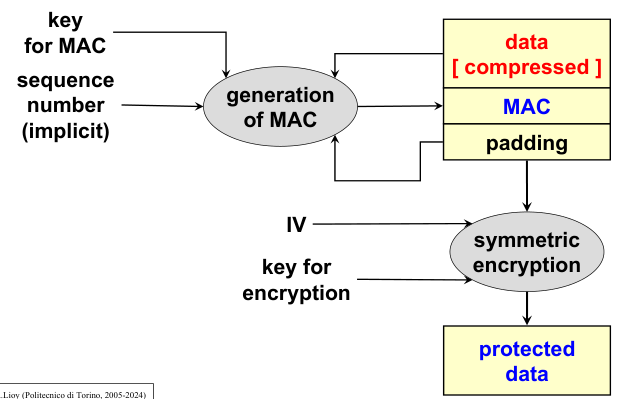
\includegraphics[width=.5\textwidth]{img/TLS data protection.png}
  \caption{TLS data protection.}
  \label{fig:tls-data-protection}
\end{figure}

The keys are \textbf{directional}, so there are two keys( one for
client to server and one for server to client) to protect against
reuse of the sequence number in the opposite direction.

\section{Relationship among keys and sessions}
When a new session is created using the handshake protocol, a new
\textbf{pre-master secret} is established using public key
cryptography. Then from the session a new connection is created, which
requires a random number to be generated, and exchanged between the
client and the server. Those two values are combined via a KDF,
usually HHKDF( HMAC-based key derivation function) to generate the 
\textbf{master secret}. This computation is done only once, and the 
secret is common to several connections.\\
The pre-master secret is then discarded, and the keys necessary for
the MAC computation, encryption and, if necessary, IVs will be derived
from the master secret.\\
You can notice that the master secret is common to any connections
inside a session, but the per-connection keys are different every
time. This is another important feature to avoid replay attacks,
possible because numbering is per-connection. This solution also
allows to reduce the cost of establishing new keys for each
connection.

\begin{figure}[H]
  \centering
  \includegraphics[width=.5\textwidth]{img/relationship
  keys-connection.png}
  \caption{Relationship among keys and sessions.}
  \label{fig:tls-keys-and-sessions}
\end{figure}

\section{Perfect Forward Secrecy}
Since the keys are generated from symmetric crypto, if the private key
used to perform encryption and decryption of the pre-master secret is
compromised, all the previous communication can be decrypted because
it is possible to derive the master-secret. This is only possible if
the server has a certificate valid for both signature and encryption
In this context, perfect forward secrecy is desirable.
\begin{boxH}
  \textbf{Perfect Forward Secrecy} is a property of key-agreement
  protocols ensuring that the compromise of the secret key used for 
  will compromise only current (and eventually future) traffic but not
  the past one
\end{boxH}
The most common way to achieve this is to use \textbf{ephemeral keys},
which are one-time asymmetric keys( used for key exchange). This means
that the key pair used for key exchange is not a long term key pair,
but a temporary one generated on-the-fly when necessary.\\ 
The ephemeral key needs to be authenticated, so only for this purpose
the long-term key is used for signing the ephemeral key. This is done
using DHKE instead of RSA because the latter one is really slow, while
the former one is faster with the compromise of only using the
established key for a certain number of session.\\
Let's now go over some considerations: if the temporary key is
compromised, perfect forward secrecy of the communication is still
valid because he can only decrypt the traffic exchanged using the
temporary key. On the contrary, if the long-term key is compromised,
no secret is really disclosed, because no traffic has been exchanged
using it for encryption, but is still a problem for server
authentication.

\section{The protocol}
The TLS handshake is always initiated by the client. 

\subsection{Client Hello and Server Hello}
In version 1.2 the client sends a \textbf{Client Hello}, which
contains:
\begin{itemize}
  \item the SSL version preferred by the client, and the highest
    supported(2=SSL-2, 3.0=SSL-3, 3.1=TLS-1.0, \dots)
  \item a 28 bytes pseudo-random number, which is the client random
  \item a session-id, which is \textit{0} if the client is starting a
    new session, and \textit{1} if the client is trying to resume a
    previous session
  \item a list of cipher suites supported by the client, in order to 
    let the server choose the most secure one (the set of algorithms
    used for encryption, for key exchange, and for integrity)
  \item a list of compression methods supported by the client
    (supported only up to TLS 1.2)
\end{itemize}

And then a \textbf{server hello} is sent back, which contains:
\begin{itemize}
  \item the SSL version chosen by the server, the highest one
    supported by both the client and the server
  \item a 28 bytes pseudo-random number, which is the server random
  \item a session identifier(session-id), which is a new one if the
    server is starting a new session, and the same as the client's if
    the server is resuming a previous session
  \item the cipher suite chosen by the server, the strongest common
    one between the client and the server
  \item the compression method chosen by the server
\end{itemize}


\begin{figure}[H]
  \centering
  \begin{subfigure}{.5\textwidth}
    \centering
    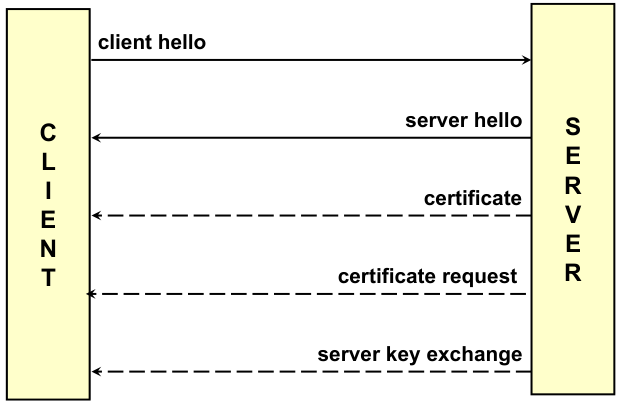
\includegraphics[width=.9\linewidth]{img/TLS key echange.png}
    \caption{The TLS handshake protocol(TLS 1.2).}
    \label{fig:tls-handshake-protocol-1.2}
  \end{subfigure}%
  \begin{subfigure}{.5\textwidth}
    \centering
    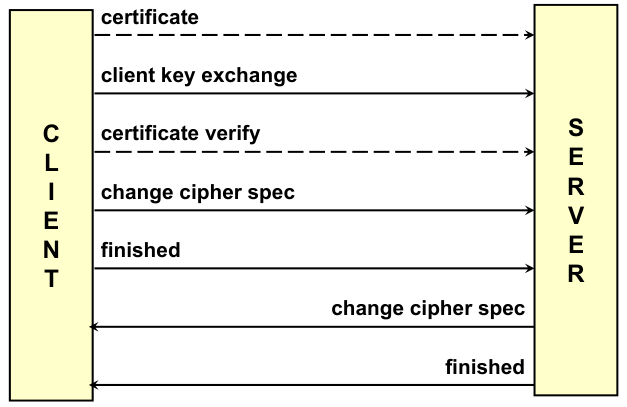
\includegraphics[width=.9\linewidth]{img/TLS key exchange 1-3.png}
    \caption{The TLS handshake protocol(TLS 1.3).}
    \label{fig:tls-handshake-protocol-1.3}
  \end{subfigure}
\end{figure}

\subsection{Cipher suite}
A cipher suite is a string which contains the set of cryptographic
algorithms used in the TLS protocol. A typical cipher suite consists
of a key exchange algorithm, the symmetric encryption algorithm, and
the hash function used for generating MACs.
Some example of those are:
\begin{itemize}
  \item SSL\_NULL\_WITH\_NULL\_NULL (no protection, used for the record
    protocol to be used in the handshake)
  \item SSL\_RSA\_WITH\_NULL\_SHA
  \item SSL\_RSA\_EXPORT\_WITH\_RC2\_CBC\_40\_MD5
  \item SSL\_RSA\_WITH\_3DES\_EDE\_CBC\_SHA
\end{itemize}


\subsection{Certificates}
After the initial exchange, the server is ready to authenticate
itself.\\
The server sends its long-term public key certificate to the client
for server authentication. Actually, the whole certificate chain, up
to the root CA, must be sent. Furthermore , the subject of the 
certificate must match the server name.\\
Server authentication is implicit, because its private key is used to
decrypt the pre-master secret, while client authentication is 
always explicit.

\begin{boxH}
  The implicit server authentication is based on the fact that the MAC
  is computed trough the key derived trough knowledge of the private
  key, so only the server can compute it.
\end{boxH}

Optionally, the server can request a certificate from the client for
client authentication. In this case the server specifies the list of
trusted CA's, and the client sends its certificate chain. The browsers
show to the users (for a connection) only the certificates issued by
trusted CAs.
If client certificate verification is required, an explicit request to
send the hash computed over all the handshake messages before this 
one and encrypted with the client private key is sent to the client.

\subsection{Key exchange}
The key exchange is the most important part of the handshake protocol.
If the server is using RSA for key exchange, the client generates a
pre-master secret, encrypts it with the server's public key(which can
be ephemeral or from its x.509 certificate) and sends it to the
server. If RSA is no used, DHKE can be used to generate the pre-master
secret, and in this case the server computes the value independently 
and the two parts can derive the master secret.\\
Another option is to use FORTEZZA, which is a key exchange algorithm
based on DH.

\subsection{Certificate verify}
In case the server requested client authentication, the client will be
required to send the certificate to prove that he is the owner of it's
private key. The message to be signed is the hash of all the messages
exchanged up to this point in the handshake protocol. This is to avoid
replay attacks too.


\subsection{Change cipher spec}
The change cipher spec message used to trigger the change of the
algorithms to be used for message protection. It allows to pass from
the previous unprotected messages to the protection of the next
messages with algorithms and keys just negotiated, thus is technically
a protocol on its own and not part of the handshake. Some analysis
even say that it could be removed from it.


\subsection{Finished message}
The finished message is the last message of the handshake protocol,
and the first message protected by the negotiated keys and algorithms.
It is necessary to ensure that the handshake has not been tampered
with, and it contains contains a MAC computed over all the previous
handshake messages (but change cipher spec) using as a key the master
secret. Notice that the finished message is different for the client 
and the server, because the MAC is computed over different messages.

This allows to prevent rollback man-in-the-middle attacks (version
downgrade or ciphersuite downgrade)

% 3 subfig, 2 on top and 1 on bottom
\begin{figure}[H]
  \centering
  \begin{subfigure}{.5\textwidth}
    \centering
    \includegraphics[width=.9\linewidth]{img/TLS no ephimeral no
    auth.png}
    \caption{TLS handshake(no ephemeral, no client authN).}
    \label{fig:tls-handshake-protocol}
  \end{subfigure}%
  \begin{subfigure}{.5\textwidth}
    \centering
    \includegraphics[width=.9\linewidth]{img/TLS no ephimeral
    auth.png}
    \caption{TLS handshake(no ephemeral, client authN).}
    \label{fig:tls-handshake-protocol-2}
  \end{subfigure}
  \begin{subfigure}{.5\textwidth}
    \centering
    \includegraphics[width=.9\linewidth]{img/TLS ephimeral no
    auth.png}
    \caption{TLS handshake(ephemeral, no client authN).}
    \label{fig:tls-handshake-protocol-3}
  \end{subfigure}
  \caption{TLS handshake protocol.}
\end{figure}

\section{Setup Time}
The setup time is the time required to establish a secure connection 
between the client and the server. TLS depends on TCP, so the TCP
handshake must be taken into account. Then the TLS handshake is
performed, meaning that typically 3 RTTs (1 for TCP and 2 for TLS) are
required to establish a secure connection. Usually after 180ms the two
parties are ready to send protected data( assuming 30ms delay
one-way).

% 2 subfig
\begin{figure}[H]
  \centering
  \begin{subfigure}{.5\textwidth}
    \centering
    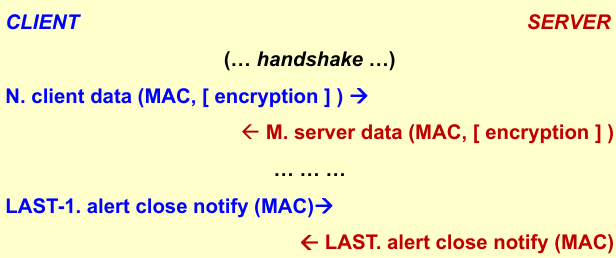
\includegraphics[width=.9\linewidth]{img/TLS link teardown.png}
    \caption{TLS link teardown.}  
    \label{fig:tls-link-teardown}
  \end{subfigure}%
  \begin{subfigure}{.5\textwidth}
    \centering
    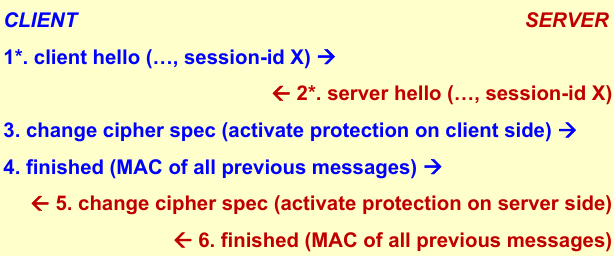
\includegraphics[width=.9\linewidth]{img/TLS resume session.png}
    \caption{TLS resume session.}
    \label{fig:tls-resume-session}
  \end{subfigure}
  \caption{TLS link teardown and resume session.}
\end{figure}

\section{TLS versions}
\subsection{TLS 1.0}
TLS 1.0, or SSL 3.1, was released in 1999. It is the first version of
the protocol, and it is based on SSL 3.0. Previous version were using
proprietary solutions, so the adoption of open standards was strongly
encouraged.

\subsection{TLS 1.1}
TLS 1.1 was released in 2006, and it introduced some security fixes
especially to protect against CBC attacks. In fact, the implicit
IV is replaced with an explicit IV to protect against CBC attacks.
Also protection against padding oracle attacks were introduces to
reduce the information leaks. For this reason Passing errors now use
the bad\_record\_mac alert message (rather than the decryption\_failed
one). Furthermore, premature closes no longer cause a session to be non-
resumable.

\subsection{TLS 1.2}
TLS 1.2 was released in 2008, and it introduced some new features and 
improvements. The chipersuite also specifies the pseudo random
function instead of leaving the choice to the implementation. The
sha-1 algorithm was replaced with SHA-256, and its also added support
for authenticated encryption, such as AES in GCN or CCM mode.

All the chipersuites tat use IDEA and DES are deprecated.

\section{TLS attacks}
\subsection{Heartbleed}
Heartbleed is a security bug in the OpenSSL cryptography library,
which is a widely used implementation of the TLS protocol. It was able
to exploit the fact that the heartbeat extension keeps the connection
alive without the need to negotiate the SSL session again. The
attacker could send a heartbeat request, but the length of the 
response is much longer( up to 64KB) than the actual data sent by the
client. This attack could then allow to leak memory contents.

\subsection{Bleichenbacher attack}
Blackenbacker is a 1998 attack and it's the so-called the million
message attack because it exploited a vulnerability in the way the RSA
encryption was done. RSA requires the padding to be done in a certain
way, because if it is unoptimally done, it could cause some issues.\\
The attacker could perform an RSA private key operation with a
server’s private key by sending a million or so well-crafted messages
and looking for differences in the error codes returned. By basically
knowing the public key and trying to decrypt a message with some
guessed private keys, the different responses obtained were giving
hints about which bits were correct and which bits were wrong.\\
Later one the RSA implementations moved to RSA-OAEP, which is a
padding scheme that is provably secure against chosen-ciphertext
attacks.\\
In 2017 another variant of this attack was discovered, called
ROBOT( Return Of Bleichenbacher's Oracle Threat), to which many major
websites, like Facebook, were vulnerable.

\subsection{Other attacks against SSL/TLS}
Some other attacks against SSL/TLS are CRIME, BREACH, BEAST and
POODLE.\\
\textbf{Crime} is an attack against the \textbf{compression algorithm}
used in \textbf{SSL/TLS}, which by injection chosen plaintext in the
user requests, for example by using a form or choosing fraudulently an
username that is displayed, and then measure the size of the encrypted
traffic, an attacker could recover specific plaintext parts exploiting
information leaked from the compression, and this is part of the
reason why the compression is deprecated in TLS 1.3.\\
\textbf{BREACH} is an attack against the \textbf{HTTP compression} to
deduce a secret within the HTTP response provided by the server. It is
different from Crime because the former is an attack against the
compression algorithm used in SSL/TLS, while the latter is an attack
against the HTTP compression.\\
\textbf{BEAST} is an attack that exploits a vulnerability in the way
the \textbf{CBC} mode of operation is used in SSL/TLS. The attack is
possible if \textbf{IV concatenation}is used, meaning that the initial
vector for the next encryption is taken from the end of the previous
encryption. A MITM may decrypt HTTP headers with a blockwise-adaptive
chosen-plaintext attack, and by doing so, he's able to decrypt HTTPS
requests and steal information such as session cookies.\\
\textbf{POODLE}, or Padding Oracle On Downgraded Legacy Encryption, is
an attack that exploits the fact that SSL 3.0 uses a padding scheme
that is vulnerable to a \textbf{padding oracle attack}, by acting as a
MITM. This is done by exploiting SSL-3 fallbacks to decrypt data. This
is also the only attack among those that still works today.\\
\textbf{FREAK}, or Factoring RSA Export Keys, is an attack that
exploits the downgrades on TLS to export-level RSA keys to a
factorizable bit length(512 bits). It is also possible to carry this
out by downgrading the symmetric key too and then perform a brute
force attack( 40-bit). As you can see from figure
\ref{fig:freak-attack}, in the first phase the random and the
supported elliptic curve are not altered by the MITM, but only the
supported cipher suites are altered( to export level ones). Usually 40
bits chiper suits should not be configured at all, but some
misconfigurations may happen. The third phase is where the magic
happen: we have theoretically the MAC  in the FINISHED message to
protect against tampering (recall that the MAC will be computed over
all the handshake messages) but since the MAC is protected with the
master secret, the master secret is only 40 bits. The attacker can
then brute force the master secret on-the-fly, recompute the MAC so
that the server will accept the message. Since the attacker have
access to the premaster secret and the master secret, all traffic
beyond this point is encrypted with a weak shared key and the
middleman can read and even modify the traffic.\\
For all those reasons SSL-3 has been disabled on most browsers, but
its still needed for some browsers, for example IE6 by Microsoft,
which is outlasting its expected life span, because its the default
browser on Windows XP, which is still used today unfortunately,
meaning that the window of exposure for those attacks is still open.

\begin{figure}[H]
  \centering
  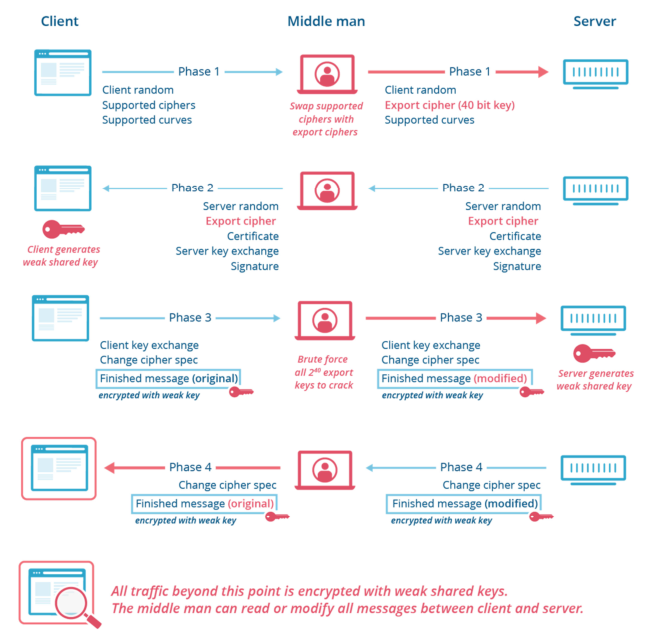
\includegraphics[width=.6\textwidth]{img/FREAK attack.png}
  \caption{FREAK attack.}
  \label{fig:freak-attack}
\end{figure}

\section{ALPN extension}
The ALPN extension, or Application-Layer Protocol Negotiation, is an
extension that allow to negotiate the application protocol to speed up
the connection creation, avoiding additional round-trips for
application negotiation. It is used to negotiate the protocol to be 
used on top of the TLS connection, such as HTTP/2, SPDY, or QUIC,
before the connection is established. This is useful because it saves
time, obviously, because after the connection is established, the
client and server could still fail to communicate because the
application protocol is not supported by the server.\\
The extension is inserted in the client hello message, by setting the
ALPN flag to true and providing a list of supported protocols in the
client HELLO message. The server will respond with the ALPN flag set
to true(if it supports the extension) and the selected protocol.\\
This is also useful for those servers that use different certificates
for the different application protocols.

\section{TLS False Start}
TLS False Start is another extension that allows the client can send
application data together with the ChangeCipherSpec and Finished
messages, in a single segment, without waiting for the corresponding
server messages. The biggest advantage of using this is the reduction
of the latency to 1 RTT. In theory this should work without changes,
but to use this in Chrome and Firefox they require the ALPN and the 
Forward Secrecy enabled, while Safari requires forward secrecy.

\section{The TLS downgrade problem}
In theory, when negotiating the TLS version to be used, the client
sends (in ClientHello) the highest supported version, while the server
notifies (in ServerHello) the version to be used (highest in common
with client).\\
For example if the client support up to SSL 3.3(TLS 1.2) and the
server support the same version, the connection will be established
using TLS 1.2. But if the server supports only SSL 3.2(TLS 1.1), the
connection will be established using SSL TLS 1.1.\\
Some servers, instead of sending the highest version supported, just
close the connection, forcing the client to retry with a lower version
of the protocol. An attacker could exploit this behavior to force the
client to use an older version of the protocol, by repeatedly closing
the connection, and then exploit the vulnerabilities of the older
version of the protocol.\\
\begin{boxH}
  This means that its not a problem of the protocol itself, but of the
  implementation of the server.
\end{boxH}

\subsection{TLS Fallback Signalling Cipher Suite Value (SCSV)}
This behavior is not always an attack, for example there could be and
error in the channel, which is closed by the server. This means that
there's a need to distinguish between a real attack and a simple 
error.\\
The \textbf{TLS Fallback SCSV} is a \textbf{special value} that is
used to prevent the protocol downgrade attacks, not only chiper suite.
It do so by sending a new (dummy) ciphersuite
value(TLS\_FALLBACK\_SCSV) which is sent by the client when opening a
downgraded connection as the last value in the chipersuite list.\\
If the server receives this value and still supports an higher version
of the protocol, it will know that the client is trying to downgrade
the connection, and it will refuse to establish the connection by
sending a \textbf{inappropriate\_fallback} alert message an closing
the channel.\\
This notify the client that he should retry with the highest version 
of the protocol supported by himself.\\
Many servers do no support SCSV yet, but most servers have fixed their
behavior when the client requests a version higher than the supported
one so browsers can now disable insecure downgrade

\section{TLS session tickets}
We know that session resumption is possible with TLS, but the server
needs to keep a cache of session IDs, which may become very large for
high traffic servers. For this reason, the \textbf{TLS session
tickets} were introduced, which are an extension allowing the server
to send the session data to the client encrypted with a server secret
key. This data is stored by the client, which will send it again when
it wants to resume a session. This allows to move the cache to the
client side. Obviously, this data has to be encrypted with a server
secret key.\\
Even if this behaviour is desirable for the server, it still need to
be supported by the browser ( it's an extension after all) and needs a
mechanism to share keys among the servers in a load-balancing heavy
environment.
\section{The Virtual Server Problem}
Nowadays, virtual servers are very common in web hosting, because they
allows to have different logical names associated with the same IP
address( ie: home.myweb.it=10.1.2.3, food.myweb.it=10.1.2.3).
This is easy to manage in HTTP/1.1 but quite troublesome with HTTPS,
because TLS is activated before the HTTP request is sent, which makes
it difficult to know which certificate should be provided in advance.
The solutions are quire simple:
\begin{itemize}
  \item use a wildcard certificate, which is a certificate that is
    valid for all the subdomains of a domain (ie: *.myweb.it)
  \item use the SNI (Server Name Indication) extension, which is an
    extension that allows the client to specify the hostname of the
    server it is trying to connect to, allowing the server to provide
    the correct certificate. This is sent in the ClientHello message.
  \item provide a certificate with a list of servers in
    subjectAltName, which allow to share the same private key for 
    different servers.
\end{itemize}

\section{TLS 1.3}
TLS 1.3 was released in 2018, and it introduced some new features
while solving some of the most common problems of the previous 
versions:
\begin{itemize}
  \item \textbf{reduce} the \textbf{handshake latency} in general 
  \item \textbf{encrypting} more of the \textbf{handshake} (for
    security and privacy, after all up to TLS 1.2 the handshake was in
    clear text)
  \item \textbf{improving resiliency} to cross-protocol attacks
  \item removing legacy features
\end{itemize}
We will now go over the main changes in TLS 1.3.

\subsection{Key exchange}
In this version, the support for static RSA and DH key exchange was
removed for many reasons:
\begin{itemize}
  \item it does not implement forward secrecy 
  \item its difficult to implement correctly, which is a problem
    because it exposes the system to many attacks like Bleichenbacher
\end{itemize}
Now Diffie-Hellman ephemeral (DHE) and Elliptic Curve Diffie-Hellman
Ephemeral (ECDHE) are the only key exchange methods supported, with
some required parameters( some implementations weren't really up to
the standards, ie: used DH with small numbers( just 512 bits) or
generated values without the required mathematical properties).

\subsection{Message protection}
TLS 1.3 greatly improves message protection by eliminating several
vulnerabilities present in earlier versions. Previously, issues arose
from using CBC mode with authenticate-then-encrypt, which led to
attacks like Lucky13 and POODLE. The use of RC4 also allowed plaintext
recovery due to measurable biases, and compression enabled the CRIME
attack.\\
TLS 1.3 addresses these weaknesses by removing CBC mode and enforcing
AEAD modes for stronger security. Insecure algorithms such as RC4,
3DES, Camellia, MD5, and SHA-1 have been dropped, and compression is
no longer used, ensuring a more secure cryptographic environment.

\subsection{Digital signature}
In TLS 1.3, digital signatures have been strengthened to address
earlier vulnerabilities. Previously, RSA signatures were used on
ephemeral keys with the outdated PKCS\#1v1.5 schema, leading to
potential flaws. The handshake was authenticated using a MAC instead
of a proper digital signature, which exposed the protocol to attacks
like FREAK.\\
TLS 1.3 improves this by using the modern, secure RSA-PSS signature
scheme. Additionally, the entire handshake is signed, not just the
ephemeral keys, providing more comprehensive security. The protocol
also adopts modern signature schemes, enhancing the overall strength
of the cryptographic process.

\subsection{Ciphersuites}
TLS 1.3 simplifies the protocol by reducing the complexity seen in
earlier versions, which had a long list of cryptographic options that
grew exponentially with each new algorithm. This complexity made
configuration and security management difficult.\\
To address this, TLS 1.3 specifies only essential, orthogonal
elements: a cipher (and mode) combined with an HKDF hash function. It
no longer ties the protocol to specific certificate types (like RSA,
ECDSA, or EdDSA) or key exchange methods (such as DHE, ECDHE, or
PSK).\\
Moreover, TLS 1.3 narrows the selection to just five ciphersuites:
\begin{itemize}
  \item TLS\_AES\_128\_GCM\_SHA256
  \item TLS\_AES\_256\_GCM\_SHA384
  \item TLS\_CHACHA20\_POLY1305\_SHA256
  \item TLS\_AES\_128\_CCM\_SHA256
  \item TLS\_AES\_128\_CCM\_8\_SHA256 (deprecated but yet supported
    for computational environments with low capacity)
\end{itemize}

\subsection{EdDSA}
\textbf{EdDSA}, or Edwards-curve Digital Signature Algorithm, is a digital 
signature scheme using the EdDSA signature scheme, which is a variant
of the standard elliptic curve DSA schema. The EdDSA scheme,
unlike standard DSA, doesnt require a PRNG, which could in some cases
leak the private key if the underlying generation algorithm is broken
or predictable.\\
EdDSA picks a nonce based on a \textbf{hash of the private key} and
the \textbf{message}, which means after the private key is generated
there’s no need anymore for random number generators. Another
advantage is that the EdDSA is faster in signature generation and
verification than the standard DSA, because it implements simplified
point addition and doubling.\\
EdDSA is using an n-bit private and public keys and will generate a
signature which has a size which is the double of the keys size.
As per the RFC stipulations, EdDSA must support the Ed25519 and
Ed448 curves, which are based on the Edwards-curve Digital Signature,
which uses respectively SHA-2 and SHA-3 as hash functions. Among those
two, Ed25519 is the most used, which is also used for an
implementation of EcDH.\\
When it comes to the RFCs there's an issue: there are two RFCs that 
are slightly different, one is the RFC 8032, which is for general
internet implementations, with the implementational details left to
the developers, and there's also FIPS 186-5, which specifies not only
the mathematics behind an algorithm but also implementation details
because it is a standard for the US government.


\subsection{Other improvements}
TLS 1.3 introduces several key improvements to enhance security and
efficiency. One major change is that all handshake messages sent after
the ServerHello are now encrypted, ensuring better confidentiality
during the handshake process, even if the keys have not been
enstablished(we will go over the details later). The new
\textbf{EncryptedExtensions} message allows additional extensions,
which were previously sent in cleartext during ServerHello, to also
benefit from encryption, improving privacy.\\
Additionally, key derivation functions have been redesigned to support
easier cryptographic analysis due to their clear key separation
properties. HKDF is now used as the underlying primitive for key
derivation, providing a robust and flexible method.\\
The handshake state machine has also been overhauled, making it more
consistent by removing unnecessary messages, such as
\textbf{ChangeCipherSpec}, which is now only retained for
compatibility with older systems. This restructuring streamlines the
handshake process, reducing complexity and improving protocol
efficiency.


\subsection{HKDF in TLS 1.3}
HKDF is one of the novelties of TLS 1.3, and is a HMAC-based
extract-and-expand Key Derivation Function. As a normal key derivation
function, it takes 4 inputs: the salt, the input keying material(
which is basically a secret key), the info string and the output
length. It basically takes the first 2 inputs to derive a key which
will be used to derive a pseudorandom key .Then the second stage
expands this key into several additional pseudorandom keys, which are
the output of the KDF. So multiple outputs can be generated from the
single IKM value by using different values info strings.\\
By calling the function repeatedly call the HMAC function with with PR
keys and the info string as the input message, and then concatenate 
the results, by appending the output of the HMAC function to the 
previous output and incrementing an 8-bit counter.\\
This means that from one call we can generate at most 256($2^8$)
different keys.\\
The finished message is not protected with the master secret as it was
in TLS 1.2, but with the specific key, which is created with expand
starting from the base key and putting as info the text "finished" and
then the desired length. The pre-shared key to protect the ticket
contains the word "resumption". So you start with some basic key
material and then by using different labels, you are able to generate
the different keys.

\begin{listing}[H]
  \begin{minted}{python}
    HKDF-Expand( HKDF-Extract ( salt, IKM ), info, length )
  \end{minted}
  \caption{HKDF-Expand pseudocode.}
  \label{lst:hkdf-expand}
\end{listing}

\subsection{TLS-1.3 handshake}
Even the handshake in TLS 1.3 was changed. The first thing that we
notice is that the change chiper specs has been removed from the
standard.\\
At first, as you can see from figure \ref{fig:tls-1.3-handshake}, the
connection starts with an hello message from the client, which will
also send it's list of chipersuites and the key share material , in
which the client will send it's DH parameters(it is still needed after
all). All this data is sent in the same message to save some RTTs and
to allow the middleboxes with lower TLS version support to understand 
the message, interpreting them as an extension of the client hello and
thus skipping them. In fact most of the TLS 1.3 features are 
implemented in message extensions.\\
The following messages are just the specular ones but sent from the
server this time. After this point it is possible to have
confidentiality of the communication, because a shared key has been
established(the curly braces in the picture are just for that).\\

\begin{figure}[H]
  \centering
  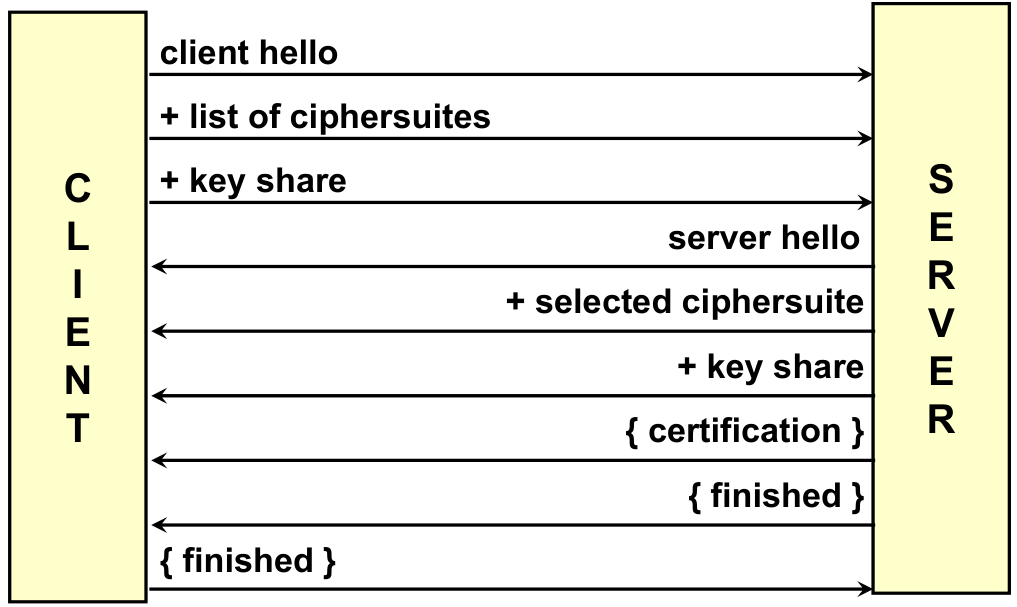
\includegraphics[width=.6\textwidth]{img/TLS 1-3 handshake.png}
  \caption{TLS 1.3 handshake.}
  \label{fig:tls-1.3-handshake}
\end{figure}

\subsubsection{Client request}
The client hello message contains the \textbf{client random}, the
highest supported protocol version(which is 1.2), client random, the
supported cipher suites and compression methods(no compression allows
but still necessary for backward compatibility) and of course the
session id.\\
The supported extensions are: 


\begin{itemize}
  \item key\_share = client (EC)DHE share
  \item signature\_algorithms = list of supported algorithms
  \item psk\_key\_exchange\_modes = list of supported modes for the
    pre-shared key exchange
  \item pre\_shared\_key = list of PSKs offered, which are not
    the real keys, are just an index label for the pre-shared keys
    available
\end{itemize}
Recall that if the extension is not supported by the server or
middlebox it will be ignored.
\subsubsection{Server response}
The server will respond with it's parameters, some of which will
already be encrypted because the key has been established. The key
exchange material will be sent in clear of course( the key\_share 
and the pre\_shared\_key).\\
The servers parameters are present too and encrypted, which are 
\begin{itemize}
\item \{ EncryptedExtensions \} = responses to non-crypto client
  extensions
\item \{ CertificateRequest \} = request for client certificate,
  optional and encrypted for privacy
\end{itemize}
Even the server authentication parameters are sent in the same
message:
\begin{itemize}
\item \{ Certificate \} = X.509 certificate (or raw key, RFC-7250,
  useful for low power IoT devices)
\item \{ CertificateVerify \} = signature over the entire handshake
\item \{ Finished \} = MAC over the entire handshake
\end{itemize}
Finally, the server can immediately send application data, if needed,
which will be encrypted with the key derived for data protection, not
the one derived for the handshake.
\subsubsection{Client finish}
The client will respond with the last messages, which are:
\begin{itemize}
  \item \{ Certificate \} = X.509 certificate (or raw key, RFC-7250)
  \item \{ CertificateVerify \} = signature over the entire handshake
  \item \{ Finished \} = MAC over the entire handshake
\end{itemize}
\subsubsection{Pre-shared keys}
In TLS, the pre-shared key (PSK) replaces the session ID and session
ticket. PSKs are agreed upon during a full handshake and can be reused
for multiple connections.
\begin{boxH}
  Pre-shared keys are only used if a previous session has been 
  established.
\end{boxH}

They can be combined with (EC)DHE to achieve forward secrecy, where
the PSK is used for authentication and (EC)DHE for key agreement.
While PSKs can be generated out-of-band (OOB) from a passphrase, this
is risky due to the potential lack of randomness, making brute-force
attacks feasible. Therefore, using OOB PSKs is generally discouraged.

\subsubsection{0-RTT connections}
In TLS 1.3, when using a pre-shared key (PSK), a client can send
"early data" with its initial message, which is protected by a
specific key. However, this approach lacks forward secrecy because it
relies solely on the PSK and could be vulnerable to replay attacks.
While some complex mitigations exist, they are particularly
challenging for multi-instance servers.

\subsubsection{Incorrect share}
In TLS 1.3, if a client sends a list of (EC)DHE groups that the server
does not support, the server responds with a HelloRetryRequest,
prompting the client to restart the handshake with different groups.
If the new groups are also unacceptable, the handshake will be
aborted, and the server will send an appropriate alert.

\section{TLS and PKI}
Even with TLS 1.3, public key certificates are required, meaning TLS
has a connection with Public Key Infrastructure (PKI), as certificates
are typically issued by a PKI. PKI is always needed for server
authentication and optionally for client authentication unless using
"true" PSK (Pre-Shared Key) authentication. In this case, "true"
refers to manually pre-installed shared keys between the client and
server, which is rare, often limited to certain embedded systems.

When a peer (server or client) sends its certificate to the other peer:
\begin{itemize}
    \item The entire certificate chain is sent, which includes the
      peer’s certificate and certificates of intermediate CAs
      (Certification Authorities). However, the root CA certificate is
      not sent, as it should already be trusted and present on the
      other side. Some attackers may attempt to send a fake root CA
      certificate; if the receiving peer accepts it without proper
      verification, the attack is successful. For instance, in TLS
      monitoring systems, it’s crucial to ensure that the certificate
      chain never includes the root CA.
  
    \item The receiving peer must validate each certificate in the
      chain. A potential vulnerability is when some browsers and
      servers only validate the peer's end certificate, neglecting the
      intermediate CAs, which could be invalid. Proper validation must
      recursively verify each certificate in the chain, including
      checking the correctness of signatures, issue, and expiration
      dates.
  
    \item It’s also essential to verify whether a seemingly valid
      certificate has been revoked. This can be done using either:
    \begin{itemize}
        \item \textbf{CRL (Certificate Revocation List):} A list of
          revoked certificates, though the list can be large, making
          downloading and storing CRLs cumbersome—especially since a
          separate CRL is needed for each step in the chain.
        \item \textbf{OCSP (Online Certificate Status Protocol):} More
          efficient performance-wise, as it allows querying an OCSP
          server to check if a certificate is valid. However, this
          method raises privacy concerns, as the OCSP server gains
          visibility into the servers being visited.
    \end{itemize}
\end{itemize}

Both CRL and OCSP add additional network requests and delays to the
setup, as the certificates must be validated before the session
begins. For example, OCSP can introduce a median delay of +300ms, with
an average of +1 second. Therefore, privacy and performance trade-offs
must be considered.

\section{TLS and certificate status}
What should be done if the CRL or OCSP servers are unreachable? This
could happen due to server or network failures, or even because a
firewall is blocking access—common in companies with strict firewall
rules due to security policies. Another reason could be that OCSP
responses are sent in clear text, even though they are signed. The
potential responses to this situation are:

\begin{itemize}
    \item \textbf{Hard fail:} The page is not displayed, and the user
      is shown a security warning. For instance, "Sorry, we cannot
      display this page because we couldn't verify its revocation
      status." While this is the most secure option, it is also the
      most inconvenient for users. It could also result from a (D)DoS
      attack on the OCSP or CRL server.
    
    \item \textbf{Soft fail:} The page is shown regardless of whether
      the certificate's revocation status can be verified, assuming
      the certificate is still valid.
\end{itemize}

Both approaches lead to extra load time, often longer than just
waiting for an OCSP response. This happens because the system needs to
wait for the timeout after initiating a TCP connection. To address
these issues, two different solutions are typically used.
\subsection{Pushed CRL}
In most cases, revoked certificates result from a compromised
intermediate CA. When this happens, all certificates issued by that CA
must be revoked, which can be a significant number. As a result,
browser vendors have chosen to push updates containing only major
revoked certificates. If an intermediate CA becomes invalid, it is
promptly marked as invalid, and the CRL containing this information is
distributed through a browser update. Here are some examples of how
different browsers handle this:

\begin{itemize}
    \item \textbf{Internet Explorer:} Updates its revoked certificate
      list with each browser update, which isn’t ideal. If an update
      is delayed, the user may not be informed about the CA revocation
      in a timely manner.
  
    \item \textbf{Firefox:} Uses a system called \textit{oneCRL},
      which is part of its blocklist management process. This list,
      maintained by Firefox’s developers, is updated nightly and
      includes CRLs of revoked intermediate CAs as well as known
      malicious websites.
  
    \item \textbf{Chrome:} Utilizes \textit{CRLsets} to manage these
      CRLs, which are pushed with each browser update. On startup,
      Chrome checks for new CRLsets.
\end{itemize}

\section{OSCP Stapling}

Let's now look at how browsers and servers manage OCSP-related issues,
which can affect both verification and privacy. The term "Stapling"
refers to keeping things together.

\begin{itemize}
    \item Automatic downloads of CRL and OCSP are often disabled
      because they take too long. As a result, browsers may be
      vulnerable to attacks using revoked certificates.
  
    \item Pushed CRLs only include a subset of revoked certificates;
      otherwise, the list would become too large.
  
    \item Browser behavior varies significantly in this area.
      Depending on the browser, different features may be available,
      and there is no standardized method for handling certificate
      revocation.
\end{itemize}

To improve this, instead of relying on the client to fetch revocation
information, the server takes responsibility through a process called
\textit{OCSP stapling}. When the server sends its certificate, it also
provides recent revocation information via an OCSP response
(essentially saying, "Here’s my certificate, and here’s proof it’s
valid"). This allows the client to skip making a separate OCSP
request, as the necessary information is included in the initial TLS
handshake.\\

OCSP Stapling is a TLS extension, meaning it is not part of the
standard handshake and must be supported by both the server and the
client. It is announced during the TLS handshake when the server sends
the \textit{Server Hello} message, indicating to the client that it
will be using this extension.\\
The first version of OCSP Stapling is defined in RFC-6066 (extension
\textbf{status\_request}), while version two is in RFC-6961 (extension
\textbf{status\_request\_v2}) with the value
\textbf{CertificateStatusRequest}. The TLS server pre-fetches the OCSP
response from an OCSP server and includes it in the handshake as part
of the server's certificate message. This message contains not only
the certificate chain but also the OCSP responses for each certificate
in the chain. As a result, the message size increases since there must
be an OCSP response for each certificate, which validates that the
certificates have not been revoked. This process ``staples'' the OCSP
responses to the certificates.

The main advantage is improved privacy for the client, as it no longer
needs to request information directly from the OCSP server—this is
handled by the TLS server, meaning the OCSP server remains unaware of
which clients are requesting access. Additionally, the client avoids
having to establish a separate connection to the OCSP server,
improving both speed and privacy.

However, a downside is that the freshness of the OCSP responses can be
an issue. Since the OCSP response is pre-fetched by the server, it may
not always be up-to-date (the server might store the response for a
few minutes). This delay creates a small window of opportunity for
attacks. For example, an attacker could retrieve the valid certificate
and OCSP response, then attack the server to steal the private key and
set up a fake server. When users connect to this fake server, the
attacker can still present a valid certificate and OCSP response until
the browser accepts it (would a browser accept an OCSP response from
30 minutes ago?).

OCSP stapling is typically handled automatically by the server, though
the client can explicitly request it. When the client connects, it may
not know whether the server supports OCSP stapling, so the client can
send a \textit{Certificate Status Request} (CSR) as part of the
\textit{ClientHello} message to request the OCSP responses in the TLS
handshake.

This process is optional: even if the client requests OCSP responses,
the server may not support stapling. In this case, the server might
return the OCSP responses for its certificate chain in a separate
message called \textit{CertificateStatus}.

The issues include:
\begin{itemize}
    \item Servers may ignore the status request; they are not
      obligated to provide a response.
    \item Clients may proceed with the handshake even if no OCSP
      response is provided.
\end{itemize}

Although the technology exists, there is uncertainty about whether it
is widely implemented. It is important to monitor the process to
verify whether OCSP responses are being provided, requested, or
ignored, as this offers insight into the actual security status, not
just the theoretical one. To address this uncertainty, a newer
solution called \textit{OCSP Must Staple} has been introduced, which
forces OCSP stapling.
\subsection{OCSP Must Staple}

When a server requests a certificate from a certification authority,
it may declare that it will always provide OCSP responses to clients,
even if not explicitly requested. This information can be included in
the certificate. Such servers present a certificate to the client that
contains a certificate extension called \textbf{TLSFeatures}, as
defined in RFC-7633. This extension informs the client that every time
it connects to that server, it must receive a valid OCSP response as
part of the TLS handshake. If the client does not receive an OCSP
response, it should reject the server’s certificate. Essentially, the
server promises to always send both its certificate and the OCSP
response. If the server does not provide the OCSP response, it can be
considered a fraudulent server.

The benefit of this approach is that the client no longer needs to
query the OCSP responder, and it enhances security by preventing
attacks that block OCSP responses for a specific client or DoS attacks
against the OCSP responder.

\subsection*{Key actors and their responsibilities}
\begin{itemize}
    \item \textbf{Certification Authority (CA)}: Must include the
      \textbf{TLSFeatures} extension in the server certificate if
      requested by the server’s owner.
  
    \item \textbf{OCSP Responder}: Must be available 24/7 to provide
      valid OCSP responses. This requires a robust infrastructure with
      multiple network access points, backup servers, and resilience
      against DoS attacks. Otherwise, servers would not be able to
      establish connections, as they must provide OCSP responses.

    \item \textbf{TLS Client}: Must send the Certificate Status
      Request (CSR) extension in the \textit{ClientHello} message,
      recognize the OCSP Must-Staple extension (if present in the
      server's certificate), and reject the server’s certificate if no
      OCSP response is provided when promised.

    \item \textbf{TLS Server}: Must pre-fetch and cache OCSP responses
      for a certain period, and include an OCSP response in the TLS
      handshake. It must also handle errors when communicating with
      OCSP responders, in case the responder is temporarily
      unavailable.

    \item \textbf{Server Administrators}: Should configure their
      servers to use OCSP Stapling and request a server certificate
      that includes the OCSP Must-Staple extension.
\end{itemize}

One potential issue is the duration of the OCSP stapled response (for
example, Cloudflare has a validity of 7 days). A window of 7 days may
be problematic if a server is compromised, as there is potential
exposure during that time.

\section{Questions and answers}
\subsection*{Question 1}

what of the following remarks regarding TLS are possibly true?
\begin{itemize}
  \correct has been established a session S1 that involved
    connection C1 and C2 at time t1
  \correct has been established a session S2 that involved
    connection C1, C2 and C3, at different and non- overlapping time
    intervals
  \incorrect connection C5 has been used initially in session S3
    and then re-used in session S4 for performance-sake
  \incorrect in connection C1.1 of session S1 has been used
    AES192, while in Connection C1.2 of the same session S1 has been
    used AES128 since regarded less sensible information
\end{itemize}

\subsection*{Question 2}
focusing on TLS Connections and Sessions
\begin{itemize}
  \correct sessions are typically relatively long-life in respect to
  connections
  \incorrect connections allow to re-use cryptographic parameters
  defined during handshake, thus reducing significantly the handshake
  phase
  \incorrect by using resumption mechanisms, the client can resume a
  connections decreasing the overall connection time
  \correct each connection has its own specific set of parameters like
  seguence numbers and keys for integrity and confidentiality
\end{itemize}
\subsection*{Question 3}
focusing on Perfect Forward Secrecy
\begin{itemize}
  \correct starting from version TLS version 1.3, it must be always
  enabled
  \incorrect using RSA mechanisms in TLS, it would be theoretically
  impossible to achieve
  \correct using RSA mechanisms in TLS, it would be impractical to
  achieve
  \incorrect using ECDH mechanisms in TLS, it would be impractical due
  to the length of the key parameters
\end{itemize}
\subsection*{Question 4}
Which of the following properties is NOT directly related to Perfect
Forward Secrecy in a TLS context?
\begin{itemize}
  \incorrect the use of ephemeral keys 
  \correct protection against replay attacks
  \incorrect security of past sessions if the server's private key is compromised
  \incorrect independent session keys for each connection
\end{itemize}

\subsection*{Question 5}
In the context of TLS 1.3, what is the role of PFS in session
resumption mechanisms like O-RTT?
\begin{itemize}
  \incorrect O-RTT resumption is vulnerable to replay attacks, thus
  does not support PFS
  \incorrect O-RTT session resumption uses pre-shared keys that
  provide Perfect Forward Secrecy.
  \correct O-RTT session resumption compromises Perfect Forward
  Secrecy for faster handshakes.
  \incorrect O-RTT session resumption reuses the original session's
  ephemeral keys
\end{itemize}


\subsection*{Question 6}
Which TLS feature was introduced to specifically mitigate downgrade attacks?
\begin{itemize}
  \incorrect HSTS (HTTP Strict Transport Security) 
  \incorrect OCSP Stapling
  \incorrect Certificate Pinning
  \correct TLS FALLBACK SCSV
\end{itemize}


\subsection*{Question 7}
Given the following packet capture:
\begin{itemize}
  \incorrect indicate a 
  \incorrect might be the initial phase of a secured real-time data
  exchange (like video streaming)
  \incorrect It refers to an aborted TLS session, due to the
  impossibility to verify the x509v3 certificate
  \correct lt refers to an aborted TLS session, due to TLS version
  mismatch between the versions supported by the server and by the
  client
\end{itemize}




\chapter{SSH}
SSH, or Secure Shell, is a \textbf{network protocol} that allows for
\textbf{secure communication} between two computers, which makes it a
\textit{"competitor"} of the much more used TLS protocol. It has been
introduced in 1995 by Tatu Ylönen, a Finnish computer science student,
as a response to a security incident per which the FTP credentials of 
his university were sniffed, but it has been commercialized since so
it was not open source anymore. A open source fork called OpenSSH has
been introduced in OpenBSD in 1999, and has been standardized in 2006
by the IETF in RFC 4251, referred to it as SSH-2.
\begin{boxH}
  As it is the most used version, here we will always refer to SSH-2
  (unless otherwise noted)
\end{boxH}

\section{Architecture}
From an architectural point of view, SSH is a three layer
architecture, which means it is simpler than TLS. SSH uses TCP as the
Transport Layer Protocol, but the SSH transport layer provides a nice
set of features, which are \textbf{initial connection}, \textbf{server
authentication}, \textbf{confidentiality} and \textbf{integrity} and
\textbf{key re-exchange} (RFC-4253 recommends after 1GB of data
transmitted or after 1 hour of transmission, notice that this does not
refer specifically to SSH bu to  any encrypted channel) which is
crucial for long running connections.
\begin{boxH}
  Beware that the SSH transport layer is not the same as the TCP
  transport layer, but it is a layer that is built on top of the TCP 
  transport layer, even though they have similar names.
\end{boxH}
There's also a specific protocol for \textbf{user authentication},
compulsory with SSH, and a \textbf{connection protocol} too, which
supports supports multiple connections (channels) over a single secure
channel (implemented with the transport layer protocol). This means
that SSH can act as a site-to-site VPN.
\subsection{SSH Transport Layer Protocol}
The general schema of an SSH connection is shown in figure
\ref{fig:ssh-layer-protocol}.\\
The connection is setup with TCP, by default on port 22, on which the
client initiates the connection.\\
Then the SSH version string is exchanges by both sides, which contains
the security features supported. Both sides must send a
\textbf{version string} of the following form(the pipe symbol is used
to separate the fields): 

\begin{center}
\texttt{
SSH-protoversion-softwareversion|SP|comments|CR|LF
}\\
\end{center}
SP is a space character, CR is a carriage return character and LF is a
line feed character. If the comments are omitted, the SP is also
omitted.\\
Its also used to triggers compatibility extensions and to advertise
the protocol implementation capabilities.\\
A \textbf{key exchange} follows, which includes algorithm negotiation
for the key exchange itself.\\
After this point data can be exchanged, and the connection is closed
when the data exchange is finished.\\
The termination of the TCP connection is not part of the protocol
itself, but it's performed by TCP itself.\\
\begin{figure}[H]
  \centering
  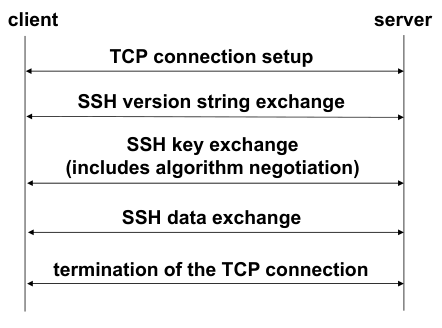
\includegraphics[width=.6\textwidth]{img/SSH layer protocol.png}
  \caption{SSH Transport Layer Protocol}
  \label{fig:ssh-layer-protocol}
\end{figure}
\subsubsection{Binary Packet Protocol}
All packets that follow the version string exchange is sent using the
Binary Packet Protocol, which is roughly the basic unit on
transmission. Every message in this kind of packet is sent as a
sequence of bytes.
\begin{figure}[h]
  \centering
  \includegraphics[width=.6\textwidth]{img/SSH bynary packet
  protocol.png}
  \caption{Binary Packet Protocol}
\end{figure}
The Binary Packet Protocol is pretty simple, it consists of:
\begin{itemize}
  \item the \textbf{length} of the \textbf{packet} (4 bytes), which
    does not include the MAC and the packet length field itself
  \item the \textbf{padding length} (1 byte), which is the length of
    the random padding field
  \item the \textbf{payload}, which may be compressed. Its size is the
    length of the packet minus the length of the length field minus 1
    (for the padding length field), up to a maximum uncompressed size
    of 32768 bytes(32KB)
  \item the \textbf{random padding}, minimum 4 bytes, up to the entire
    size of one block, and random to add confusion to the packet
  \item the \textbf{MAC}, computed over the clear text packet and the
    implicit sequence number
\end{itemize}
The first 4 fields are encrypted.

\subsubsection{Key exchange}
Another essential part of the SSH protocol is the key exchange, which 
is used to established the keys and to negotiate the algorithms to
been used.\\
One peculiarity of the SSH protocol is that the algorithms used are
selected based on directionality, which means that it is possible to
use different algorithms for the client-to-server and server-to-client
communication.\\
SSH-2 allows to select the key exchange function as well as the hash
algorithm to be used in the key derivation function. 
\begin{boxH}
  This means that the two parties have \textit{"full"} control over 
  the algorithms to be used(if supported).
\end{boxH}
  
Another interesting aspect of the protocol is that, as it was proposed
as an alternative to the Telnet protocol, it included negotiation of
the language to be used, because of the text-only nature of the 
protocol.\\
The last field of the key exchange(first key exchange packet follows)
contains an attempt to guess the agreed key exchange algorithm.\\
It contains the following fields:
\begin{itemize}
    \item SSH\_MSG\_KEXINIT
    \item cookie (16 random bytes)
    \item kex\_algorithms
      \begin{itemize}
        \item eg:diffie-hellman-group1-sha1, ecdh-sha2-OID\_of\_curve
      \end{itemize}
    \item server\_host\_key\_algorithms: used for the server authentication
      \begin{itemize}
        \item eg:ssh-rsa, ssh-dss, ecdsa-sha2-NISTP256
      \end{itemize}
    \item encryption\_algorithms\_client\_to\_server, \dots server\_to\_client
      \begin{itemize}
        \item aes-128-cbc, aes-256-ctr, aead\_aes\_128\_gcm
      \end{itemize}
    \item mac\_algorithms\_client\_to\_server, \dots server\_to\_client
      \begin{itemize}
        \item hmac-sha1, hmac-sha2-256, aead\_aes\_128\_gcm
      \end{itemize}
    \item compression\_algorithms\_client\_to\_server, \dots server\_to\_client
      \begin{itemize}
        \item none, zlib
      \end{itemize}
    \item languages\_client\_to\_server, \dots server\_to\_client
    \item first\_kex\_packet\_follows (flag)
\end{itemize}
Keep in mind that because of the negotiation of the protocols to be
used, SSH is potentially vulnerable to downgrade attacks.
\begin{boxH}
  A complete list of the supported algorithms can be found
  \href{https://www.iana.org/assignments/ssh-parameters/ssh-parameters.xhtml}{\textbf{here}}
\end{boxH}

\subsubsection{Diffie-Hellman key agreement}
This is also an \textbf{implicit authentication} of the server, due to
the fact that the server can compute the correct premaster secret
using the private key.\\
In this phase the client generates a random number $x$ and computes
$e=g^x \mod p$ and sends it to the server. The server generates a
random number $y$ and computes $f=g^y \mod p$ and sends it to the
client. At this point the key $K$ has been established. The server
computes the \textbf{exchange hash} $H$ over many fields(which makes
it basically a keyed digest): 
\begin{itemize}
  \item the client version string
  \item the server version string
  \item the client's KEXINIT message
  \item the server's KEXINIT message
  \item the shared secret $K$
  \item the exchange value $f$
  \item the exchange value $e$
  \item the host public key
\end{itemize}
and signs it with its private key to generate the signature $sigH$.\\
Those two values, together with the host public key in a raw format,
are sent to the client, which verifies the signature and computes the
same hash value. Notice that because the public key is sent in a raw 
format, the client must have a copy of the server's public key stored 
locally, and this is one of the major attack vectors of SSH.\\
Notice also that, because many algorithms need an initialization
vector, which is computed using an hash algorithm over $H$, which
makes it a keyed digest, again.


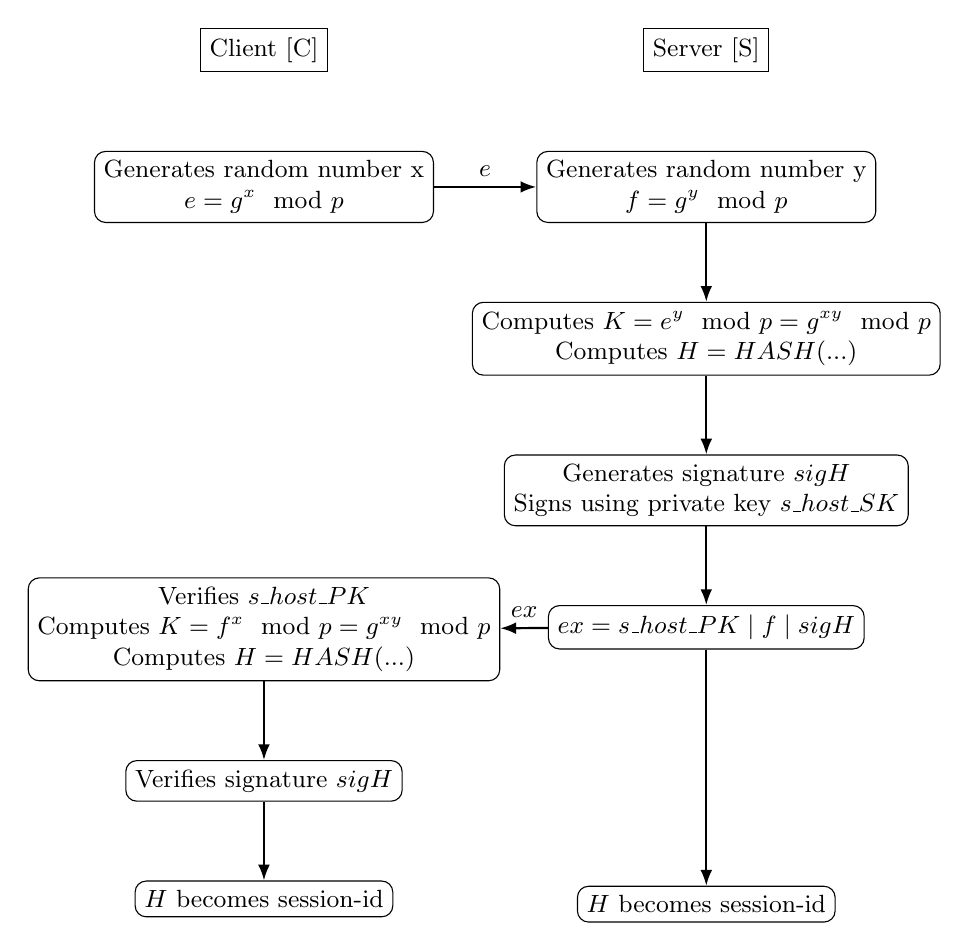
\begin{tikzpicture}[node distance=4cm, auto]
    % Define styles
    \tikzset{
        every node/.style={font=\small},
        process/.style={rectangle, draw, text centered, minimum height=1.5em, font=\small},
        data/.style={rectangle, draw, rounded corners, align=center, font=\small},
        arrow/.style={-{Latex[length=2mm]}, thick}
    }

    % Nodes for client (C) and server (S)
    \node (C) [process] {Client [C]};
    \node (S) [process, right=4cm of C] {Server [S]};

    % Client side steps
    \node (C1) [data, below=1cm of C] {Generates random number x\\$e = g^x \mod p$};
    \node (C3) [data, below=4.5cm of C1] {Verifies $s\_host\_PK$\\Computes $K = f^x \mod p = g^{xy} \mod p$\\Computes $H = HASH(...)$};
    \node (C4) [data, below=1cm of C3] {Verifies signature $sigH$};
    \node (C5) [data, below=1cm of C4] {$H$ becomes session-id};

    % Server side steps
    \node (S1) [data, below=1cm of S] {Generates random number y\\$f = g^y \mod p$};
    \node (S2) [data, below=1cm of S1] {Computes $K = e^y \mod p = g^{xy} \mod p$\\Computes $H = HASH(...)$};
    \node (S3) [data, below=1cm of S2] {Generates signature $sigH$\\Signs using private key $s\_host\_SK$};
    \node (S4) [data, below=1cm of S3] {$ex=s\_host\_PK \mid f \mid sigH$};
    \node (S5) [data, below=3cm of S4] {$H$ becomes session-id};

    % Arrows between nodes
    \draw [arrow] (C1) -- (S1) node[midway, above] {$e$};
    \draw [arrow] (S1) -- (S2);
    \draw [arrow] (S2) -- (S3);
    \draw [arrow] (S3) -- (S4);
    \draw [arrow] (S4) -- (C3) node[midway, above] {$ex$};
    \draw [arrow] (C3) -- (C4);
    \draw [arrow] (C4) -- (C5);
    \draw [arrow] (S4) -- (S5);

\end{tikzpicture}

\subsubsection{Key derivation}
Many keyed digest require a initialization vector.\\
Starting with those exchanged values, if there is any kind of algorithm that requires an IV (nearly all), then the
initial IV is:
\begin{itemize}
    \item From client to server: 
    $\text{HASH}(K \parallel H \parallel \text{"A"} \parallel \text{session\_id})$, where $K$ is the key that has been negotiated and "A" is simply a letter.
    
    \item From server to client: 
    $\text{HASH}(K \parallel H \parallel \text{"B"} \parallel \text{session\_id})$.
\end{itemize}

The encryption key is generated as follows:

\begin{itemize}
    \item From client to server: 
    $\text{HASH}(K \parallel H \parallel \text{"C"} \parallel \text{session\_id})$.
    
    \item From server to client: 
    $\text{HASH}(K \parallel H \parallel \text{"D"} \parallel \text{session\_id})$.
\end{itemize}

The integrity key:

\begin{itemize}
    \item From client to server: 
    $\text{HASH}(K \parallel H \parallel \text{"E"} \parallel \text{session\_id})$.
    
    \item From server to client: 
    $\text{HASH}(K \parallel H \parallel \text{"F"} \parallel \text{session\_id})$.
\end{itemize}

The HASH algorithm is the one used to create all these keys, and this could be a weak point because it would
be much better to generate keys using a KDF (Key Derivation Function).

\subsection{Encryption}
Encryption is compulsory in SSH, which algorithms are negotiated
during the key exchange.\\
The supported algorithms are:
\begin{itemize}
  \item (required for backward compatibility) 3des-cbc (w/ three keys,
    i.e. 168 bit key)
  \item(recommended) aes128-cbc
  \item(optional) blowfish-cbc, twofish256-cbc, twofish192-cbc,
    twofish128-cbc, aes256-cbc, aes192-cbc, serpent256-cbc,
    serpent192-cbc, serpent128-cbc, arcfour, idea-cbc, cast128-cbc,
    none
\end{itemize}
The key and initialization vector needed are established during the
key exchange and all packets sent in one direction is a single data
stream, meaning that the first packet sent has got an initialization
vector, which is the one that was created with the key derivation
function. But in the following ones, the IV is passed in the packet 
from the end of one to the beginning of the next one. In fact, there
are two cases:
\begin{itemize}
  \item if \textbf{CBC mode} is used, the IV for next packet is the
    last encrypted block of the previous packet
  \item if \textbf{CTR mode} is used, the IV for the next packet is
    the incremented value of the last IV
\end{itemize}

\subsection{MAC}
The MAC algorithm and the key are negotiated during the key exchange
and they can be different in each direction.\\
The basic set of algorithms are:
\begin{itemize}
  \item hmac-sha1 (required for backward compatibility) [key length =
    160-bit]
  \item hmac-sha1-96 (recomm) [ key length = 160-bit]
  \item hmac-md5 (opt) [key length = 128-bit]
  \item hmac-md5-96 (opt) [key length = 128-bit]
\end{itemize}
\begin{boxH}
  The mac is computed using the key for the right direction over the
  sequence number concatenated with the packet in clear text.
\end{boxH}
The sequence number is implicit, as in TLS, and its possible because 
of TCP. It is represented as a 32-bit unsigned integer, which is 
incremented by one for each packet sent.\\
This value is never reset, even if keys and algorithms are
re-negotiated, which means that when the maximum value is reached, the
channel has to be reset.
\subsection{Peer authentication}
The \textbf{server} is authenticated using an \textbf{asymmetric
challenge-response} mechanism, which requires and explicit server
signature of the key exchange hash $H$. (The challenge is implicit,
the signature is implicit).\\
The client locally stores the public keys of the server, which are
usually stored in the \texttt{known\_hosts} file in the \texttt{.ssh}
directory.\\
When connecting to a server not listed in that file, the client is
asked to store the public key of the server in the file, following a 
\textbf{TOFU} (Trust On First Use) policy.\\
Because of this, a good practice is to protect the
\texttt{known\_hosts} file for authentication and integrity, and to
periodic audit/review all the known\_hosts files to quickly detect
added/deleted hosts or changed keys.\\
Client authentication can be performed by two methods. The first one
is based on \textbf{credentials}(username and password), which are
exchanged only after the protected channel is established. This method
protects against sniffing attacks, but not other ones like password
guessing.\\
The second method is based on \textbf{asymmetric challenge-response}.
In that case, the server must locally store the public keys
of the users allowed to connect, typically in the
\texttt{authorized\_keys} file in the \texttt{.ssh} directory.\\
As per the server authentication process, as a good practice, the
\texttt{authorized\_keys} file should be protected for authentication 
and integrity, and periodically audited/reviewed to quickly detect 
added/deleted keys or changed keys.
\section{Port forwarding}
We already mentioned that SSH can act as a site-to-site VPN, but
rather than creating a general purpose VPN, SSH can be used to perform 
\textbf{port forwarding} or \textbf{tunneling}.
\begin{boxH}
  Port forwarding is a technique that allows to forward unprotected
  TCP traffic through a secure SSH channel.
\end{boxH}
This allows to secure unprotected service like POP3, SMTP or HTTP
while also allowing the application to perform their normal
authentication over an encrypted channel.\\
There are two types of port forwarding, \textbf{local} and
\textbf{remote}, but both use the Connection Protocol to encapsulate a
TCP channel inside a SSH one.
\subsection{Local port forwarding}
The concert of local port forwarding is to forward a local port to a 
remote one, which means that the client listens on a local port and 
forwards the traffic to a remote port.\\
For example, let's suppose to be behind a firewall that blocks access
to an external mail server because only secure traffic is permitted.
An SSH tunnel can be created to forward the local port 110 to the
remote port 25 using the following command:
  \begin{minted}{bash}
    ssh -L 1234:mail_server:25 user@ssh_server
  \end{minted}
the traffic to port 1234 on the (internal) client will be forwarded to
port 25 on the mail\_server by using a tunnel to the (external)
ssh\_server.\\
The firewall will see the traffic as SSH traffic, but the user has
still to configure the mail user agent to use the local port 1234 to 
connect as the outgoing mail server.

\begin{figure}[H]
  \centering
  \begin{subfigure}{.5\textwidth}
    \centering
    \includegraphics[width=.8\linewidth]{img/SHH local port forwarding
    1.png}
  \end{subfigure}%
  \begin{subfigure}{.5\textwidth}
    \centering
    \includegraphics[width=.8\linewidth]{img/SSH local port forwarding
    2.png}
  \end{subfigure}

\end{figure}

\subsection{Remote port forwarding}
Remote port forwarding is the opposite of local port forwarding, which
means that the client listens on a remote port and forwards the 
traffic to a local port.\\
For example, let's suppose to have a web server on a local machine
that is behind a firewall, and the user wants to make it available to 
the public internet. The user can create a tunnel to the remote 
machine with the following command:
  \begin{minted}{bash}
    ssh -R 8000:localhost:80 user@ssh_server
  \end{minted}
The traffic to port 8000 on the remote machine will be forwarded to 
port 80 on the local machine.\\
The user can now access the web server on the local machine by 
connecting to the remote machine on port 8000.

\begin{figure}[H]
  \centering
  \includegraphics[width=.6\textwidth]{img/SSH remote port
  forwarding.png}
\end{figure}

\subsection{Causes of insecurity}
In general, the biggest causes of insecurity for SSH are direct trust
in the public keys. In fact, x.509 certificates are not used, but some
commercial SSH implementations support them and openSSH has SSH 
certificates, which are a different thing.\\
Furthermore, blindly trusting the public keys can lead to a MITM 
attack. The server could also have a weak platform security(worms,
malicious software, rootkits, etc.) as well as the client (malware,
keyloggers, etc.).\\
One last point is that any connection to a local forwarded port will
be tunneled, even if coming from another node. This is undesirable, as
such it is recommended to specify the binding address when creating a
tunnel:
\begin{minted}{bash}
  ssh -L 127.0.0.1:1234:mail_server:25 user@ssh_server
\end{minted}

\chapter{The X.509 standard and PKI}
We will now discuss the X.509 standard and Public Key Infrastructure 
(PKI), which is widelly adopted for public key certification.
\section{Public-key certificate (PKC)}
Lets begin with a definition:
\begin{boxH}
  A \textbf{public-key certificate} is a \textbf{data structure} to securely
  bind a public key to some attributes.
\end{boxH}
A PKC is said to "securely bind" a public key to some attributes
because it is signed by a trusted entity, the \textbf{Certification
Authority}, but other techniques for certification exists (e.g.
blockchain, direct trust and personal signature).\\
The attributes in the certificate are those employed in the
transaction being protected by the PKC, which are difficult to decide
a-priori without knowing the context: for example one attribute could
be an email address associated with the entity, which may not be valid
for all the transactions.\\
PKC are most important to achieve \textbf{non-repudiation}, many
certificates have legal value, and \textbf{digital signature} in a
secure way.\\
\begin{boxH}
  Keep in mind that a PKC is the complement of a corresponding
  \textbf{personal private key}, which is kept secret by the entity.
\end{boxH}
Which means that if the private key is compromised, the PKC is 
compromised as well.
\subsection{Key Generation in Public Key Cryptography (PKC)}

Key generation in public key cryptography (PKC) involves complex
algorithms and often relies on random number generators (RNGs) to
ensure strong, unpredictable keys. Once a key is generated, the
private key must be securely protected in various contexts:

\begin{itemize}
  \item \textbf{Storage}: The private key needs to be securely
    stored to prevent unauthorized access.
  \item \textbf{Usage}: The private key must also be protected when
    being used, as it could be exposed during operations in the CPU as
    it is used in clear text.
  \item \textbf{Software Application}: In software environments
    (e.g., web browsers), the trustworthiness of the computing
    platform must be considered, as it may be vulnerable to malware
    or weak implementations. This is true both for the context of
    key generation and use.
  \item \textbf{Dedicated Hardware}: Storing and using keys in
    dedicated hardware, such as a smart card, offers enhanced
    protection but comes with limitations in terms of algorithm
    updates or vulnerability patching( which may be difficult or
    even impossible). For example many old smart cards use 1024-bit 
    RSA keys, which are considered insecure today.
  \item \textbf{Key Injection}: Keys may be generated in software
    and injected into hardware devices, a process that can be useful
    for key recovery, but should be restricted to encryption keys to
    maintain security and ensure non repudiation. This is most
    important for the private key. 
\end{itemize}

PKC key management requires careful consideration of both security and
operational challenges, especially when dealing with long-term
security mechanisms.

\subsection{Certification architecture}

In Public Key Infrastructure (PKI), several key entities are
responsible for managing the lifecycle of Public Key Certificates
(PKCs):

\begin{itemize}
  \item \textbf{Certification Authority (CA)}: The CA is responsible
    for generating and revoking PKCs. It also publishes PKCs and
    maintains information about their status, such as whether they
    are valid or revoked, or even suspended.
  \item \textbf{Registration Authority (RA)}: The RA plays a
    critical role in verifying the claimed identity and attributes
    of a certificate requestor. It authorizes the issuance or
    revocation of PKCs but does not generate them itself.
  \item \textbf{Validation Authority (VA)}: The VA provides services
    that allow third parties to verify the validity status of a PKC,
    because some responsibilities or the RA may be delegated to it.
    This may involve downloading Certificate Revocation Lists (CRLs)
    or querying an Online Certificate Status Protocol (OCSP)
    responder to check the certificate's status in real-time.
  \item \textbf{Revocation Authority}: Although not an official
    term, this role may be assigned to either the RA or CA. The
    revocation authority is delegated to revoke certificates, often
    on a more urgent basis than their issuance (they are available
    most of the time), ensuring that compromised or invalid
    certificates are promptly rendered unusable.
\end{itemize}

These entities work together to ensure the security and
trustworthiness of PKC-based systems by handling key tasks such as
certificate issuance, verification, and revocation.

\subsection{Certificate generation}
The general
When an actor want to generate a certificate, it must first generate a 
key pair (public and private key). The private key is stored locally
and protected(encrypted) as good as possible, while the public key 
is sent to the CA with some attributes that help identify the actor.\\
The CA requires that the attributes are both correct and are
associated actually with the entity that is in control of the private
key, which requires authentication of the actor. For that purpose, if
the entity is a human it is usually required to go physically to the 
CA, even if in some cases a video call may be enough, with the 
requirement of showing a valid ID.\\
The Registration Authority will verify the attributes and the 
identity of the actor, and if everything is correct, it will send a 
message to the CA to generate the certificate.\\
At this point the CA generates the certificate, signs it with its 
private key and sends it back to the actor while also storing it in 
its repository.\\
As you may noticed, the verification is only on the attributes, and
not of the possession of the private key, which will be discussed
later.

\begin{figure}[h]
  \centering
  \includegraphics[width=0.8\textwidth]{img/x509 certificate
  generation.png}
  \caption{Certificate generation}
\end{figure}

\subsubsection{Another certificate generation architecture}

In addition to what just discussed, alternative architectures for
certificate generation exist:

\begin{itemize}
  \item \textbf{Key Pair Generation by RA}: In some architectures, the
    Registration Authority (RA) generates the key pair on behalf of
    the user, obtains the Public Key Certificate (PKC), and securely
    distributes the key pair and certificate to the user via a
    secure device, such as a smart card. This approach is often used
    in large companies where the employees are already known to the
    organization.

  \item \textbf{User Authentication via Code}: Another common method
    involves the user visiting the RA to obtain a code that can be
    used to authenticate their certificate request to the
    Certification Authority (CA). The code is typically calculated
    as a Message Authentication Code (MAC) using the shared secret
    key between the RA and CA:

    \[
      \text{code} = \text{MAC}(K, ID)
    \]

    where \(K\) is a shared secret key between the RA and CA, and
    \(ID\) is the user's identity. The user then submits this code to
    the CA to validate the certificate request.
\end{itemize}

These alternative methods provide flexibility for organizations with
different security needs, allowing for centralized key generation and
secure certificate distribution.

\section{X.509 certificates}

X.509 is an ITU-T (international telecommunication unit body) standard
that defines the format of public key certificates used to verify the
identity of a key owner in cryptographic systems. X509 was developed
as a certification technology to protect the x500 directory service,
and has undergone several versions:

\begin{itemize}
  \item \textbf{v1 (1988)}: The initial version of the standard.
  \item \textbf{v2 (1993)}: A minor update with small improvements.
  \item \textbf{v3 (1996)}: Added extensions and introduced version
    1 of the attribute certificate.
  \item \textbf{v3 (2001)}: Further enhancements, including version
    2 of the attribute certificate, which are not used anymore.
\end{itemize}

X.509 is part of the larger X.500 standard for directory services,
often referred to as "white pages," which are used for managing
information about entities in a structured way(directory services).
X.509 provides a solution to the problem of securely identifying the
owner of a cryptographic key.

The certificates and their structures are defined using \textbf{ASN.1}
(Abstract Syntax Notation One), a standard interface for defining data
structures exchanged in networking environments in a neutral and 
platform-independent way. 

\subsection{PKC Scope}
A Public Key Certificate (PKC) contains information that uniquely
associates a cryptographic key with an entity. This binding between
the key and the entity is ensured by a \textbf{Trusted Third Party
(TTP)}, typically referred to as a Certification Authority (CA), which
digitally signs each certificate to guarantee its authenticity.\\

The liability associated with a PKC may be restricted to specific
applications or purposes, as outlined in the CA's certification
policy. This policy defines the intended usage and limits the scope of
the certificate, ensuring it is applied within the proper legal and
technical contexts.

\subsection{Certificate Policy (CP) and Certification Practice
Statement (CPS)}

According to RFC-3647, "Internet X.509 Public Key Infrastructure
Certificate Policy and Certification Practices Framework," both the
Certificate Policy (CP) and Certification Practice Statement (CPS)
play key roles in defining the use and management of Public Key
Certificates (PKCs):

\begin{itemize}
  \item \textbf{Certificate Policy (CP)}: A CP is a named set of rules
    that defines the applicability of a PKC to a specific community
    or class of applications with common security requirements. It
    establishes the minimum requirements for the issuance and
    management of certificates and can be followed by multiple
    Certification Authorities (CAs). For example, a government CP
    may apply to all certification providers issuing certificates
    for official use.

  \item \textbf{Certification Practice Statement (CPS)}: A CPS outlines
    the specific practices that a CA follows when issuing PKCs.
    While a CP specifies the general rules, the CPS provides
    detailed implementation procedures. Each CA develops its own
    CPS, which is tailored to its operations and describes how it
    meets the requirements set forth in the CP.
\end{itemize}

\subsection{X.500 Directory Service}

The X.500 directory service was the first system to use X.509v1
certificates. It aimed to manage information about people and entities
in a network. However, this early setup had three big issues:

\begin{itemize}
  \item \textbf{No Guarantees on the CA's Quality}: There weren't
    clear rules or policies to ensure that Certification Authorities
    (CAs) were reliable or trustworthy. People just had to trust the
    CA, which caused concern over the security of the certificates.

  \item \textbf{Lack of a proper X.500 Infrastructure}: Even though
    certificates were supposed to be stored in X.500 directories, the
    infrastructure to do this was never fully implemented worldwide.
    This made it tough to access certificates when needed.

  \item \textbf{Hard to Establish Certification Paths}: It was
    difficult to connect two users with certificates issued by
    different CAs because the relationships between CAs weren’t
    well-defined. With each CA running its own domain, figuring out
    how to establish a secure connection between users from different
    domains was tricky.
\end{itemize}

These issues slowed down the adoption of X.500 and made it clear that
better systems were needed for managing certificates.

\subsubsection{Fixing X.509v1 Problems}

To solve these problems, X.509v1 was updated with a couple of key
changes:

\begin{itemize}
  \item \textbf{Move the semantics Outside the Certificate}: Instead of
    relying on the certificate itself to define its semantics, they
    decided to put that responsibility on the application or some
    external system. This approach was used in things like RFC-1422
    (PEM), where the application takes care of interpreting the
    certificate.

  \item \textbf{Make Certificates More Flexible}: The original X.509v1
    certificates were pretty limited: they only had an identifier and a
    key. With X.509v3, they added more fields and options to make
    certificates more flexible and useful for a variety of purposes.
    This allowed them to handle a wider range of security scenarios.
\end{itemize}

These updates helped fix the early issues and set the stage for
broader adoption of the improved X.509v3 certificates.

\subsection{RFC-1422}
RFC-1422 tried to fix some of the problems with the early X.500
systems by proposing a worldwide certification hierarchy. The plan was
to have one main CA at the top: the \textbf{IPRA} (Internet Policy
Registration Authority). This CA would be responsible for setting the
rules and policies for all other CAs in the system, ensuring that
everyone followed the same security practices.\\
Instead of directly issuing certificates to lower-level CAs, the IPRA
would issue certificates to \textbf{Policy Certification Authorities
(PCAs)}.\\
The IPRA oversaw the entire structure and laid out specific
roles for different types of Certification Authorities (CAs) to manage
and enforce certificate policies:

\begin{itemize}
  \item \textbf{Policy Certification Authority (PCA)}: PCAs were
    responsible for setting and enforcing the policies that governed
    how certificates were issued. They made sure that the CAs under
    them followed the right security practices.
  
  \item \textbf{Name Subordination}: CAs had to issue certificates
    within a defined part of the naming structure, ensuring a
    consistent and organized system. For example:
  \begin{itemize}
      \item \textbf{CA n.1}: C=IT (country-level CA for Italy)
      \item \textbf{CA n.2}: C=IT, O=Politecnico di Torino (CA for an
        organization within Italy)
  \end{itemize}
\end{itemize}


 However, this system wasn’t without flaws—it
was still based on geographic hierarchies, which didn’t always match
the needs of modern, global organizations.

The IPRA was established, and four PCAs were created under it. One of
these PCAs was designated as \textbf{high assurance}, meaning it had
to carry out stricter checks before issuing certificates. For
instance, BBN, a company heavily involved with the U.S. military,
might require things like fingerprints or even DNA tests to verify
identities.

In contrast, \textbf{mid-level assurance} certificates, like those
issued by universities such as MIT, required less rigorous
checks—maybe just showing a passport. MIT could even set up its own
subordinate CAs, like one for the Laboratory for Computer Science, to
handle its internal certificate needs.

What’s interesting is how different cultural practices shaped the
certification process. In the U.S., where people don’t generally carry
ID cards, \textbf{residential certification authorities} were used. If
you wanted to open a bank account, for example, you might have to show
an electricity bill to prove your address. While this seems strange in
countries with formal ID systems, in the U.S., it was a necessity.

Finally, there were \textbf{persona certificates}, which allowed for
anonymous certificates. These were for users who didn’t want to reveal
their identity but still needed secure communications. For example,
you could be “anonymous user number 95.” Even though no one knew who
you were, the security of your communication was still guaranteed.

\begin{figure}[h]
  \centering
  \includegraphics[width=0.8\textwidth]{img/x509 internet per
  hierarchy.png}

  \caption{Internet PEM hierarchy (RFC-1422)}
\end{figure}

Unfortunately, this system was a complete failure for several reasons:

\begin{itemize}
  \item The hierarchical structure severely limited flexibility, much
    like the issues we saw with X.500. For international companies,
    this rigid hierarchy simply didn't work.

  \item Name subordination imposed additional restrictions. You
    couldn't just assign any name—you had to follow the strict
    hierarchy, which wasn't always practical.

  \item The use of the PCA concept lacked flexibility, especially in
    commercial settings. Instead of automating the process, a human
    operator was needed to check if the requester was following the
    policy. This made the system cumbersome and inefficient for
    businesses.

  \item Lastly, the biggest issue was trust. Where would the IPRA be
    placed? Naturally, the U.S. wanted it, but other countries, like
    Russia, China, or even Japan, wanted control as well. No one
    trusted a single country to sit at the top of the hierarchy,
    fearing the possibility of a fake hierarchy being created. As a
    result, the experiment collapsed. It briefly existed, primarily
    used by the United States, but it never gained global traction.
\end{itemize}

\section{X.509 Version 3}

X.509 Version 3 is a standard that was finalized in June 1996 through
a collaborative effort between ISO, ITU, and the IETF, with the goal
of making certificates suitable for internet applications. This
version consolidated all the necessary updates to certificates and
Certificate Revocation Lists (CRLs) into a single document. Earlier
versions of X.509 (v1 and v2) relied on external semantics, such as
the failed attempt with the Internet PEM hierarchy, which proved
unsuccessful. X.509v3 addressed these shortcomings by ensuring
certificates would be useful for internet applications, particularly
as OSI applications became mostly obsolete.\\
Key features of X.509 Version 3 include:

\begin{itemize}
  \item \textbf{Types of Extensions}:
    \begin{itemize}
      \item \textbf{Public Extensions}: These are defined by the
        standard and made publicly available for anyone to use.
        Because they are standardized, any system or application
        should be able to understand and process them.
      \item \textbf{Private Extensions}: These are tailored to
        specific user communities and are not publicly available. If a
        system does not understand a private extension, it will treat
        it as a binary blob and discard it. Private extensions are
        crucial for certain organizations that require custom
        functionality.
    \end{itemize}
    
    The introduction of extensions is a major improvement in X.509v3,
    adding flexibility without changing the fundamental structure of
    the certificate (which remains the same as in X.509v1). Extensions
    are contained within a small field but open up a wide range of
    possibilities. Public extensions ensure standard compatibility,
    while private extensions allow customization specific to
    organizations.

  \item \textbf{Certificate Profile}: This refers to a set of
    extensions tailored for a specific purpose or application,
    ensuring that certificates meet particular requirements. For
    example, RFC 5280, titled "Internet X.509 Public Key
    Infrastructure Certificate and Certificate Revocation List (CRL)
    Profile," provides guidelines on how X.509 certificates and CRLs
    should be structured for protecting internet applications.
    Certificate profiles are important because they dictate how
    certificates should be used for different scenarios, ensuring
    consistency and security.
\end{itemize}


\subsection{Base syntax}

The base syntax of an X.509 certificate is defined as follows:

\begin{verbatim}
Certificate ::= SEQUENCE {
    signatureAlgorithm AlgorithmIdentifier,
    tbsCertificate TBSCertificate,
    signatureValue BIT STRING
}

TBSCertificate ::= SEQUENCE {
    version [0] Version DEFAULT v1,
    serialNumber CertificateSerialNumber,
    signature AlgorithmIdentifier,
    issuer Name,
    validity Validity,
    subject Name,
    subjectPublicKeyInfo SubjectPublicKeyInfo,
    issuerUniqueID [1] IMPLICIT UniqueIdentifier OPTIONAL,
        -- if present, version must be v2 or v3
    subjectUniqueID [2] IMPLICIT UniqueIdentifier OPTIONAL,
        -- if present, version must be v2 or v3
    extensions [3] Extensions OPTIONAL
        -- if present, version must be v3
}
\end{verbatim}

This abstract notation outlines the basic structure of the
certificate. The \texttt{Certificate} is defined as a sequence, which
is a data structure that includes several fields. The first field,
\texttt{signatureAlgorithm}, is the algorithm identifier used by the
Certificate Authority (CA) to sign the certificate. 

Next, the \texttt{tbsCertificate} (to be signed certificate) is of
type \texttt{TBSCertificate}, which contains the main information that
needs to be signed. Finally, the \texttt{signatureValue} is a bit
string that holds the actual signature.

The \texttt{TBSCertificate} is again defined as a sequence, starting
with the \texttt{version} field, which begins numbering with zero,
indicating version 1. For version 3, this field has a value of two.
Following that, we have the \texttt{serialNumber} of the certificate
and the \texttt{signature} algorithm identifier. 

You may wonder why the signature algorithm appears twice—once
externally and once within the \texttt{TBSCertificate}. The external
algorithm identifier is crucial for verifying the signature; without
knowing the algorithm, you cannot validate the signature value. Having
it specified internally helps ensure that the signature algorithm used
for verification matches the algorithm used for signing. If they
differ, it's a red flag, indicating that the certificate should not be
trusted.

The \texttt{issuer} field identifies the certification authority by
name, and the \texttt{validity} field specifies the validity period of
the certificate. The \texttt{subject} is identified by its name, and
the \texttt{subjectPublicKeyInfo} field contains both the algorithm
and the actual public key of the subject.

In addition, versions 2 and 3 introduce optional unique identifiers
for both the issuer and subject, though these identifiers are rarely
used today. Finally, the \texttt{extensions} field, which is optional,
must be present for certificates of version 3, as earlier versions do
not support extensions.


\subsection{Critical Extensions}

In the context of X.509 certificates, extensions can be classified as
critical or non-critical, each affecting the certificate verification
process differently:

\begin{itemize}
  \item \textbf{Critical Extensions}: If a certificate contains an
    unrecognized critical extension, it \textbf{MUST} be rejected
    during the verification process. This ensures that any essential
    information required for proper validation is recognized and
    handled appropriately.

  \item \textbf{Non-Critical Extensions}: Conversely, a non-critical
    extension \textbf{MAY} be ignored if it is unrecognized. This
    allows flexibility in certificate processing, as non-critical
    information does not impede the overall verification of the
    certificate.
\end{itemize}

The responsibility for handling these extensions lies entirely with
the entity performing the verification, referred to as the
\textbf{Relying Party (RP)}. The RP must implement logic to correctly
interpret and respond to both critical and non-critical extensions in
accordance with their definitions.

\subsection{Public Extensions}

X.509 version 3 defines four classes of public extensions that enhance
the functionality and applicability of certificates:

\begin{itemize}
  \item \textbf{Key and Policy Information}: Extensions in this
    class provide additional information regarding the key usage and
    policies applicable to the certificate, guiding how the key
    should be used within specific contexts.

  \item \textbf{Certificate Subject and Certificate Issuer
    Attributes}: These extensions include attributes related to both
    the subject of the certificate (the entity that the certificate
    represents) and the issuer (the Certification Authority),
    enabling more detailed identification and classification.

  \item \textbf{Certificate Path Constraints}: These extensions
    define rules and limitations regarding the certification path,
    ensuring that certificates can only be used in certain contexts
    or under specific conditions, enhancing security within the
    certificate hierarchy.

  \item \textbf{CRL Distribution Points}: This extension indicates
    where the Certificate Revocation List (CRL) can be found,
    providing necessary information for relying parties to check the
    revocation status of the certificate efficiently.
\end{itemize}

\subsection{Key and policy information}


There are six public extensions dedicated to this purpose. 
We won't discuss all of them, but we will focus on the most important 
ones.

\subsubsection{Authority Key Identifier}

Key and policy information extensions in X.509 v3 provide crucial
details about the public keys associated with certificates. One
significant component is the \textbf{Authority Key Identifier (AKI)},
which serves the following purposes:

\begin{itemize}
  \item \textbf{Identification of the Signing Key}: The AKI identifies
    a specific public key used to sign a certificate, ensuring that
    the verification process can accurately trace the certificate's
    authenticity back to the correct authority.

  \item \textbf{Identification Methods}: The identification can be
    achieved through:
    \begin{itemize}
      \item A \textbf{key identifier}, typically represented as the
        digest (hash) of the public key of the certification authority.
      \item The combination of \textbf{issuer-name} and 
        \textbf{serial-number}, allowing a clear reference to the
        issuing CA's key.
    \end{itemize}

  \item \textbf{Usage}: The AKI is particularly useful in scenarios
    where the same CA might utilize multiple keys, such as for 
    different assurance levels, like low assurance for general use 
    and high assurance for sensitive applications.

  \item \textbf{Non-Critical Extension}: While the AKI is classified 
    as non-critical, its presence can be vital in certain 
    applications. In the professor experience, the absence of this 
    extension can lead to many applications rejecting the certificate
    as invalid.

  \item \textbf{Importance in Certificate Chains}: When an 
    application receives a certificate, it often needs to establish 
    a trust path up to a root CA. This path-building process relies 
    heavily on the AKI field. If a CA neglects to include this 
    extension, it may lead to compatibility issues with various 
    applications, despite being non-critical.
\end{itemize}

\subsubsection{Subject key identifier}
The \textbf{Subject Key Identifier} (SKI) extension serves
to identify a specific public key associated with a certificate. Key
features include:

\begin{itemize}
  \item \textbf{Identification of Public Key}: The SKI uniquely
    identifies a particular public key used in an application. This
    is especially important in scenarios where the public key may be
    updated or replaced over time.

  \item \textbf{Being Non-Critical}: The SKI is classified as a
    non-critical extension, meaning that while it provides valuable
    identification information, its absence does not necessarily
    prevent the certificate from being considered valid.
\end{itemize}
This one is usually not present in the certificate because an
identifier is already present in the certificate.
\subsubsection{Key usage}

The \textbf{Key Usage} (KU) extension specifies the application
domains in which a public key may be utilized. Key characteristics
include:

\begin{itemize}
  \item \textbf{Application Domain Identification}: The KU extension
    identifies the specific purposes for which the associated public
    key can be employed, ensuring that it is used appropriately
    within defined contexts. In case of misuse, the application may
    refuse to accept the certificate and the CA may refuse liability.

  \item \textbf{Critical or Non-Critical}: The Key Usage extension
    can be classified as either critical or non-critical:
    \begin{itemize}
      \item If marked as \textbf{critical}, the certificate may only
        be used for the specific purposes indicated in the Key Usage
        extension. Any usage outside the defined scopes would render
        the certificate invalid.
      \item If marked as \textbf{non-critical}, the certificate can
        be used more flexibly, potentially allowing usage beyond the
        defined applications without invalidating the certificate.
    \end{itemize}

  \item \textbf{Permitted Cryptographic Operations}: The following
    cryptographic operations can be defined within the Key Usage
    extension:
    \begin{itemize}
      \item \textbf{digitalSignature}: valid in the certificate of a
        user but also in the certificate of a certification authority.
      \item \textbf{nonRepudiation}: Specifically permitted for
        users (non repudiation is only for humans after all).
      \item \textbf{keyEncipherment}: Permitted for users.
      \item \textbf{dataEncipherment}: Allowing encryption of data.
      \item \textbf{keyAgreement}: Involves:
        \begin{itemize}
          \item \textbf{encipherOnly}: Restricting use to
            enciphering operations.
          \item \textbf{decipherOnly}: Restricting use to
            deciphering operations.
        \end{itemize}
      \item \textbf{keyCertSign}: Specifically permitted for
        Certificate Authorities (CAs).
      \item \textbf{cRLSign}: Also permitted for Certificate
        Authorities (CAs) for signing Certificate Revocation Lists
        (CRLs).
    \end{itemize}
\end{itemize}

\subsubsection{Private key usage period}

The \textbf{Private Key Usage Period} extension in X.509 v3 specifies the
time frame during which the associated private key may be used. Key
features include:

\begin{itemize}
  \item \textbf{Usage Period Definition}: This extension defines the
    period during which the private key can be actively utilized,
    helping to enforce time-based restrictions on key usage.

  \item \textbf{Non-Critical Extension}: The Private Key Usage
    Period extension is always classified as non-critical, meaning
    that its absence does not invalidate the certificate. However,
    the information it provides can be important for managing key
    lifecycles.

  \item \textbf{Usage Discouraged}: While this extension is
    available, its use is generally discouraged in practice.
    Organizations often prefer to manage key lifetimes through other
    means, such as regular key rotation, rather than relying on a
    specified usage period within the certificate.
\end{itemize}

\subsubsection{Certificate policies}

The \textbf{Certificate Policies} extension outlines the specific
policies that were adhered to during the issuance of the certificate
and defines the purposes for which the certificate can be utilized.
Key aspects include:

\begin{itemize}
  \item \textbf{Policy Listing}: This extension provides a
    comprehensive list of the policies that govern the certificate
    issuance process, ensuring clarity regarding its intended use.

  \item \textbf{Indication Methods}: Certificate policies can be
    indicated using various formats, including:
    \begin{itemize}
      \item \textbf{Object Identifier (OID)}: A unique identifier for
        the policy.
      \item \textbf{Uniform Resource Identifier (URI)}: A link to a
        location where the policy can be reviewed.
      \item \textbf{Text Message}: A textual description of the
        policy.
    \end{itemize}

  \item \textbf{Critical or Non-Critical}: The Certificate Policies
    extension can be classified as either critical or non-critical:
    \begin{itemize}
      \item If marked as \textbf{critical}, the certificate must only
        be used in accordance with the specified policies; otherwise,
        it may be considered invalid.
      \item If marked as \textbf{non-critical}, the certificate can be
        used more flexibly, although the policies still provide
        guidance for its intended use.
    \end{itemize}

  \item \textbf{Support for Authentication and Authorization}: The use
    of this extension can enhance not only the authentication of users
    and entities but also facilitate authorization processes,
    providing a clearer understanding of the permissible actions
    associated with the certificate.
\end{itemize}

\subsubsection{Policy mappings}

The \textbf{Policy Mappings} extension in X.509 v3 establishes a
correspondence between policies across different certification
domains. Key aspects include:

\begin{itemize}
  \item \textbf{Mapping of Policies}: This extension indicates how
    policies from one certification authority (CA) correspond to
    policies from another, facilitating interoperability and trust
    among different certificate frameworks. This can be done
    automatically, but needs human interaction to be done correctly.

  \item \textbf{Presence in CA Certificates}: The Policy Mappings
    extension is typically present only in CA certificates, allowing
    certification authorities to define and communicate
    relationships between their policies and those of other
    authorities.

  \item \textbf{Non-Critical Extension}: The Policy Mappings
    extension is classified as non-critical, meaning its absence
    does not invalidate the certificate. However, it serves as an
    important tool for enhancing the understanding and usability of
    certificates across different domains.
\end{itemize}

\subsection{Certificate subject and issuer attributes}
As previously mentioned, the X.509 v3 standard includes extensions 
that provide additional information about the subject and issuer of a 
certificate. Without this extension, the only possible names are x500
ones, which aren't really an identifier.
\subsubsection{Subject Alternative Name (SAN)}
The Subject Alternative Name (SAN) extension provides a flexible way
to identify the owner of a certificate. This extension allows the use
of various formalisms to represent the owner, including e-mail
addresses, IP addresses, and URLs.\\
Importantly, the SAN field is always considered critical when the
subject name field is empty. This means that if there is no subject
name, the SAN extension must be present to ensure proper identification
and functionality of the certificate.

\subsubsection{Issuer Alternative Name (IAN)}
The Issuer Alternative Name (IAN) extension in enables the use of
various formalisms to identify the Certificate Authority (CA) that
issued a certificate or a Certificate Revocation List (CRL). This
extension supports different identifiers such as e-mail addresses, IP
addresses, and URLs.\\
The IAN field is always considered critical when the issuer name field 
is empty. In such cases, the IAN extension must be present to ensure 
proper identification of the issuing authority.\\

It's also interesting to see what are the possible identifiers that 
can be used in the IAN field.\\
 One option is the \textbf{RFC 802 Name}, which consists 
of the standard email addresses used in internet applications. The 
\textbf{DNS Name} identifies a node by its domain name, while an 
\textbf{IP Address} identifies the node by its numerical address. 
Another alternative is the \textbf{Uniform Resource Identifier (URI)}, 
which serves as an entry point on the web. This means that on the 
same node, you could have different certificates corresponding to 
various entry points for the applications.

In addition, you can use a \textbf{Directory Name}, which can be 
formatted according to X.500 or LDAP syntax. For example, the 
LDAP of the Politecnico di Torino might be represented as 
\texttt{country=T; organization=Politecnico di Torino; organizationUnit=Department}. 
While there is no formal management of country Italy in this case, 
the syntax remains consistent. 

Moreover, \textbf{X.400 Addresses} illustrate that these identifiers 
were still in use when version 3 was developed in 1996, as there 
were gateways that transformed mail from X.400 to RFC 802 formats. 
Thus, having the certificate associated with the X.400 address 
was essential. 

Next, we have the \textbf{EDI Party Name}, which stands for 
electronic data interchange. This standard allows companies to 
avoid manual processing of data. For instance, a car manufacturer 
might need to check if a supplier has specific tires available. 
Instead of making a phone call or sending a fax or email, they 
could use EDI to make a query through a neutral language that 
facilitates data requests and responses electronically. 

EDI serves as a general standard with various implementations, such 
as EDIFACT, which Stellantis and many other car manufacturers use 
to manage the availability of necessary items, check prices, and 
place orders. The significance of EDI is reflected in the 
certificates associated with it. 

Although EDI may seem older compared to modern standards like XML or 
JSON, many companies still rely on these established systems to avoid
dealing with breaking changes that may occur.

In addition to the EDI Party Name, a \textbf{Registered ID}, 
such as a VAT number for a company or an Italian tax number for 
individuals, can also be used. This represents any official 
registered identifier for an entity. Another identifier is the 
\textbf{Unique Identifier}, which signifies a distinct identifier 
for individuals or organizations. Finally, there is the 
\textbf{Other Name} option. This should be used cautiously, as 
it lacks a well-defined structure. When using the "Other Name," 
the syntax and content definition fall to the user, making it 
non-standard and challenging to interpret.

\subsubsection{Subject Directory Attributes}

The Subject Directory Attributes extension allows for the storage of
specific directory attributes related to the owner of the certificate.
For example, the Department of Defense (DoD) utilizes this extension
to indicate attributes like "citizenship." \\
The actual usage of Subject Directory Attributes heavily depends on 
the application since there are no standard definitions for these 
attributes. This extension is classified as non-critical, meaning 
its absence does not prevent the certificate from being valid but 
may limit its utility in certain contexts.

\subsection{Certificate path constraints}
Let's now go over the chain of trust and the constraints that can be 
created in the certificate path.\\
There are three main constraints that can be set in the certificate 
path.
\subsubsection{Basic Constraints}

\begin{boxH}
  The correct term for user in the context of certificates is
  \textbf{end-entity} (EE).
\end{boxH}

\subsubsection{Basic Constraints}

The Basic Constraints extension indicates whether the subject of 
the certificate can act as a Certificate Authority (CA). The 
values for this extension are defined as follows: 

\begin{itemize}
    \item \textbf{BC=true}: This indicates that the subject 
    is a CA.
    \item \textbf{BC=false}: This indicates that the subject 
    is an End Entity (EE).
    \item Additionally, it is possible to define the maximum 
    depth of the certification tree, but only if 
    \textbf{BC=true}.
    \item This extension can be classified as either 
    critical or non-critical, though it is suggested to 
    always mark this extension as critical.
\end{itemize}


\subsubsection{Name Constraints}
The Name Constraints extension is applicable only in 
Certificate Authority (CA) certificates. This extension 
defines the space of names that can be certified by a CA 
and follows the same format as the Alternative Names.

Key points regarding Name Constraints include:

At least one specification must be provided between:
\begin{itemize}
    \item \textbf{permittedSubtree}: This serves as a 
    whitelist for names that are allowed.
    \item \textbf{excludedSubtree}: This serves as a 
    blacklist for names that are not allowed.
\end{itemize}

The whitelist is processed first, ensuring that allowed 
names take precedence. Caution is advised: An unspecified 
format in the whitelist (e.g., \texttt{directoryName}) 
is implicitly permitted. This extension can be either 
critical or non-critical, though it is important to note 
that there is no non-critical support by Apple.
\subsubsection{Policy Constraints}
The Policy Constraints extension is used by a 
Certificate Authority (CA) to specify constraints 
that may require an explicit identification by a 
policy or that inhibit policy mapping for the 
remainder of the certification path. 

This extension can be either critical or non-critical.

\subsection{CRL distribution point}

The CRL Distribution Point extension identifies the 
distribution point of the Certificate Revocation List 
(CRL) that is to be used in validating a certificate. 

The distribution point can be specified in various forms, 
including:
\begin{itemize}
    \item \textbf{Directory entry}
    \item \textbf{E-mail} or \textbf{URL}
\end{itemize}

This extension can be either critical or non-critical.

\subsection{Private Extensions}

The \textbf{Private Extensions} in X.509 v3 enable the creation of 
extensions tailored to specific user communities, allowing for 
customized applications within closed groups. 

One key aspect of private extensions is their definition. These are 
custom-defined features intended for use by particular communities 
or groups of users. This capability provides both flexibility and 
specificity in the application of certificates, allowing them to 
meet the unique needs of different organizations or use cases.

Another important consideration is the examples from the Internet 
Engineering Task Force Public Key Infrastructure (IETF-PKIX), which 
has defined three notable private extensions for the Internet user 
community. The first of these is \textbf{Subject Information Access}, 
which provides essential details on how to access data related to 
the subject of the certificate. The second extension, known as 
\textbf{Authority Information Access}, offers guidance on how to 
access information pertaining to the certificate authority, ensuring 
that users can verify and trust the source of the certificate. 
Finally, the \textbf{CA Information Access} extension supplies vital 
information for accessing resources linked to the certificate 
authority, facilitating the management and verification of 
certificates within the relevant community.
\subsubsection{Subject Information Access}

The \textbf{Subject Information Access} extension in X.509 v3 
specifies a method for obtaining additional information about the 
owner of a certificate, particularly useful when a directory 
service is not employed for certificate distribution. This 
extension allows users to retrieve extra details regarding the 
certified end entity, which can be important for verifying 
credentials or understanding the context of the certificate.

The extension typically includes a method, such as HTTP, HTTPS, 
or LDAP, which outlines the protocol to be used for accessing 
the required information. Alongside this method, it provides a 
name indicating the location or address where the information 
can be obtained. For instance, it might direct users to a 
specific web page related to the individual or point to a 
local directory entry.

It is important to note that this extension is classified as 
non-critical, meaning it serves primarily as informational. 
While it enhances the utility of the certificate by providing 
additional access methods, it does not impact the fundamental 
validation of the certificate itself.
\subsubsection{Authority Information Access}

The \textbf{Authority Information Access (AIA)} extension plays a 
crucial role in X.509 certificates, as it specifies how to access 
the information and services offered by the certificate authority 
(CA) that issued the certificate. This extension is applicable 
to any certificate, whether from a certification authority or an 
end entity.

AIA contains several important subfields that facilitate various 
functions. One key subfield is \textbf{certStatus}, which may include 
a URL for an Online Certificate Status Protocol (OCSP) responder. 
This is particularly useful for checking the real-time status of a 
certificate, complementing the Certificate Revocation List (CRL) 
distribution point. 

Additionally, AIA may provide pointers for:

\begin{itemize}
  \item \textbf{certRetrieval}: This subfield allows for the retrieval 
    of the certificate itself from a specified location.
  \item \textbf{cAPolicy}: It outlines the policies under which the CA 
    operates, offering insight into the trustworthiness of the 
    certificate.
  \item \textbf{caCerts}: This indicates where to find the CA's own 
    certificates, which is essential for building a certification 
    path.
\end{itemize}

The presence of AIA in a certificate enables users to locate 
the services provided by the CA. It acts as a guide for 
retrieving necessary information, such as following a path to 
an OCSP responder or accessing the CA's certificates. While the 
AIA extension can be classified as either critical or non-critical, 
it is typically recommended for scenarios that require real-time 
status checks or validation. This extension enhances the 
functionality of certificates by making it easier to access 
relevant information necessary for establishing trust.

\begin{figure}[h]
  \centering
  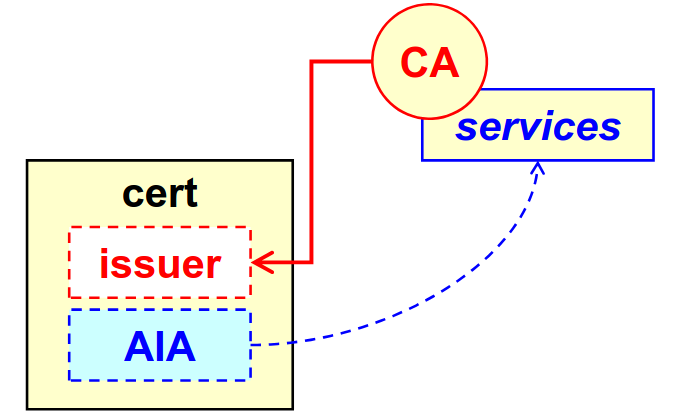
\includegraphics[width=0.5\textwidth]{img/x509 AIA.png}

  \caption{Authority Information Access (AIA) extension}
\end{figure}

\subsubsection{CA Information Access}

The \textbf{CA Information Access (CAIA)} extension serves a 
specific function in X.509 certificates, as it indicates how to 
access information and services provided by the certificate 
authority (CA) that owns the certificate. Unlike other 
extensions, CAIA is valid only within a CA certificate itself.

CAIA includes several important subfields that facilitate access 
to the CA's services, such as:
\begin{itemize}
  \item \textbf{certStatus}: This subfield may point to the status of 
    the CA's certificates, typically through an OCSP responder.
  \item \textbf{certRetrieval}: This allows for the retrieval of the 
    CA's own certificate from a designated location.
  \item \textbf{cAPolicy}: This subfield provides information on the 
    policies that govern the CA's operations, helping users 
    understand the trust model.
  \item \textbf{caCerts}: It indicates where the CA's certificates can 
    be accessed, which is vital for validating the certificate 
    chain.
\end{itemize}

The significance of CAIA lies in its role as a self-pointer for 
the CA. When you possess a CA certificate and wish to locate its 
services, CAIA provides the necessary pointers to information 
about the CA itself, including its policy, OCSP responder, and 
certificate repository. This self-referential nature distinguishes 
CAIA from other access methods, which typically point back to the 
parent CA. As with many extensions, CAIA can be classified as 
either critical or non-critical, depending on the context in 
which it is used. However, it is particularly valuable for 
establishing a complete understanding of the CA's services and 
trustworthiness.

\begin{figure}[h]
  \centering
  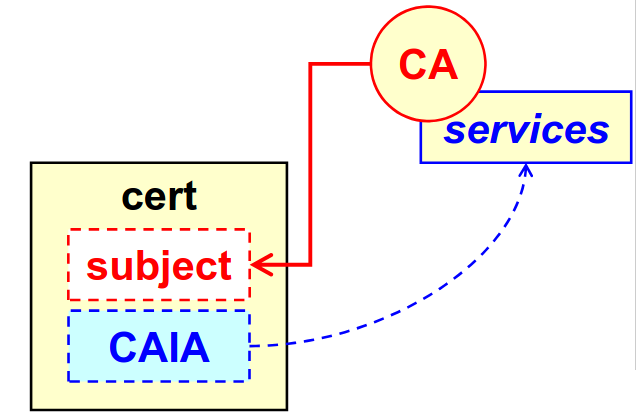
\includegraphics[width=0.5\textwidth]{img/x509 CAIA.png}

  \caption{CA Information Access (CAIA) extension}
\end{figure}

\subsubsection{RFC-2459}

The \textbf{RFC-2459} document defines a profile for the use of 
X.509v3 certificates in Internet applications, such as IPsec, TLS, 
and S/MIME. This profile was initially suggested by the Public Key 
Infrastructure (PKIX) working group to promote interoperability 
and standardization across diverse systems and protocols.

One of the key aspects of RFC-2459 is that it establishes extensions 
defined by an Object Identifier (OID), specifically using the base 
\texttt{ID-PKIX ::= 1.3.6.1.5.5.7} (which maps to 
\texttt{iso.org.dod.inet.sec.mechanisms.pkix}). OIDs ensure that 
each extension and algorithm used within the X.509 framework is 
uniquely identifiable and properly managed. For instance, PKIX 
requested an OID rooted in the U.S. Department of Defense namespace 
due to the historical origin of the internet (as DARPA Net), and 
further sub-trees were established for protocols like IPsec, TLS, 
and S/MIME.

RFC-2459 also specifies the supported algorithms that should be 
implemented to ensure secure and reliable communication. Beyond 
defining supported algorithms, it offers several implementation 
suggestions to enhance compatibility. A few examples include:
\begin{itemize}
    \item \textbf{UTC Time}: It is mandatory to include seconds 
    in time fields.
    \item \textbf{Zulu Time}: UTC time must be expressed in the 
    Zulu (Greenwich Mean Time) timezone, which avoids issues with 
    software systems that misinterpret time zones. For instance, 
    some software (notably from Microsoft) might default to local 
    time, causing inconsistencies.
    \item \textbf{Two-Digit Year Format}: Although specifying the 
    year in two digits is not recommended, when used, it should be 
    interpreted within the range of 1950-2049. After 2049, 
    certificates must switch to four-digit year formats to avoid 
    ambiguity and incompatibility issues.
\end{itemize}

By adhering to the guidelines outlined in RFC-2459, certificate 
issuers and consumers ensure proper functionality across diverse 
systems, especially in the context of internet security protocols. 
The use of standardized extensions, supported algorithms, and 
implementation details like time format further strengthens 
interoperability and the reliability of X.509 certificates.

\subsubsection{Extended Key Usage}

The \textbf{Extended Key Usage} (EKU) extension in X.509 certificates 
allows for defining specific uses of a certificate in addition to, 
or in substitution of, the standard \texttt{keyUsage} extension. 
Unlike the standard key usage, which is focused on cryptographic 
operations, EKU is oriented towards specific applications. This 
enables a certificate to be more narrowly defined for its intended 
purpose, enhancing security and clarity in certificate handling.

EKU can be used simultaneously with the standard \texttt{keyUsage} 
extension, though it is important to consider how conflicts between 
the two might be handled in practice. EKU serves to tailor 
certificates for specific tasks within certain application domains, 
which is particularly useful in environments requiring strict 
certification boundaries, such as server authentication or 
email protection.

Some of the possible values for EKU include:
\begin{itemize}
    \item \texttt{serverAuth} (\texttt{id-pkix.3.1}): This EKU 
    designates a certificate for server authentication. In cases 
    where serverAuth is used, the equivalent key usages that should 
    be enabled include Digital Signature (DS), Key Encipherment (KE), 
    and Key Agreement (KA).
    \item \texttt{clientAuth} (\texttt{id-pkix.3.2}): This EKU is 
    intended for client-side authentication and can be mapped to 
    Digital Signature (DS) and Key Agreement (KA).
    \item \texttt{codeSigning} (\texttt{id-pkix.3.3}): This EKU is 
    used for code signing, allowing developers to sign the code they 
    create. The primary associated key usage is Digital Signature 
    (DS).
    \item \texttt{emailProtection} (\texttt{id-pkix.3.4}): This EKU 
    provides a certificate for email protection. It includes Digital 
    Signature (DS), Non-Repudiation (NR), Key Encipherment (KE), and 
    Key Agreement (KA) as the relevant key usages.
    \item \texttt{timeStamping} (\texttt{id-pkix.3.8}): Used for 
    timestamping, this EKU is associated with Digital Signature (DS) 
    and Non-Repudiation (NR). Timestamping certificates are crucial 
    for certifying when a particular action, such as a signature, 
    took place.
    \item \texttt{ocspSigning} (\texttt{id-pkix.3.9}): This EKU is 
    specific to signing OCSP responses. The associated key usages 
    are Digital Signature (DS) and Non-Repudiation (NR), ensuring 
    that OCSP responses are properly authenticated.
\end{itemize}

In summary, the PKIX group developed EKU to provide more granular 
control over certificate usage within specific applications. For 
example, a certificate intended for email may only be valid for email 
protection, while another for server authentication may only serve 
that purpose. The flexibility offered by EKU allows for more precise 
security policies, tailored to the needs of individual systems or 
applications.

\subsubsection{Evolution of RFC-2459}

The evolution of \textbf{RFC-2459}, which initially defined the 
profile of X.509v3 certificates for use in Internet applications, 
reflects a series of updates and refinements to both certificate 
profiles and cryptographic algorithms.

RFC-2459 was replaced by two key documents:
\begin{itemize}
    \item \textbf{RFC-3280}: This document defines the Internet 
    profile of public key infrastructures (PKIs) based on X.509v3 
    certificates and X.509v2 certificate revocation lists (CRLs). 
    It was intended to standardize how certificates and CRLs are 
    managed and used in Internet-based PKI systems.
    \item \textbf{RFC-3279}: This document covers the algorithms 
    used in conjunction with the RFC-3280 profile, providing 
    identifiers, parameters, and encodings. It includes, and makes 
    obsolete, the earlier RFC-2528, which addressed the use of 
    the Key Exchange Algorithm (KEA).
\end{itemize}

The decision to split RFC-2459 into two separate RFCs was driven by 
the recognition that while certificate profiles tend to remain stable 
over time, cryptographic algorithms evolve more rapidly. By 
documenting algorithms separately in RFC-3279, it became easier to 
update the list of supported algorithms without needing to revise the 
entire certificate profile.

Later on, \textbf{RFC-3280} was itself obsoleted by \textbf{RFC-5280}, 
which further refined the Internet PKI profile and introduced updates 
to align with advancements in cryptographic practices and PKI 
implementation. RFC-5280 remains a foundational document in the 
definition of PKI systems used for securing Internet communication.
\subsubsection{RFC-3279 and Supported Algorithms}

\textbf{RFC-3279} specifies the algorithms that \emph{MUST} be 
supported by applications using the \textbf{RFC-3280} profile. 
It includes some older algorithms, as well as newer ones. The key 
algorithms defined in this RFC are:

\begin{itemize}
  \item \textbf{Digest algorithms:}
  \begin{itemize}
    \item MD-2, MD-5, SHA-1 (preferred)
  \end{itemize}
  \item \textbf{Algorithms for signing certificates/CRLs:}
  \begin{itemize}
    \item RSA, DSA, \underline{ECDSA (Elliptic Curve DSA)}
  \end{itemize}
  \item \textbf{Subject public key algorithms (SubjectPublicKeyInfo):}
  \begin{itemize}
    \item RSA, DSA, \underline{KEA}(a variant of Diffie-Hellman), DH
      (Diffie-Hellman), \underline{ECDSA}, \underline{ECDH (Elliptic
      Curve Diffie-Hellman)}
  \end{itemize}
\end{itemize}

The underlined algorithms were introduced in \textbf{RFC-3279} in 
comparison to \textbf{RFC-2459}. One important point is that RFC-3279 
permits the use of legacy algorithms, though they are not recommended 
(e.g., SHA-1 is preferred for digest, and RSA/DSA for certificate 
signing, with ECDSA added for more modern use). 

Once the basic definitions are set, optional algorithms can be defined. 
Notably:

\begin{itemize}
  \item \textbf{RFC-4055:} Adds better specifications for signatures, 
    including the Probabilistic Signature Scheme (PSS), Optimal 
    Asymmetric Encryption Padding (OAEP), and SHA-2 for digest 
    computation.
  \item \textbf{RFC-4491:} Addresses the needs of Russia by providing 
    specifications for the \emph{GOST} algorithm family, widely used 
    in Russian encryption standards.
  \item \textbf{RFC-5480:} Introduces elliptic curve keys of various 
    kinds.
  \item \textbf{RFC-5758:} Adds support for new algorithms in the 
    \emph{SHA-2} family, such as SHA-224 and SHA-256.
  \item \textbf{RFC-8692:} Uses SHAKE128 and SHAKE256 for signatures, 
    both part of the \emph{SHA-3} family of algorithms.
\end{itemize}

\subsubsection{RFC-3280 / RFC-5280: PKI Profile}

\textbf{RFC-3280} and \textbf{RFC-5280} specify the profile that defines 
not only values and fields but also algorithms and procedures. These 
ensure that certificates are processed consistently across the world. 
Key aspects include:

\begin{itemize}
  \item \textbf{Path validation algorithm:} Defines how to build or 
    verify the certificate chain, starting from an end entity (EE) 
    certificate, which is issued by a CA, up to a trusted root.
  \item \textbf{Certificate status verification:} Specifies details 
    for verifying the status of a certificate, using methods such as 
    the full CRL or Delta-CRL.
  \item \textbf{Extended Key Usage (EKU):} Adds the \emph{OCSPSigning} 
    extended key usage.
  \item \textbf{Certificate extensions:} Includes important extensions 
    such as:
  \begin{itemize}
    \item \textbf{Inhibit any-policy:} Prevents the use of any policy, 
      ensuring that the CA must specify its own policies.
    \item \textbf{Freshest CRL:} A pointer to a new type of CRL 
      (Delta-CRL), which contains only the differences with the last 
      full CRL.
    \item \textbf{Subject information access:} Already discussed 
      previously.
  \end{itemize}
  \item \textbf{Freshest CRL for CRLs:} If there is a Delta-CRL 
    pointer in a certificate or CRL, it is possible to access the 
    differences with the last full CRL. The Freshest CRL is also known 
    as the Delta CRL Distribution Point. It is always marked as 
    non-critical because there are multiple ways to check certificate 
    status (e.g., full CRL, Delta CRL, OCSP), and it is not feasible 
    to make any single method mandatory.
\end{itemize}

\subsubsection{Additional Points}

\begin{itemize}
  \item \textbf{Path validation focus:} Due to the sensitive nature of 
    path validation, recent RFCs have paid much more attention to 
    specifying the algorithms for this process, rather than just 
    providing high-level descriptions as in earlier versions. 
  \item \textbf{Support for internationalization:} With global use of 
    certificates, it has become important to support different 
    alphabets, such as those used in Japan, China, and India, in 
    fields like URI, DNS names, and email addresses. \textbf{RFC-8398} 
    adds support for internationalized email addresses and domain 
    names.
  \item \textbf{Freshest CRL pointer:} A crucial feature is the 
    \emph{Freshest CRL} pointer, which allows a certificate or CRL to 
    reference the latest Delta-CRL. This prevents the need to 
    redownload a full CRL when only small updates are necessary.
  \item \textbf{No Delta of Delta-CRLs:} Delta CRLs cannot be created 
    incrementally (i.e., you cannot generate a Delta of a Delta CRL). 
    Each Delta CRL must reference the base CRL directly, making the 
    process more straightforward.
\end{itemize}


\chapter{Trusted computing}
Nowadays, the modern computing system is made up of many highly
distributed components.

Let's take into consideration the typical distributed infrastructure,
it's made up of a cloud for storage and computation, which communicate
with other devices outside its cluster, such as IoT devices, via edge
routers. Securing all those components it's a real challenge, because
each of those devices could be different, as well as their
communication technologies(Wired, Wireless, etc.). 

While in the past we had physical components, nowadays the trend is
\textbf{softwarization of the components} on top of a generic
commodity hardware, with "tools" such as SDN, NVF, etc.
\begin{boxH}
  As a consequence, systems \textbf{more flexible} but \textbf{more
  vulnerable}.
\end{boxH}
After all, the larger the software base, the higher the probability of
bugs, especially in the software, but hardware bugs are to be taken 
into consideration as well. All this without even considering the
issue of software updates

One of the main issues nowadays is \textbf{trustworthiness}, that being if
something behaves exactly as expected. However, there are several problems
related to trust in this context:

\begin{itemize}
    \item Trust in the cloud provider(s)
    \item Trust in the network/edge provider(s)
    \item Low or no access control for edge- and end-devices
    \item Low-cost IoT devices (which typically imply low security)
    \item Personal devices (often managed by users with limited 
          security knowledge)
\end{itemize}

If possible, it is recommended to protect the infrastructure by
avoiding or blocking all the possible attacks, which is a basically
impossible task. If protection is not feasible, one should do the next
best thing, that being monitoring the state of the system for early
detection and reaction to attacks. IDS can help to this end, but they
can be eluded by the attacker, so the best solution is to provide 
\textbf{integrity verification}, meaning that the system has not been
tampered with, both of the software component as well as their
configuration.

Integrity concerns can be categorized into hardware and 
software aspects:

\begin{itemize}
  \item \textbf{Hardware:}
    \begin{itemize}
      \item Am I communicating with the correct (intended) node?
      \item Does it host the expected (physical) components? For this
        reason, each contry is developing their own components
    \end{itemize}
  \item \textbf{Software:}
    \begin{itemize}
      \item Am I communicating with the correct (intended) 
        software component?
      \item Is it correctly configured?
      \item Is the baseline software the expected one?
    \end{itemize}
\end{itemize}

As we just explained, trust is a big issue in modern computing, and 
in order to answer all those questions, we need to consider some
solutions.
\section{Trusted Execution Environment (TEE)}
Systems are complex, and its difficult to trust every single
component, but we can create a small environment that we can trust.
But first, let's give again a definition of what trust is.
\begin{boxH}
  Something sor someone is \textbf{trusted} if one can \textbf{rely}
  upon to \textbf{not compromise your security}, without any
  guarantees.
\end{boxH}

Similarly, something is \textbf{trustworthy} if it \textbf{will not
compromise your security}, thinking about whether it is safe to use
something or not.

If something is trustworthy it is trusted, but not vice versa.

Trusted Execution Environment is what you may choose to rely upon to
execute sensitive tasks, which are called \textbf{Trusted
Applications} (TA), and which one hope to be trustworthy. 

TEE were originally developer for smartphones, which made them
necessary due to the high number of apps running on the same
environment, some of those with critical data(CC numbers, etc.), but
nowadays they are used in a variety of devices.

\begin{figure}[H]
  \centering
  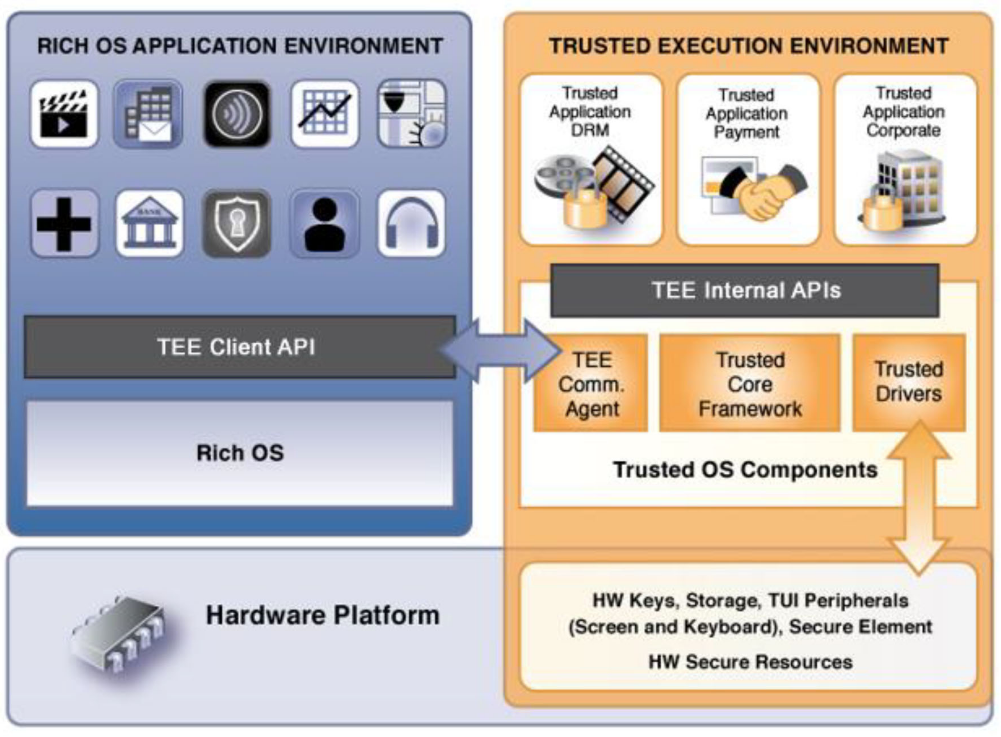
\includegraphics[width=0.5\textwidth]{img/Tee and REE.png}
  \label{fig:tee and ree}
  \caption{Trusted Execution Environment and Rich Execution
  Environment}
\end{figure}

As you can see from figure \ref{fig:tee and ree}, one one device can
run different enviroments at the same time On of those is a
\textbf{Rich Execution Environment} (REE), which is the normal
environment in which one runs any applications or OS. On the other
hand, the TEE is a separate environment isolated from the rest of the
system to run critical tasks and has access to some trusted ankles
like the hwardware keys, the secure storage, peripherals, etc.
TEE can only run on some specific hardware platform made up of trusted
components(not trustworthy, but trusted): the trusted drivers, the
core framework(the execution core) and a set of API accessible only
from trusted applications, the TEE communication agent 

In modern computing, TEE has become an important subject, especially
in the field of "confidential computing," which is actively promoted
by the Confidential Computing Consortium (CCC). The primary goal of
TEE is to protect "data in use," ensuring that nobody else can read or
write the data. Only authorized applications are allowed to process
the data. This approach contrasts with various cryptographic
techniques used to protect "data at rest" and "data in motion."

A key component of TEE, necessary to provide it's services, is the
\textbf{Root of Trust} (RoT), which is an element whose misbehavior
cannot be detected during runtime. The RoT must be \textbf{both
trusted and trustworthy}. It is also part of the Trusted Computing
Base (TCB), which is the set of hardware, firmware, and software
components critical to the system's security. Any vulnerability within
the TCB poses a significant threat to the system’s overall security.

\subsection{TEE Security Principles}

The security principles of a Trusted Execution Environment 
(TEE) involve the following:

\begin{itemize}
    \item Being part of the device's secure boot chain (based on a Root 
    of Trust) and verifying code integrity during each device boot.
    \item Hardware-based isolation from the device’s rich OS 
    environment to execute sensitive code.
    \item Isolation of Trusted Applications (TAs) from each other.
    \item Secure data storage, using a hardware-unique key accessible 
    only by the TEE OS to prevent unauthorized access, modification, 
    and any possibility of data exploitation on other devices.
    \item Privileged and secure access to peripherals (trusted path).
    \item Hardware isolation of peripherals (e.g., fingerprint sensors, 
    displays, touchpads) from the rich OS environment, controlled 
    only by the TEE during specific actions, with no visibility or 
    access by the Rich Execution Environment (REE), including 
    malware.
\end{itemize}

\section{Some TEE Implementations}
\subsection{Intel Identity Protection Technology (Intel IPT)}

Intel Identity Protection Technology (Intel IPT) is a security feature
that operates on a dual-CPU system within Intel processors. This
design leverages the Management Engine (ME), a dedicated CPU that
exists alongside the primary CPU in Intel processors. While the
primary CPU executes user tasks, the ME, integrated into the chipset,
can perform various management and security functions independently.
Typically, the ME is unused in consumer devices, but in corporate
environments, it can be activated even when the device is off via
features like wake-on-LAN, allowing remote management over Wi-Fi or
Ethernet.

Intel IPT uses the ME to run a \textbf{Java applet} isolated from the
main CPU, offering enhanced security for tasks such as cryptographic
key generation and storage, which integrates seamlessly with the
Windows Cryptographic API. Additionally, Intel IPT supports secure
One-Time Password (OTP) generation, as seen in applications like
VASCO's MYDIGIPASS.COM, which use the ME to securely store secrets for
OTPs. Another significant feature is secure PIN entry, where the
chipset manages video output to ensure the security of PIN input by
isolating it from the main system.

The ME's integration into the hardware, running on separate CPU
architecture, exemplifies a physically separated Trusted Execution
Environment (TEE), offering distinct security advantages by isolating
critical operations from the main processing tasks.

\subsection{ARM TrustZone}

ARM TrustZone is a Trusted Execution Environment (TEE) implemented in
certain ARM CPUs, designed to provide a secure and a normal mode
within the same processor. To achieve this, TrustZone extends the
CPU's bus with an additional "33rd bit" that signals whether the
processor is in secure or normal mode. This signal is exposed outside
the CPU, which enables secure peripherals and secure RAM by allowing
the system designer to control access to memory and devices based on
the security mode.

While the TrustZone framework is open and well-documented, it has some
limitations. TrustZone can only support a single secure enclave at a
time, and this security relies on software-based separation between
applications rather than on distinct hardware boundaries, making it
somewhat less secure than fully hardware-isolated environments. ARM is
actively working to expand TrustZone by introducing a third
operational mode to accommodate specific features like attestation.
However, adding this capability presents challenges due to backward
compatibility concerns, as ARM aims to preserve the success of its
platform without disrupting existing applications.

\subsection{Trustonic}

The main issue with TrustZone is that it only one secure enclave. 
To address this issue, Gemalto developed the Trusted Foundations 
system, and Giesecke+Devrient (G+D) created MobiCore. 
Both solutions effectively divide the single secure enclave into 
multiple enclaves by leveraging a smart-card operating system. 
Trustonic’s development is based on MobiCore, requiring 
license fees for implementing the code. Trustonic's TEE OS, 
named "Kinibi," includes enhancements such as version 500, 
which supports 64-bit Symmetric Multiprocessing (SMP) for 
embedded systems. Samsung Knox presents a similar approach 
but additionally incorporates secure boot functionality.

\subsection{Intel SGX}

Intel Software Guard Extensions (SGX) are tightly integrated with the
CPU, providing a hardware-based TEE by modifying memory management to
enhance security. SGX enables the creation of secure enclaves, which
are isolated execution environments protected from access by other
processes, even those with high priority. These enclaves achieve
memory isolation, ensuring that only the code within an enclave can
access its data, providing a high level of hardware-protected
separation.

When an SGX enclave is created, the Intel SGX architecture performs a
measurement, similar to Trusted Platform Module (TPM) practices, by
computing a hash of the executable loaded into the enclave. This
measurement-based security model is essential to SGX’s integrity,
ensuring that only approved code can run within an enclave.

For extended capabilities, SGX can be paired with Intel Identity
Protection Technology (IPT), allowing features such as a trusted
display. However, SGX itself is limited to CPU and memory protection
and does not provide secure input/output channels. When trusted
input-output is required, pairing with Intel IPT enables trusted
interaction with the display.

Intel initially made SGX-1 available across both consumer and
enterprise CPUs, but later revisions—specifically SGX-2—shifted focus
towards server-oriented environments. SGX-2 is now mainly available on
high-end CPUs, such as Intel’s Xeon series, used in data centers.
Furthermore, enclave creation within SGX requires special permissions
and the use of Intel-specific libraries, and all enclave-bound code
must be signed by Intel. This signing requirement means executable
code must be submitted to Intel to receive a signature, which may be a
barrier for some users.

\subsection{Keystone}

Keystone is an open-source framework designed for building Trusted
Execution Environments (TEEs). It allows developers to select only the
necessary features, which helps minimize the Trusted Computing Base
(TCB), because smaller the trust "surface" the better. The
architecture consists of an untrusted environment, such as a
general-purpose operating system, combined with multiple trusted and
segregated enclaves. Keystone is built on top of RISC-V, which offers
customizable open-source hardware options, including
Field-Programmable Gate Arrays (FPGAs) or System-on-Chip (SoC)
designs. The framework incorporates core components along with
cryptographic extensions and supports various execution modes,
including Machine(M), Supervisor(S), and User(U) modes. Additionally, it
features Physical Memory Protection (PMP), which has its
hardware-based access control to different pages of memory. That
avoids that one process can access the memory of another process,
either in general or specifically during a period of time. This helps
to safeguard memory and I/O operations, which are memory mapped.

Usually, TEEs are rigid and un-customizable, with many design
implementation dictated from the underlying hardware, for example
Intel SGX has a large software stack that is not customizable which
means a larger TCB, which is undesirable, AMD SEV
have the same issue and ARM TrustZone has a single TEE. 

The architecture is shown in figure \ref{fig:keystone}. Keystone is
structured to have a \textbf{Security Monition} as the only program
running in Machine mode(the highest privilege mode), which provides
which provides access control between any call coming from the upper
layers towards the hardware. It also provides an \textbf{untrusted
domain} where one can run any OS compatible with the RISC-V 
architecture(even Linux), which will run in Supervisor mode. 
Furthermore, to minimize the TCB, no hypervisor or base operating
systems are required.

On the other hand, one can have many \textbf{Enclaves}, which are 
isolated from the untrusted domain and from each other. Since they
dont need a general purpose OS, they run on a \textbf{Keystone 
Runtime}, which is a small OS that provides the necessary services 
to the specific application. On top of this, the \textbf{Keystone 
Application} runs, which is the actual application that the user 
wants to run.

\begin{figure}[H]
  \centering
  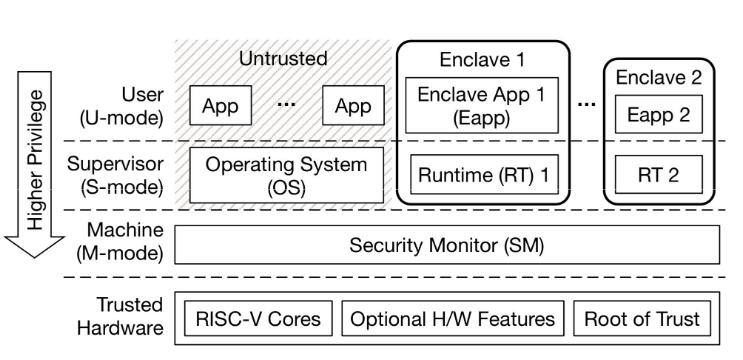
\includegraphics[width=0.6\textwidth]{img/keystone architecture.png}
  \label{fig:keystone}
  \caption{Keystone architecture}
\end{figure}

\begin{boxH}
  For the exam, read the bloody papers.
\end{boxH}

\section{Trusted computing and remote attestation}
Attacker would obviously like to inject malwares at the lowest level
possible, this is to remain undetected while still having access to
the largest part of the system. For this reason the ideal scenario is
to modify the OS is possible, or, alternatively boot an alternative
one under the control of the attacker by modifying the boot sequence
or even the bootloader.

It comes natural after this that the boot system and the OS should be
protected in order to trust the system: for boot sequencing we once
had the BIOS (Basic Input Output System), developed by specific
hardware vendors(no general purpose one available) which was very
difficult to protect, then we had UEFI (Unified Extensible Firmware
Interface) , which is more secure with native support for firmware
signature and verification. After this has been initialized, the OS
can be verified before activation.

So the manufacturer of the platform will sign the firmware, the UEFI,
and the hardware at boot will verify the signature. IF it fails, the
firmware has been tampered with, and the system will not boot. This
step is necessary to guarantee trust in the loaded OS.

\subsection{Rootkits}
This is the generic name for a tool that allows to have root access to
a machine. Of those, there are many kinds.

\paragraph{Firmware Rootkits} Firmware rootkits function by
overwriting the BIOS/UEFI or other hardware firmware. This allows the
rootkit to start running before the operating system even begins to
load.

\paragraph{Bootkits} Bootkits replace the bootloader of the operating
system, ensuring that the bootkit is loaded first when the node is
booted, which occurs before the OS itself initializes.

\paragraph{Kernel Rootkits} Kernel rootkits manipulate a section of
the OS kernel, enabling them to start automatically whenever the
operating system loads, embedding themselves within the core processes
of the OS.

\paragraph{Driver Rootkits} Driver rootkits disguise themselves as
trusted drivers used by the operating system (e.g., Windows) to
interact with hardware. By mimicking a legitimate driver, these
rootkits gain access to hardware resources while avoiding detection.
Don't confuse drivers rootkits with firmware ones, the firmware is
permanently stored in read-only memory, while drivers are part of the
OS and loaded at boot-time.

\section{Root of trust}
In general, protecting software with software can not always be the
best idea, as it may fail or have bugs. For this reason, we need
hardware support to protect the software.
At this end, we have a \textbf{Root of Trust}, which is a hardware 
component that is trusted to behave as expected, and is the foundation
for the chain of trust. The RoT should be always part of the Trusted
Computing Base because hardware is anyway operated by software or
firmware
\subsection{SW root-of-trust}

An example from HP Enterprise illustrates a method for firmware
self-protection, or software root-of-trust. HP Enterprise machines
implements a designated “signature” region at a small fixed location
within the final BIOS image, which is typically 16MB in size. Keep in
mind that this was developed before UEFI.

During manufacturing, the SHA-256 hash of the custom BIOS regions is
calculated. These regions include static code, BIOS version
information, and microcode, but not the hash itself, as its yet to be
initialized, at its only based on components that will never be
updated. The computed hash is then sent to an HPE signing server,
which returns a signed hash image (32 bytes) that includes the
signature and certificate information. This signed hash image is
stored in the BIOS “signature” region.

On power-up, the early BIOS code calculates a hash from the 
specified valid BIOS regions and verifies the validity of the 
stored “signature” contents. If the calculated hash matches 
the stored hash, the boot process proceeds; otherwise, the 
system halts, preventing further booting.

Of course, this method is not perfect, as it is still software-based 
and can be compromised. For example an attacker could replace the 
chip, which is soldered on the board, with a compromised one, or add
another memory chip on the free region of the board, which code will
be executed after the BIOS but before the OS without the integrity 
protection of the signature.

\subsection{HW root-of-trust}
The mechanism just described tries to verify firmware from the
firmware, but can we do better? Yes, we can use a hardware root of 
trust to verify the firmware. 

A hardware root-of-trust for firmware protection typically includes 
self-verification, where a static portion of the firmware authenticates 
the updatable section. This approach allows for an internal method 
of validating firmware integrity directly within the firmware itself. 
Alternatively, firmware verification can be managed by an external 
chip, offering a secure, independent means of affirming firmware 
authenticity.

For example take a look at figure \ref{fig:hw rot}, which shows a x86
Denverton CPU(which is quite old) and implements a 16MB SPI flash
memory, which stores the BIOS. It presents a multiplexer in front of
it that connects to both the CPU and an external cryptographic
microcontroller which can both use the SPI bus and drive the
multiplexer. So the decision of which chip can use the SPI bus is
taken by the external cryptographic microcontroller, which will verify
the integrity of the BIOS before allowing the CPU to boot.

Upon successful validation, this chip allows the x86 CPU to exit its
reset state; otherwise, the CPU remains in reset, ensuring security,
meaning that the chip is the true hardware root-of-trust.

The external chip may also include a fusing option, allowing a public
key hash, which is smaller than the public key, to be securely fused
and later used to verify the signature of the hash stored in the
BIOS's signature region. This validation process is similar to the
internal BIOS self-integrity check, with the added benefit of relying
on an external chip, making it the true hardware root-of-trust.

\begin{figure}[H]
  \centering
  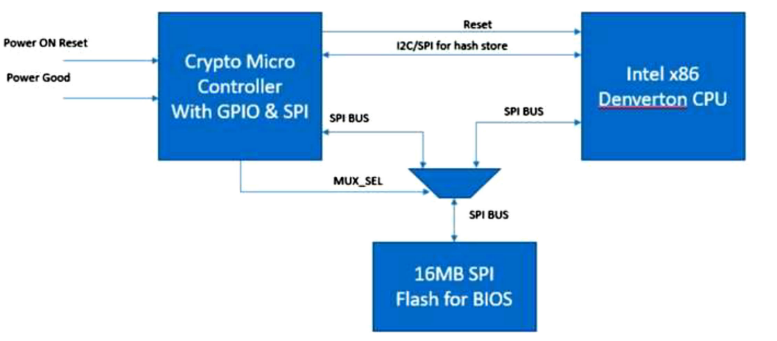
\includegraphics[width=0.6\textwidth]{img/Hw RoT verification.png}
  \label{fig:hw rot}
\end{figure}
\section{Boot Types}
Once we have been able to start the BIOS, the OS can be started.
Different types of boot processes provide varying levels of security
during system startup:

\paragraph{Plain Boot} A plain boot involves no security checks, 
leaving the platform vulnerable to unauthorized modifications.

\paragraph{Secure Boot} In a secure boot process, firmware verifies 
a signature before proceeding. If the verification fails, the platform 
halts, ensuring security from the earliest stages. This process is 
primarily hardware-based and verifies components up to the 
OS-loader.

\paragraph{Trusted Boot} A trusted boot involves the operating system
verifying signatures of critical OS components, such as drivers and
antimalware software. If any verification fails, system operations are
halted. You could have noticed that it assumes that the first part of
the boot up to the firmware was OK and performs verification only of
the operating system components. This type of boot is mainly
software-based and extends verification up to the operational state of
the OS.

\paragraph{Secure boot vs Trusted boot} With secure boot, if the
firmware(BIOS/UEFI/whatever) is compromised, it will not be loaded,
whereas with trusted boot, if the firmware is compromised, the OS
could still be loaded because the firmware is not verified. 


\paragraph{Measured Boot} During a measured boot, the system 
measures each component executed from boot through a defined 
point, denoted as \(X\). Unlike other boot types, measured boot 
does not halt operations if verification fails. Instead, it can securely 
report these measurements to an external verifier, providing 
ongoing insight into system integrity.

What has been just explained is shown in figure \ref{fig:boot types}.
Notice that the trusted drivers and the anti-malware are loaded before
the OS.
% 2 figures 
\begin{figure}[H]
  \centering
  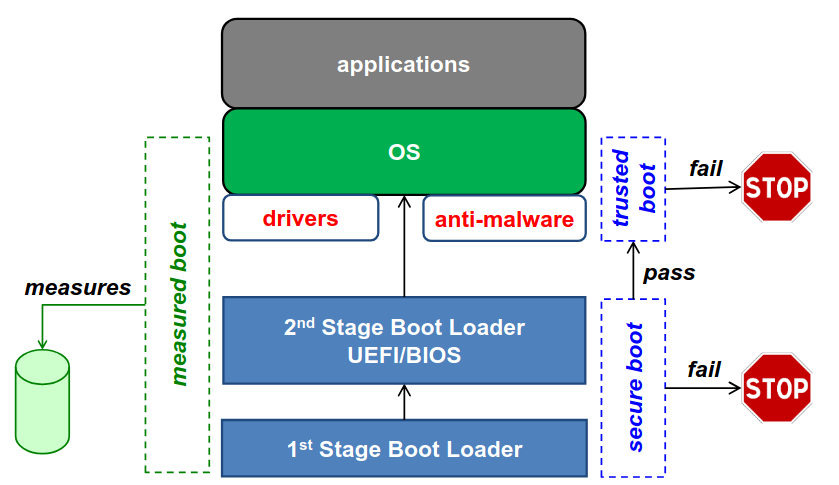
\includegraphics[width=0.6\textwidth]{img/boot types.png}
  \label{fig:boot types}
  \caption{Boot types}
\end{figure}

\subsection*{Windows Boot protection}

Windows 10 and Windows 11 implement a robust boot protection scheme
that combines Secure Boot, Trusted Boot, and Measured Boot to secure
the startup process against malicious interference, as shown in figure
\ref{fig:windows boot protection} . Secure Boot, which is managed by
the hardware manufacturer (e.g., Dell, Lenovo, HP), is the first line
of defense and prevents unauthorized firmware and bootloaders from
running. This step effectively blocks bootkits and ensures that only
trusted firmware initiates the boot sequence.

Following Secure Boot, Windows executes Trusted Boot, which verifies
and loads essential operating system components in a specific order:
first the OS loader, then the kernel, followed by system drivers,
critical system files, and Early Launch Anti-Malware (ELAM) drivers.
ELAM is a fundamental part of anti-malware solutions, as it starts
before any user-space process, offering early protection against
rootkits. The ELAM component must be submitted to Microsoft for
signature to ensure its integrity, enabling a secure foundation for
user-level anti-malware processes to operate later.

In conjunction with Secure Boot and Trusted Boot, Windows also
utilizes Measured Boot, which records each step in the boot process
for verification by an external verifier. If access is granted, this
verifier can query the system to confirm its boot integrity and detect
any potential tampering from the start. This integrated
approach—Secure Boot to lock down firmware, Trusted Boot to load and
verify core OS elements, and Measured Boot to maintain verifiable
logs—creates a strong defense against unauthorized modifications
during the boot process.


\begin{wrapfigure}{r}{0.5\textwidth}
  \centering
  \includegraphics[width=0.5\textwidth]{img/windows boot
  protection.png}
  \label{fig:windows boot protection}
\end{wrapfigure}

\section{Trusted Computing}

Trusted Computing encompasses systems and components designed 
to behave predictably and as expected. In this context, a component 
or platform is considered \textit{trusted} if it consistently performs 
according to predefined expectations, though this does not inherently 
mean it is secure or “good.” Trust in such systems requires verification 
against an expected behavior, rather than an implicit assumption of 
reliability.

A key concept within Trusted Computing is \textit{attestation}, which 
provides verifiable evidence of a platform’s state, allowing assessment 
against a known standard. Another fundamental concept is the 
\textit{Root of Trust}, an inherently trusted component within the 
system that forms the basis for verifying trustworthiness.

Trusted Computing schemes establish trust in a platform by 
identifying its hardware and software components, often through 
a \textit{Trusted Platform Module} (TPM). The TPM plays a crucial 
role in collecting and reporting component identities, offering a way 
to assess hardware and software configurations. This enables 
determination of whether a system’s behavior aligns with expected 
standards, thus supporting the establishment of trust in the platform’s 
integrity.

\subsection{Trusted Computing Base (TCB)}

\begin{boxH}
The Trusted Computing Base (TCB) refers to the \textbf{collection of
system resources}, including both hardware and software, that is
essential in upholding the security policy of a system. 
\end{boxH}

An essential aspect of the TCB is its resilience against compromise;
it must be able to protect itself from threats posed by any hardware
or software outside of the TCB itself.

It is important to note that the TPM \textbf{is not} synonymous with
the TCB of a system. Instead, the TPM serves as a tool for an
independent entity to assess whether the TCB has been compromised. 

In specific implementations, the TPM may also play a preventative
role, ensuring that the system does not start if the TCB fails to
initialize correctly, thus providing an additional layer of security
assurance.

\subsection{Root of Trust (RoT)}

\begin{boxH}
  The RoT refers to a component within a system that must reliably act
  in an expected manner, as any deviation in its behavior cannot be
  detected. 
\end{boxH}

The RoT is essential in establishing trust within a platform
and comprises several foundational components.

The \textbf{Root of Trust for Measurement} (RTM) is responsible for 
taking integrity measurements and transmitting these to the 
\textbf{Root of Trust for Storage} (RTS). Typically, the CPU executes 
the \textbf{Core Root of Trust for Measurement} (CRTM) at boot, 
serving as the first element of BIOS/UEFI code to initiate the 
chain of trust.

The RTS provides a shielded(no one can modify it) and secure storage
environment for critical integrity measurements.
The RTR securely reports the content stored in the RTS, thus enabling
verification of the system's integrity.

\subsection{Chain of Trust}

Our aim is, starting from the lowest level of the firmware, create a
\textbf{chain of trust}.

In a Chain of Trust, each component verifies the integrity of the next
component in sequence. Component A measures Component B and stores
this measurement in the RTS. Then, Component B measures Component C
and similarly stores the measurement in the RTS, continuing this
process down the chain.

Typically, Component A is the CRTM, which is part of the TCB. By using
the \textbf{Root of Trust for Reporting} (RTR), a verifier can
securely retrieve the measurements of Components B and C from the RTS.
For Components B and C to be trusted, Component A must itself be
trustworthy.

\subsection{Trusted Platform Module Overview}

The Trusted Platform Module is an inexpensive component, typically
costing less than 1 dollar, and is available on most servers, laptops,
and PCs. It is designed to be \textbf{tamper-resistant}, although it
is important to note that it is not entirely tamper-proof, meaning
that it is difficult to compromise it, but not impossible.

While the TPM provides security features, it is not a high-speed
cryptographic engine; in fact, it is relatively slow in terms of
processing speed, m.t. doing RSA signatures with it will take forever.
The TPM have to be certified with a \textbf{Common Criteria Evaluation
Assurance Level}(EAL) of 4 or higher, which indicates a certain level
of security assurance, which is quite good indeed.

As a passive component, the TPM requires the CPU to drive its
operations. It does not have the capability to prevent the boot
process; however, it can protect sensitive data and securely report
this information. Consequently, the TPM functions as both the RTS and
the RTR, but it does not serve as the RTM, because we'll perform the
measure and we'll store the results inside the TPM.

The TPM provides secure storage capabilities, functioning as a secure
storage component (RTS) with an extend-only approach. It can report
the content of this secure storage using a digital signature, thus
acting as a reporting entity (RTR). This means that every time that
memory is read outside the TMP, a digital signature computed with a
asymmetric key pair stored inside the TPM is attached to the data.

One of the critical features of the TPM is its hardware random number
generator, which supports various cryptographic algorithms, including
hashing, Message Authentication Code (MAC), and both symmetric and
asymmetric encryption. However, it is important to clarify that the
TPM is not a crypto accelerator, as its performance is relatively
slow.

The TPM also facilitates the secure generation of cryptographic keys
for limited use cases. It supports \textbf{binding}, which encrypts
data using the TPM bind key—a unique RSA key derived from a storage
key. What does that mean? Binding means that if you want to decrypt
this data, you can do that only on the platform that contains that
TPM. Because if you move the data to another platform, they are
encrypted with the key which is not there. This also means that if the
platform broke down, you can't decrypt the data anymore.

Additionally, the TPM allows for \textbf{sealing}, a process
similar to binding, but it also specifies the TPM state required for
the data to be decrypted, or unsealed. This means that the data can be 
decrypted only if the TPM is in a specific state, which is useful to
avoid tampering.

Furthermore, computer programs can utilize a TPM to authenticate
hardware devices. Each TPM chip is manufactured with a unique and
secret \textbf{Endorsement Key} (EK) that is burned in during
production, ensuring that the authenticity of the hardware can be
verified.

\subsection{TPM 1.2}

TPM 1.2 features a fixed set of cryptographic algorithms, which
include SHA-1, RSA, and optionally AES. This version of the TPM
provides a single storage hierarchy specifically for the platform
user, ensuring that key management and storage are centralized.

At the core of TPM 1.2 is a single root key known as the Storage Root
Key (SRK), which is typically an RSA-2048 key. This root key serves as
the foundation for other keys within the TPM, facilitating secure
storage and cryptographic operations.

Additionally, TPM 1.2 incorporates a built-in Endorsement Key (EK)
(RSA-2048) that provides a hardware identity for the platform. This EK
is essential for establishing the authenticity of the TPM and the
device it resides in. 

Another important thing of TPM 1.2 is its capability for sealing
only against the PCRs value, where the measurements are collected. 
\subsection{TPM 1.2}

TPM 1.2 features a fixed set of cryptographic algorithms, which
include SHA-1, RSA, and optionally AES. This version of the TPM
provides a single storage hierarchy specifically for the platform
user, ensuring that key management and storage are centralized.

At the core of TPM 1.2 is a single root key known as the Storage Root
Key (SRK), which is typically an RSA-2048 key. This root key serves as
the foundation for other keys within the TPM, facilitating secure
storage and cryptographic operations.

Additionally, TPM 1.2 incorporates a built-in Endorsement Key (EK)
that provides a hardware identity for the platform. This EK is
essential for establishing the authenticity of the TPM and the device
it resides in. 

Another important feature of TPM 1.2 is its capability for sealing
data to a Platform Configuration Register (PCR) value. This sealing
process ensures that the data can only be decrypted when the platform
is in a specific, verified state, enhancing the security of sensitive
information.
\begin{wrapfigure}{r}{0.5\textwidth}
  \centering
  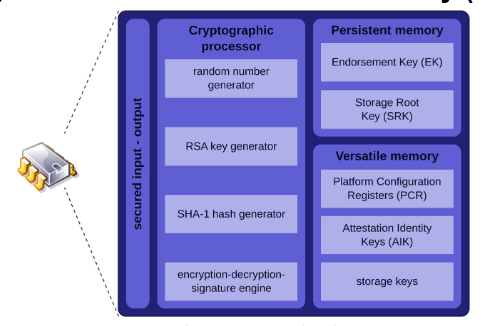
\includegraphics[width=0.5\textwidth]{img/TMP 1-2.png}
  \label{fig:tpm 1.2}
\end{wrapfigure}

\subsection{TPM 2.0}

TPM 2.0 introduces advanced cryptographic flexibility and supports a
range of algorithms, including SHA-1 for backward compatibility,
SHA-256, RSA, ECC-256, HMAC, and AES-128, providing robust options for
secure operations. This version organizes keys into three main
hierarchies: platform, storage, and endorsement. Each hierarchy can
support multiple keys and algorithms, enhancing security management
and allowing for versatile key applications based on specific needs.

A significant feature of TPM 2.0 is policy-based authorization,
enabling more sophisticated and adaptable access controls (in previous
version just one password was required). This policy
framework allows security measures to be tailored according to diverse
requirements and provides a structured way to enforce access
restrictions.

Additionally, TPM 2.0 includes platform-specific specifications
tailored to various application areas, including PC clients, mobile
devices, and automotive environments. Each of these specifications
addresses the unique security requirements of its respective platform,
ensuring that TPM 2.0 can meet the needs of a broad range of use
cases. However, most of the hardware manufacturers implements their
TPMs directly in the CPU or the chipset, meaning that one should check
when buying new hardware: in some cases the TPM is software based on
even virtualized on a dedicated VM thanks to the hypervisor.


\subsubsection{Implementations of TPM 2.0}

TPM 2.0 has several implementation forms, each designed to fit
different hardware and software architectures. The Discrete TPM is a
dedicated chip that implements TPM functionality within its own
tamper-resistant semiconductor package, providing robust security.

In contrast, the Integrated TPM is part of another chip and is not
required to implement tamper resistance. For example, Intel has
integrated TPMs in some of its chipsets, balancing functionality with
space and cost considerations.

The Firmware TPM is a software-only solution that operates within a
CPU's trusted execution environment. Major manufacturers such as AMD,
Intel, and Qualcomm have implemented firmware TPMs, allowing for
flexibility in system design.

Another form is the Hypervisor TPM, which offers a virtual TPM managed
by a hypervisor. This runs in an isolated execution environment and is
comparable to a firmware TPM in terms of security and functionality.

Finally, the Software TPM serves as a software emulator of a TPM,
primarily useful for development purposes. This allows developers to
test and implement TPM functionalities without needing dedicated
hardware.

\subsubsection{TPM 2.0 Three Hierarchies}

TPM 2.0 defines \textbf{three key hierarchies}, each serving distinct
purposes and managing different aspects of security and key storage.

The first hierarchy is the \textbf{Platform Hierarchy}, which is
dedicated to managing the platform’s firmware. This hierarchy utilizes
non-volatile (NV) storage for keys and data, ensuring that critical
firmware-related information is securely maintained.

The second is the \textbf{Endorsement Hierarchy}, which primarily
caters to the privacy administrator. But why we need a privacy admin?
In the early days of the TPM and the Trusted Computing Group (TCG),
there was concern over privacy implications. One issue was that every
time a device’s TPM measured and reported its state, it signed those
measurements with its unique RSA private key. This approach ensured
that the measurements were authentic and uniquely tied to the device,
which was valuable for verifying the integrity of the platform.
However, this method also had a drawback: it revealed the device’s
identity.
If each attestation came from a unique RSA key, it could be traced
back to the same machine each time, compromising privacy.
For this reasons we use different keys for different purposes(key of
the manufacturer, key to identify the owner, \ldots).

Similar to the Platform
Hierarchy, this one also provides storage for keys and data,
emphasizing the importance of privacy in the overall security
architecture.

Lastly, the \textbf{Storage Hierarchy} is designed for the platform’s
owner, who typically also acts as the privacy administrator. This
hierarchy features NV storage for keys and data, allowing for
efficient management of cryptographic assets.

Each of these hierarchies comes with dedicated authorization
mechanisms, such as passwords, and specific policies to govern access
and usage. Additionally, each hierarchy utilizes a unique seed for
generating the primary keys, further enhancing the security and
integrity of the TPM's operations.

\subsection{Using a TPM for Securely Storing Data}

Utilizing a TPM for securely storing data
involves several key considerations to ensure both security and
accessibility.

One primary advantage of using a TPM is its physical isolation. The
storage occurs within the TPM itself, specifically in NVRAM, which
helps safeguard sensitive information. This storage is very small, so
ut usually stores primary keys and permanent keys

To enhance security, Mandatory Access Control (MAC) mechanisms are
employed, which govern how data and keys are accessed within the TPM.
This cryptographic isolation ensures that even if data is stored
outside the TPM, such as on a platform's hard drive, it remains
protected.

When storing keys or data outside the TPM, it is crucial that the
information is encapsulated in a secure format, often referred to as a
blob. This blob must be protected, typically by encrypting it with a
key controlled by the TPM. The use of MAC further reinforces the
security measures, ensuring that access to the stored data is tightly
regulated.

\subsection{TPM Objects}

TPMs utilize various objects to manage cryptographic keys and secure
data. One of the primary types of objects within a TPM is the
\textbf{primary keys}, which includes endorsement keys and storage
keys. These keys are derived from one of the primary seeds stored
within the TPM. Notably, the TPM does not return the private value of
these keys; instead, they can be re-created using the same parameters,
assuming that the primary seed remains unchanged.

In addition to primary keys, TPMs also handle keys and sealed data
objects (SDOs). These objects are protected by a Storage Parent Key
(SPK), which is necessary within the TPM to load or create a key or
SDO. The randomness required for key generation and other
cryptographic functions is provided by the TPM's built-in Random
Number Generator (RNG). 

When a key is generated, the TPM returns the private part, which is
protected by the SPK. However, it is essential to note that this
private part must be stored securely, as its integrity is critical to
maintaining the overall security provided by the TPM.

\subsection{TPM Object Areas}

Trusted Platform Modules (TPMs) categorize the storage structure of
objects into distinct areas, each serving a specific purpose:

\begin{itemize}
  \item \textbf{Public Area:} This area is utilized to uniquely
    identify an object, providing essential information for the
    management of keys and data.

  \item \textbf{Private Area:} Containing the object's secrets, this
    area exists solely within the TPM. It is crucial for maintaining
    the confidentiality and integrity of the keys and data stored
    within the module.

  \item \textbf{Sensitive Area:} This consists of the encrypted
    private area, specifically designed for use when storing sensitive
    data outside of the TPM. It ensures that even when data is not
    housed within the TPM, it remains secure through encryption.
\end{itemize}

\subsection{TPM Platform Configuration Register (PCR)}

The Platform Configuration Register (PCR) serves as the TPM
implementation of Root of Trust for Storage (RTS) and is a core
mechanism for recording platform integrity. PCRs maintain their values
and can only be reset during a platform reset or through a hardware
signal, which ensures that any malicious code cannot manipulate or
retract its measurements.

PCRs are extended using a cumulative hash, following the formula:

\[
\text{PCR}_{\text{new}} = \text{hash}(\text{PCR}_{\text{old}} \, || \, \text{digest\_of\_new\_data})
\]
Basically, the new PCR value is the hash of the old PCR value and the 
new data. This process is repeated for each new piece of data that
needs to be added to the PCR.

This process is commonly referred to as the EXTEND operation (keep in
mind that it's not commutative).
Additionally, PCRs can be utilized to gate access to other TPM
objects. For example, BitLocker uses PCR values to seal disk
encryption keys, ensuring that the keys can only be accessed when the
platform is in a known and trusted state.

\subsection{Measured Boot}

Measured boot builds on secure and trusted boot principles by using
TPM functionality to verify system integrity throughout the boot
process. The key here is that a TPM is available—whether as a separate
chip or firmware module—enabling attestation at each step.

The process begins with the Core Root of Trust for Measurement (CRTM)
located in the boot ROM’s first-stage bootloader. This trusted
component takes the first measurement by capturing the state of the
next component in line, the second-stage bootloader, and stores this
in the TPM’s Platform Configuration Registers (PCRs). This baseline
measurement is critical, as it establishes initial trustworthiness for
everything that comes afterward.

Once the second-stage bootloader is loaded, it continues the process
by measuring the operating system, which can also measure subsequent
applications if needed. The idea is simple: measure each part of the
boot sequence and store these measurements in the PCRs, creating a
chain of trust from the very start.

The accumulated values in the PCRs provide a snapshot of the system’s
integrity, which an external verifier can check to confirm everything
is as expected. Though an internal verifier is possible, an external
one is often more reliable in case an attacker has compromised the
internal components. This setup allows measured boot to act as a
strong line of defense, verifying each stage and ensuring a trusted
environment.

\begin{figure}[H]
  \centering
  \includegraphics[width=0.6\textwidth]{img/Measured boot.png}
  \caption{Measured boot}
\end{figure}
\subsection{Remote attestation procedure}

Remote attestation leverages the values stored in the TPM’s PCRs
during the measured boot process, enabling an external verifier to
confirm the system's integrity. Here’s how it works:

First, an external verifier, which could be a trusted system on the
network, sends a unique challenge (often a nonce) to the device
holding the TPM. This challenge prevents replay attacks by ensuring
that each attestation session is fresh and unpredictable. The platform
then gathers the values of the PCRs requested by the verifier and
packages them along with the challenge.

This package of data—containing the PCR values and the response to the
nonce—is signed using a key unique to the device. This signed response
assures the verifier that it’s seeing legitimate measurements tied to
that specific device.

When the verifier receives the signed package, it performs several
checks:
\begin{enumerate}
  \item \textbf{Signature Validation}: It verifies the signature to
    ensure the data hasn’t been tampered with and is genuinely from the
    device.
  \item \textbf{Identity Validation}: It checks that the device’s
    identity matches expected values, using a stored list of authorized
    machines to confirm that the device is part of the network.
  \item \textbf{Measurement Validation}: Finally, the verifier compares
    the PCR values against known "golden values" stored in a database.
    These golden values reflect the expected configurations for each
    device type—taking into account variations in hardware, firmware,
    and software.
\end{enumerate}

If the PCR values match the golden values, the verifier can
confidently conclude that the system is in a known and trusted state.
If there’s a mismatch, an alert is raised, signaling that the device
may have been compromised or misconfigured.

This remote attestation process provides a robust way to ensure system
integrity across a network by verifying both the software status and
identity of each device, making it a valuable tool for network
security.

\begin{figure}[H]
  \centering
  \includegraphics[width=0.6\textwidth]{img/remote attestation
  procedure.png}
  \caption{Remote attestation procedure}
\end{figure}

\subsection{Management of Remote Attestation}

Remote attestation has been performed, and it has failed. What now?
Management of remote attestation is most important when the
attestation process fails. 

One critical aspect is whether to implement only boot attestation,
which is static, or to include periodic (dynamic) attestation as well.
This decision should take into account the attack model, especially
with respect to runtime vulnerabilities that could be exploited.

The \textbf{periodicity of the attestation} operation is another
important consideration, as it must align with the speed of potential
attacks. A cycle of operations which include the time
required for signature verification, protocol execution, and database
lookups, are typically in the range of several seconds due to the
inherent slowness of TPMs, and for some cases is acceptable, but for
others a window of exposure of even 5 seconds is excessive. 
And that is a limit, not of the attestation, but of the physical
implementation.

Another challenge in remote attestation management is
\textbf{whitelist generation}. This process can be complex in general
but may be less difficult in limited environments, such as Internet of
Things (IoT) devices, edge devices, Software-Defined Networking (SDN),
and Network Function Virtualization (NFV). 

Furthermore, it is essential to label components appropriately—such as
good, old, buggy, or vulnerable—and to include configurations from
sources like Management and Orchestration (MANO) or network management
tools. While generating labels can be straightforward if the data is
file-based, it becomes significantly more challenging when dealing
with memory-based data.
\subsection{TCG PC Client PCR use (architecture)}
According to the Trusted Computing Group for a PC client the PCRs are
used for various purposes:
\begin{wrapfigure}{r}{0.5\textwidth}
  \centering
  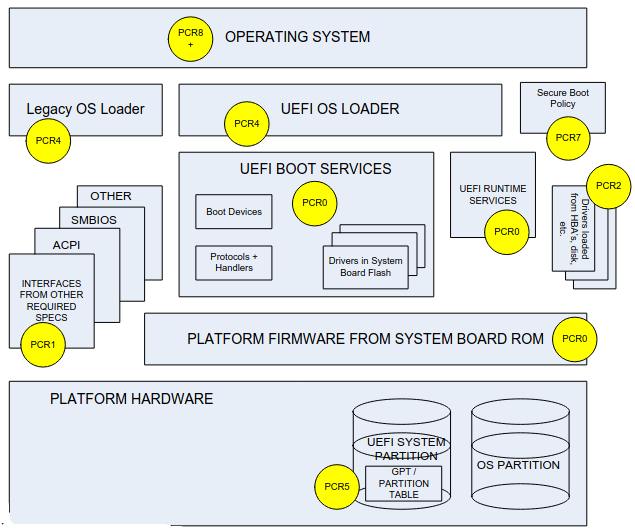
\includegraphics[width=0.5\textwidth]{img/TCG PC Client.png}
  \label{fig:TCG PC Client PCR use}
  \caption{TCG PC Client PCR architecture}
\end{wrapfigure}

\begin{itemize}

  \item PCR0 is measuring the Platform firmware from system board ROM
    and it is a fixed value given one version of the firmware.
    Typically, in a database there are different values for PCR0
    according to the version of the firmware and the version running
    in a device could be deduced by these values. It also stores the
    UEFI boot services, UEFI runtime services.
  \item PCR1 contains the hash of various extensions of the firmware
    (ACPI, SMBIOS, OTHER).
  \item PCR2 drivers loaded from the disk.
  \item PCR3 is not here. That means it's not used for PC.
  \item PCR4 is the part of the UEFI OS loader and of the Legacy OS
    Loader
  \item PCR5 is for the Platform hardware, for example it is reading
    and computing the hash of the partition table. That is important
    if someone manipulated the hardware.
  \item PCR7 contains the Policy for Secure Boot.
  \item All registers from PCR8 to above are given to the OS to decide
    what will be used for.
\end{itemize}
For all the registers up to PCR7 the values can be predicted. They
will depend on the kind of platform, version of the firmware or
driver. These values are in the golden: if there are wrong values in
those registers the system cannot be trusted.
\begin{table}[H]
  \centering
  \begin{tabular}{|p{0.1\textwidth}|p{0.9\textwidth}|}
    \hline
    \textbf{PCR Index} & \textbf{PCR Usage} \\ \hline
    0 & SRTM, BIOS, Host Platform Extensions, Embedded Option ROMs and
    PI Drivers \\ \hline
    1 & Host Platform Configuration \\ \hline
    2 & UEFI driver and application Code \\ \hline
    3 & UEFI driver and application Configuration and Data \\ \hline
    4 & UEFI Boot Manager Code (usually the MBR) and Boot Attempts \\
    \hline
    5 & Boot Manager Code Configuration and Data (for use by the Boot
    Manager Code) and GPT/Partition Table \\ \hline
    6 & Host Platform Manufacturer Specific \\ \hline
    7 & Secure Boot Policy \\ \hline
    8-15 & Defined for use by the Static OS \\ \hline
    16 & Debug \\ \hline
    23 & Application Support \\ \hline
  \end{tabular}
  \caption{PCR Index and Usage}
  \label{table:pcr_usage}
\end{table}

\subsection{Measured Execution}
Previously, we discussed measured boot, which verifies the integrity 
of the system during the boot process. We would like to extend this
functionality to the application that runs on the OS, but to do so we
would have to store the measurements in PCRs, which are limited in 
number.For this reason we can simply use one PCR and extend the
measurements of each application.

Another issue also arises: the value of the PCR depends on the
execution order, in fact starting an application A before an
application B will result in a different value of the PCR than
starting the application B before the application A.
For this reason, the OS can measure the application before loading it
and perform the extend operation of the PCR, but not all OS are able
to do so(the superior OS can).
\subsubsection{Linux’s IMA}

The \textbf{Integrity Measurement Architecture} (IMA) in Linux is a
standard component of the Linux kernel(one needs to enable it)
that extends attestation capabilities to dynamically executed
elements, such as applications. It provides mechanisms for collecting,
storing, appraising, and protecting measurements to ensure the
integrity of files accessed on the system.
It can perform various operations:

\begin{itemize}
  \item \textbf{Collection}: IMA measures a file before it is
    accessed, creating an integrity measurement to track any potential
    alterations.
  \item \textbf{Store}: The measured data is added to a
    kernel-resident list, known as the Measurement List (ML), and the
    IMA PCR (specifically PCR 10) is extended to reflect these
    measurements, making them available for attestation purposes.
  \item \textbf{Appraise} (optional): IMA can enforce local validation
    of a file's measurement by comparing it to a "good" value stored in
    the file's extended attributes. This step helps to ensure that the
    file remains in a trusted state, but is a feature which
    is not required for measured operations
  \item \textbf{Protect} (optional): IMA can secure a file's extended
    security attributes, including the appraisal hash, against offline
    attacks. This prevents unauthorized modifications to these
    attributes when the system is not active.
\end{itemize}
The appraise feature is most interesting: lest's suppose that one
think that, for example, a python executable has been compromised. One
can use an extended attribute to store the hash of the python 
executable and compare it with the hash of the python executable 
measured by the IMA. This happends before it's been executed,
automatically by the OS. If the hashes are different, the python
executable is not executed.

When the IMA starts, it extends UEFI's measured boot concept to the OS
and applications by using PCR 10. It begins by storing a "boot
aggregate," which is a hash of all PCR values from 0 to 7—these PCRs
capture UEFI-related measurements. This boot aggregate establishes a
continuity between the boot measurements and IMA's ongoing monitoring,
preventing certain types of attacks.

IMA is configurable through an "IMA template," which defines what gets
measured. A common template, "IMA-NG," is often used, but the template
can be customized to fit specific needs. IMA then logs these
measurements in the kernel security filesystem, where they’re stored
as ASCII runtime measurements, allowing access to a detailed record of
measured files and executables. For example, each entry includes the
PCR 10 value, a template hash, and hashes for each file, showing the
order in which each executable or library was measured.

\begin{table}[h!]
  \centering
  \begin{tabular}{|c|c|c|c|c|}
    \hline
    \textbf{PCR} & \textbf{template-hash} & \textbf{template} & \textbf{filedata-hash} & \textbf{filename-hint} \\
    \hline
    10 & 91f34b5[...]ab1e127 & ima-ng & sha1:1801e1b[...]4eaf6b3 & boot\_aggregate \\
    10 & 8f16832[...]e86486a & ima-ng & sha256:efdd249[...]b689954 & /init \\
    10 & ed893b1[...]e71e4af & ima-ng & sha256:1fd312a[...]6a6a524 & /usr/lib64/ld-2.16.so \\
    10 & 9051e8e[...]4ca432b & ima-ng & sha256:3d35533[...]efd84b8 & /etc/ld.so.cache \\
    \hline
  \end{tabular}
  \caption{Example of IMA Measurement List}
\end{table}


To verify these measurements, a verifier can request the current PCR
10 value. The machine responds with this value along with the detailed
measurement list. To validate, the verifier starts with a zero value,
incorporates the boot aggregate by combining PCRs 0 through 7, and
then processes each measurement in the order they were originally
extended into PCR 10. This step-by-step verification ensures that the
system's state aligns with expected integrity values.

\begin{listing}
  \centering
  \begin{verbatim}
myPCR10 = 0
myPCR10 = extend(boot_aggregate)

foreach measure M of component C
    if (C not authorized) then raise alarm
    if (M != gold_measure(C)) then raise alarm
    myPCR10 = extend(M)
end foreach

if (myPCR10 == PCR10) OK else raise alarm
  \end{verbatim}
  \caption{IMA verification}
\end{listing}



\chapter{Social Engineering}
First of all, we should dead with what sociology really is, then we
will master the vocabulary to be able to put a name on phenomenons,
and then we will deal with social engineering. We will apply some
sociological theories to think of a new way to perceive and represent
the complex relationships among machines and human beings.
\section{Sociology}
Let's kick off with a definition of sociology.

\begin{boxH}
  Sociology is the \textbf{science of social phenomena} subject to
  natural and invariable laws, with the goal of discovering these
  laws.

  - Auguste Comte, 1839
\end{boxH}
The important point is not the definition, but the fact the definition
contains many information about the cultural environment from which it
comes. If you think about it, the definition focuses on the scientific
method, which tries to quantify something in a deterministic fashion,
becase one believe that all the necessary informations are already
there. But natural laws are more complicated than these and human laws
are even more complicated. 

To sum this up, first, one can quantify social interactions, today we
do apply maths and statistics to social facts. Second there's a sort
of cause and effect relationship between social phenomena: just as at
that time they believed that nature was describable in this way, they
came up with the idea that society could be as well.

Another definition of sociology is the following:
\begin{boxH}
  Sociology is the study of human social life, groups, and societies.
  - Antony Giddens
\end{boxH}
As you can see, the scope of the definition was quite reduced.

There are also other figures that are important to keep in mind. The
first one is German sociologist and economist Max Weber, because he
guides us in understanding two key aspects of sociological inquiry.
First, it is \textbf{evolutive}: We live in a context of digital and
analogical interactions in which, if you don't take a stand for
something or for somebody, it means you're out of the debate. If you
think about it, social media algorithms have been coded in order to
emphasise this sort of polarisation effect, because the more polarised
the debate, the more engaged the debate becomes, which makes sense for
an economical standpoint, and this kind of interaction is becoming the
natural of the way we interact. The second lesson is that the
\textbf{uncertainty of data} is the only certainty we have. There
might be systemic errors in your data sets, accidental errors, and
they are due to the sometimes the impossibility to have direct access
to some sort of phenomenon (think for instance about criminality). The
fact that they are somehow at least partly accessible limits the scope
of the conclusions you are reaching. Even biases and subjectivity are
a problem, for instance, one reinvents the past when one tries to 
recall it, which is just the way our brain works.

The second relevant figure is Charles Wright Mills, a sociologist from
the US, the 50s and the 60s, the one who studied the white collars.
The key concept is the \textbf{sociological imagination}, which is the
ability to see when you want to social phenomena through the eyes of
scientific inquiry, not through common sense and stereotypes.



\subsection{Basic Sociological Vocabulary}

Sociology uses specific terms to describe the elements of society and
social behavior. Below are key concepts:

\textbf{Norms} are the rules and expectations by which a society
guides the behavior of its members. With members we refer to social
actors, which can be individuals, groups, or institutions. After all,
sociology uses theatrical metaphors to describe the interactions
within a society. So, norms are sets of rules that you are given
because you are recognised as a member, as an actor within a context,
a society. There are mainly two types of rules. Explicit norms and
implicit, or tacit, norms. Cyber criminals rely mostly on the latter 
ones, because they can be broken more easily. After all, they are
invisible to newcomers, and they are not written down, and they have
to be learned by experience.

\textbf{Values} refer to collective ideas about what is good,
desirable, and proper. Those are tricky elements, because the more
social they are, the less they seem to be, because, if a set of values
is very well spread within a group, each member of the group feels
like the values are obvious.

\textbf{Role} encompasses the set of norms, behaviors, and
expectations associated with a particular social status or position
within society. Roles guide how individuals are supposed to act and
interact with others in specific contexts. As described before, they
are strictly connected with the idea of playing the game or acting
society. We are usually more than a role, but we decide to show only 
a part of ourselves according to the context we are in. Roles are not
self-assigned, they are recognised by the others, and indeed,
sometimes when you feel you are not recognized in one role, you feel
uncomfortable.

\textbf{Social Structure} is the organized pattern of social
relationships and social institutions that together constitute
society.

\textbf{Culture} consists of shared beliefs, values, and practices. In
the end, humankind was able to organize social interactions against
chaos. That's why we can speak of societies, no matter how simple,
small or very complex and big they are. But they are very well
structured.

\subsection{The social iceberg}
To conclude this sociological journey, consider the image of an
iceberg—a fitting metaphor for social relations. Above the surface, we
find two dimensions. The first relates to corporality: our body,
nervous system, and senses help us perceive and interact with the
world. However, our senses are not foolproof; they can mislead us.
Hallucinations and memory distortions, for instance, demonstrate the
limits of our perception. Witness accounts of even simple events, like
a car accident, often differ significantly from each other and from
camera footage. This highlights how imperfect and subjective our
senses are—they are both gateways to the environment and sources of
error.

The second dimension involves processing sensory input through our
mental filters: past experiences, memories, learning, and
adaptability. These filters shape how we interpret the world and
decide how to act—or not to act. Sociologically, both action and
inaction are forms of behavior, influenced by this interplay of
perception and processing.

Below the surface of the iceberg lies a deeper realm of human
experience. This includes the mental "autopilot" we rely on to
navigate most of our daily activities. We don't constantly
"meta-think" or reflect on every action, like sitting in a chair or
walking. These routines are built on assumptions that rarely fail
us—until they do. When something disrupts our expectations, it forces
us to pause, question, and adjust. This reflects the philosopher
Hume's insight: we assume the sun will rise tomorrow because it always
has, but that certainty is not guaranteed.

Additionally, from birth, we begin absorbing knowledge through a
process sociologists call primary socialization. Caregivers teach
us how to express needs, interact with others, and adapt to our
environment. Early lessons—both instinctive and taught—form the
foundation of our behavior.

As we grow, secondary socialization takes over, enriching our
"autopilot" with experiences from school, friendships, work, and
culture. These interactions shape our social network, values, and
identity. From the music we enjoy to the relationships we build, this
ongoing process continually informs how we navigate and understand the
world.

\begin{figure}[H]
  \centering
  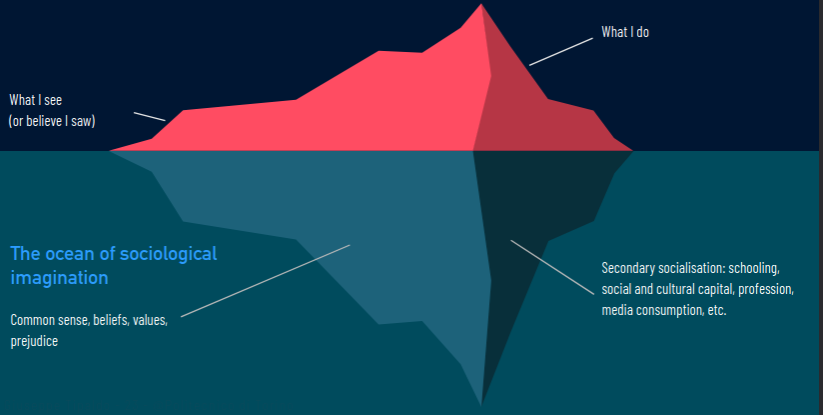
\includegraphics[width=0.5\textwidth]{img/sociology iceberg.png}
\end{figure}

\section{Vocabulary}
In general it is important to provide a clear definition of complex
phenomena to be able to apply more then a label to them. As such, we
will try to analyze different attempts to give a name to cyber
criminal activities. During the years, many definitions have been
provided, meaning that we need a way to classify them too.

\begin{boxH}
  One of the leading factors leading to difficulties in estimating
  cybercrime is exactly the fact that we don't have very well formed
  definitions nor a rigorous classification method.
\end{boxH}

The wider and richer the vocabulary, the more complex the thoughts you
can make, you can formulate.

We begin with the period from 1995 to 2000, during which the term
"cybercrime" was not even the dominant word used in discussions
related to the field. This stands in stark contrast to the following
window, 2001 to 2018, when "cybercrime" emerged as the most frequently
used term in scientific literature. It’s worth noting that 30 years
ago, there wasn’t even a widely agreed-upon term to describe
cybercrime in a scientific context. 

While 30 years might seem like a long time, it’s relatively brief in
the grand scheme of scientific progress. At the same time, it
represents a significant period during which research and terminology
have evolved. For instance, efforts to classify the various forms of
cybercrime often result in taxonomies that, no matter how
comprehensive, fall short of fully bridging the gap between
theoretical frameworks and real-world occurrences.

From such classifications, it becomes evident that creating broader
categories or groups can be helpful. These allow for more efficient
communication and problem-solving without the need to enumerate every
specific instance when referring to a broader class or subclass of
cybercrime.

\begin{figure}[H]
  \centering
  \includegraphics[width=0.7\textwidth]{img/cybercrime
  definitions.png}
  \caption{Organizational definitions of cybercrime.}
\end{figure}

As you can see, the definitions are quite different from each other,
some are broader, some are more specific.

There are several attempts to try and make it more clear and try to
classify those definitions in order to make it simpler to understand
for those maybe who lack some tech knowledge about cybersecurity. For
example, one proposal is to adopt a sort of categorical approach to
the systematization of definitions. A categorical approach is a 
systematic way to classify things, and with this approach we can
discern between cyber-enabled crimes and cyber-dependent crimes. 
\textbf{Cyber-enabled} crimes are traditional crimes that predate the
advent of the technology, and are now facilitated or have been made
easier (i.e., enabled) by cyber technology. Crimes range from
white-collar crime to drug trafficking, to online harassment,
terrorism and beyond.

\textbf{Cyber-dependent crimes} are crimes that arose with the advent
of technology and cannot exist (i.e., dependent) outside of the
digital world, e.g., hacking, such as ransomware attacks or
hacktivism.

This classification is very rigid, in fact, if you belong to one of
those category, you can't belong to the other one. We can try to fix
this rigidity with another approach: if we consider the two
classifications as the extremes of a continuous function, each criminal
activity should be placed somewhere on this continuum.

\begin{figure}[H]
  \centering
  \includegraphics[width=0.8\textwidth]{img/continuum
  classification.png}
\end{figure}

A less rigid categorical approach is possible without resorting to
the continuum, by discerning different properties of a crime and
activities. 


From figure \ref{fig:trichotomic-def}, we can see 2 different
classification, which provides different labels for the same
definitions. This is just to say that even today, we don't have a
clear classification.

\begin{figure}[h]
  \centering
  \includegraphics[width=0.8\textwidth]{img/trichotomic
  definition.png}
  \caption{Trichotomic definition of cybercrime.}
  \label{fig:trichotomic-def}
\end{figure}

As for what concerns the definition of what a cybercrime is, there's
no a clear definition. Those can vary depending on perspective,
sensitivity, and the traits emphasized in its definition. Different
stakeholders, institutions, and interests shape how it is understood
and defined. What one might highlight as key traits or concerns may
not align with another's perspective, and all those factor may
influence the definition of cybercrime.

Mr. Frederick Chung, a former research director at the NSA, describes
cybersecurity as fundamentally rooted in \textbf{adversarial social
interactions}. While it clearly involves technology and
engineering—emphasized by the "cyber" prefix—what sets it apart is its
focus on the science of society and the dynamics of conflict.
Essentially, cybersecurity deals with humans defending systems and
machines against other humans, which often use machines as tools for
attack. This definition highlights the need for a multidisciplinary
approach that goes beyond traditional technical disciplines to fully
grasp the complexities of cybersecurity.

Fom this definition, we can expand a bit more on the contect of
\textit{cyber}, which is usually a prefix that refers to the
\textbf{cyberspace}, a term coined by William Gibson in his 1984 novel 
\textit{Neuromancer}. This same term is used by Public Safety Canada 
to define "he electronic world created by interconnected networks of
information technology and the information on those networks".
The enphasis in this definition is on two things: the communication
that is mediated by the network, that isn't necessarily between
humans, but may be between machines, and the \textbf{information} that
is conveyed by the network, and also the stimulus for interconnection.

\subsection{Cybersecurity and it's many definitions}

The discourse on security revolves around mitigating risks and
controlling hazards, often represented by attackers—whether human or
machine—targeting us or our properties. Security involves protecting
these properties and addressing potential dangers that could harm
them. An essential dimension of this discussion is the ability to ask
the right questions, as highlighted by Buzz, Weaver, and Wild (1998).
They propose a cognitive framework for analyzing security in
cyberspace: understanding who is securing what, against which threats,
for whom, and why, along with the conditions and outcomes. This serves
as a conceptual checklist for planning or analyzing security
strategies.

According to Craigen et al(2014), we may identify 9 different
deinitions about cybersecurity.

\begin{enumerate}
  \item “Cybersecurity consists largely of defensive methods used to
    detect and thwart would-be intruders.” (Kemmerer, 2003)
  \item “Cybersecurity entails the safeguarding of computer networks and
    the information they contain from penetration and from malicious
    damage or disruption.” (Lewis, 2006)
  \item “Cybersecurity is the collection of tools, policies, security
    concepts, security safeguards, guidelines, risk management
    approaches, actions, training, best practices, assurance and
    technologies that can be used to protect the cyber environment and
    organization and user's assets.” (ITU, 2009)
  \item “The ability to protect or defend the use of cyberspace from
    cyber-attacks.” (CNSS, 2010)
  \item “The state of being protected against the criminal or
    unauthorized use of electronic data, or the measures taken to
    achieve this.” (Oxford University Press, 2014)
  \item “The activity or process, ability or capability, or state
    whereby information and communications systems and the information
    contained therein are protected from and/or defended against damage,
    unauthorized use or modification, or exploitation.” (DHS, 2014)
  \item “The art of ensuring the existence and continuity of the
    information society of a nation, guaranteeing and protecting, in
    Cyberspace, its information, assets and critical infrastructure.”
    (Canongia \& Mandarino, 2014)
  \item “The body of technologies, processes, practices and response and
    mitigation measures designed to protect networks, computers,
    programs and data from attack, damage or unauthorized access so as
    to ensure confidentiality, integrity and availability.” (Public
    Safety Canada, 2014) 
  \item “Cyber Security involves reducing the risk of malicious attack
    to software, computers and networks. This includes tools used to
    detect break-ins, stop viruses, block malicious access, enforce
    authentication, enable encrypted communications, and on and on.”
    (Amoroso, 2006)
\end{enumerate}

Let's now talk a little bit about those definitions.

Cybersecurity is a big, complex topic, and different people think
about it in different ways. Over time, researchers and experts have
developed various approaches—or paradigms to help us understand and
deal with cybersecurity challenges. Let’s take a closer look at a few
of these paradigms.

The first and most common is the \textbf{defense paradigm}. This
approach is all about protecting systems as much as possible. It’s
focused on avoiding attacks, preventing harm, and keeping everything
safe. The idea is straightforward: keep the bad stuff out and protect
what matters. It’s an idealistic view, assuming that if you work hard
enough, you can secure systems completely. While this is great in
theory, reality often throws curveballs.

That’s where the \textbf{continuity paradigm} comes in. It’s a more
practical take, accepting that perfect protection isn’t always
possible. Instead of aiming for total safety, this approach focuses on
surviving attacks and minimizing damage. Think of it like disaster
management—when something goes wrong, you figure out what’s most
important to save and focus your energy there. Sure, you might lose
some things, but the goal is to avoid a complete collapse. It’s about
keeping the core functions alive, even if other parts take a hit.

Next up is the \textbf{ecological paradigm}, which takes a broader view.
This one treats cybersecurity like an ecosystem, where everything is
interconnected and balanced. A system works best when all its parts are
in harmony, and disruptions to one part can ripple through the rest.
This perspective reminds us that systems are complex, and it’s not just
about protecting individual pieces—it’s about keeping the whole thing
working smoothly. Balance is key, and when things get out of whack,
mitigation strategies help bring them back on track.

Finally, there’s the \textbf{risk paradigm}. This approach gets
straight to the numbers. It’s all about assessing risks, measuring how
likely something bad is to happen, and figuring out the potential
impact. Once you know the risks, you can weigh the costs of protection
against the potential losses. Sometimes, it might even make more sense
to accept the risk rather than spend too much on safeguarding something
that isn’t worth it. This paradigm is especially useful when resources
are limited, and you need to make smart decisions.

These paradigms don’t compete with each other—they work together. The
\emph{defense paradigm} sets the ideal goal, the \emph{continuity
paradigm} helps when things don’t go perfectly, the \emph{ecological
paradigm} looks at the bigger picture, and the \emph{risk paradigm}
makes sure decisions are grounded in reality.

Together, they show just how diverse and dynamic cybersecurity is.
There’s no one-size-fits-all solution, but by combining these
perspectives, we can handle the challenges and keep adapting to new
threats.

Now, do we need a 10th definition? According to the professor, yes we
do. But to do so, we have to consider the similarities and differences 
between the definitions we have already seen. 
As for what concerns the similarities, they all seems to revolve
around a few core ideas:
\begin{itemize}
    \item \textbf{Technology}: At its core, cybersecurity depends on
      technology. Cyberspace itself wouldn’t exist without it.
    \item \textbf{Events}: Cybersecurity focuses on events—incidents
      that need analyzing, mitigating, or learning from. Cybercrimes
      often aim to stay hidden, making evidence critical.
    \item \textbf{Methods and Strategies}: It’s not just about
      reacting to threats but having processes and plans to protect
      systems.
    \item \textbf{Human Involvement}: Despite advancements in AI and
      automation, human input remains essential for oversight and
      adaptation.
    \item \textbf{Evolving Focus}: Over time, cybersecurity has
      shifted its focus—from protecting machines to data, privacy, and
      beyond. Legal definitions of cybercrimes have evolved too.
\end{itemize}


But there are also some distinguishing factors that set the 
definitions apart:
\begin{itemize}
    \item \textbf{Sociotechnical Perspective}: Cybersecurity requires
      both technical skills and insights from social sciences and
      humanities. It’s about understanding human and human-machine
      interactions, as highlighted by the need for a multidisciplinary
      approach.
    \item \textbf{Scaling the Problem}: Some definitions address
      cybersecurity on a broader scale, emphasizing its role in
      national security. This includes diplomacy, financial systems,
      espionage, and other political and economic concerns.
    \item \textbf{Warfare and Resilience}: Cyberattacks are now
      integral to modern warfare, affecting conflicts worldwide.
      Resilience, adaptability, and building systems that remain
      connected and reliable under attack are crucial.
\end{itemize}

Now, let's have our 10th definition:
\begin{boxH}
  Cybersecurity is the organization and collection of resources,
  processes, and structures used to protect cyberspace and
  cyberspace-enabled systems from occurrences that misalign \textit{de
  jure} from de facto property rights.
\end{boxH}

\begin{boxH}
  Disclamer: at this point, the professor just followed his stream of
  consciousness for 1 hour and i half, and even after reading it all,
  i still don't know what he was talking about. It was just like a bad
  sermon, so i won't write it down here.

  Here's part of it just to understand what i'm talking about: 
     Immanuel Kant, started to think that there was no abstract reason
     to passively have another entity decide on your life and your
     death, that you wanted to have your dignity, your personal
     dignity and the dignity of your group recognized so that you
     could pursue your happiness in life as far as other privileged
     groups like nobles, clergymen, and, of course, the monarchy did
     for centuries.

\end{boxH}
  

\begin{figure}[H]
  \centering
  \includegraphics[width=0.8\textwidth]{img/cybersecurity definition
  insight.png}
  \caption{Insights on the 10th definition of cybersecurity.}
\end{figure}

\chapter{Electronic Identity}

\section{Introduction}
When an information system becomes really large and complex, you need
ways to manage authentication in a unified way, because having
separate authentication systems or separate subsystem is creating
opportunities for the attackers.
In some instances, several \textbf{relaying parties}(RPs) may decide
to delegate the authentication process to a separate entity,
called \textbf{authentication server} (AS) to perform authN on their
behalf, interaction with the authN client by executing an
authentication protocol(there are several of them), and finally
providing to the RP the authN result in the form of a \textbf{ticket}
(or assertion).

Figure \ref{fig:delegated-auth} illustrates the process of delegated
authentication. In this scenario , a client seeks access to a service
provided by a relying party. An authentication server serves as the
central authority for verifying the client’s identity.  

The client begins by sending a request to the relying party. The
relying party, requiring authentication, responds with a redirect to
the authentication server, instructing the client to authenticate
first.  

The authentication server then performs an authentication protocol
with the client, which could involve methods like challenge-response,
one-time passwords, or Kerberos tickets. The outcome of this process
is communicated to the relying party, allowing it to determine whether
to grant access.  

\begin{figure}[h]
  \centering
  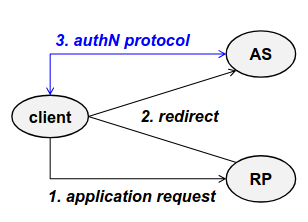
\includegraphics[width=0.5\textwidth]{img/delegated auth.png}
  \caption{Delegated authentication schema}
  \label{fig:delegated-auth}
\end{figure}

At the end of the authN process, the result is transmitted from the AS
to the RP trough various possible ways, which can vary depending on
various factors:
\begin{itemize}
  \item speed, or reaction time
  \item security and trust
  \item on services, interfaces, network filters
\end{itemize}

In the end, there's no best solution, meaning that one have to
evaluate the best solution for the specific case.
\subsection{Possible ticket transmission methods}
Let's now concentrate on the connection between the AS and the RP.
The AS can transmit the ticket to the RP in different ways, which can 
be classified in three main categories.

\paragraph{Push tickets(Figure \ref{fig:push-tickets}):} the ticket is
sent directly from the authentication server to the relying party.
This seems easy but is not that straightforward(think about network 
filters, firewalls, etc).

\paragraph{Indirect push tickets(Figure \ref{fig:inderice push
tickets}):} Since a direct communication between the authentication
server and the relying party may be impossible for various reasons, an
alternative is that the ticket is generated by the authentication
server, given to the client, and then the client will send it to the
relying party. An example of this method is Kerberos.

\paragraph{Push reference + pull tickets(Figure \ref{fig:push 
reference + pull tickets}):} the ticket reference(not the ticket
itself) is sent from the authentication server to the client, and then
from the client to the relying party. Finally, the ticket will be
pulled from the relying party. 

\begin{figure}[H]
  \centering
  \begin{subfigure}{.3\textwidth}
    \centering
    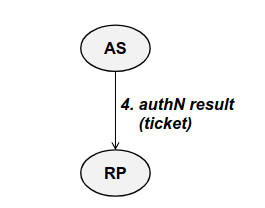
\includegraphics[width=0.9\textwidth]{img/push tickets.png}
    \caption{Push tickets}
    \label{fig:push-tickets}
  \end{subfigure}
  \begin{subfigure}{.3\textwidth}
    \centering
    \includegraphics[width=0.9\textwidth]{img/inderice push
    tickets.png}
    \caption{Indirect push tickets}
    \label{fig:inderice push tickets}
  \end{subfigure}
  \begin{subfigure}{.3\textwidth}
    \centering
    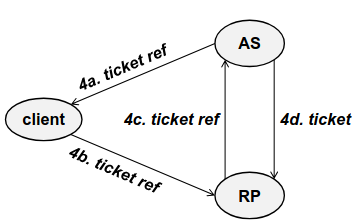
\includegraphics[width=0.9\textwidth]{img/pull ticket.png}
    \caption{Push reference + pull tickets}
    \label{fig:push reference + pull tickets}
  \end{subfigure}
  \caption{Ticket transmission methods}
\end{figure}

\subsection{Problems with tickets}
Each one of those solutions has its own problems:
\begin{itemize}
  \item binding with client, or how to bind the ticket with a 
    specific client and a specific request. If binding is not done
    correctly, replay attacks can be performed.
  \item ticket authentication, or authentication of the server from
    which is the ticket coming from
  \item ticket manipulation (at client). There are cases in which the
    ticket is passed through the client, so the client may alter that
    ticket, if not adequately protected.
  \item ticket manipulation (by MITM)
  \item ticket sniffing (in the network / at client), which exposes
    another concern: privacy!
  \item listening service at RP, which is necessary for the RP to
    listen for incoming tickets
  \item incoming firewall at RP, which can block incoming tickets 
  \item ticket replay (by same client): not only when is bound to a
    client, but also if its coming from the same client(identity
    ticket shared among multi user client)
  \item ticket reuse (at different client): is it tied to the client
    or movable to another client?
\end{itemize}

\subsection{Ticket protection}

Ticket protection is essential for securing the transmission of
tickets between the AS and the RP. 

In the case of the direct transmission between the authentication
server and the relying party, so the case of the push of the
ticket, we have different solutions.
One solution could be the creation a \textbf{digital signature} by the
authentication server that will provide authentication and integrity,
plus encryption of the data with a key possessed by the relying party.
This means full protection of the ticket.
Or if you prefer, one can create a \textbf{secure channel} where the
requirement of the secure channel which security requirements are the
authentication of the AS data integrity authentication, data
encryption and protection against replay.

In case of indirect communication, digital signature provided by the
AS and encryption for the RS is necessary and the only solution to 
protect the ticket.

More in general, protection for replay or reuse requires two things.
First of all, a timestamp, with an associated validity window(as short
as possible to still be usable). Secondly, binding the ticket with the
ID of the user that authenticated, and eventually, its network
address.

\subsection{Federated authentication}

Delegated authentication is typically performed within one single
security environment, typically within a company (like PoliTo), since
there is a very well-known set of users and RPs, and it is possible to
setup one single authentication server and all the relying parties
will delegate to that authentication server the authentication. It
does not work well when we’re in a public system like Internet, in
which we don’t know all the RP and there are several AS.

It is possible to federate the authentication among different security
domains, by using a \textbf{federated authentication system}. The
problem rely in the fact that there are various security domains, each
one managed by a different authentication server so each security
domain, internally, has got delegated authentication mechanism but the
problem is how users from one domain are able to access another
security domain. We need to create \textbf{trust relationship} so that
a relying party belonging to one domain will accept the authentication
performed by the authentication server in another domain. 

When we talk about federated authentication, unfortunately, we change
the terms. The authentication server is typically named IDP
(\textbf{Identity Provider}) while the relying party is named SP
(\textbf{Service Provider}). They are basically the same thing; the
names are related to the context.

\section{XACML}
XACML (eXtensible Access Control Markup Language) is a markup language
derived from XML designed for describing authorization policies and
managing access to protected resources. It defines policies in terms
of:

\begin{itemize}
    \item \textbf{Subject:} Entities such as users, computers, or
      services requesting access.
    \item \textbf{Resource:} Items like documents, files, or data that
      are protected and identified through URIs.
\end{itemize}

XACML also includes a language for managing access requests to these
resources. It specifies:

\begin{itemize}
    \item A structured data format to represent access request and
      response messages.
    \item Transmission over a client-server protocol of choice. After
      all, it's just a language.
\end{itemize}

XACML is an OASIS standard, with its syntax based on XML, making it
widely compatible for authorization tasks in distributed environments.

\subsection{Policy-based access control}
So, the general concept of policy-based access control it’s back to
when the IETF (Internet Engineering Task Force) wanted to have a
common way to describe admission control policies for Quality of
Services on routers. Internet infrastructure is typically multidomain,
since routers are managed by different corporations so it is needed a
common way to describe if a specific request for QoS can be satisfied
or not, after the requestor has been authenticated. So, there was an
original RFC that specified the general framework for policy-based
admission control, and then there was the COPS (Common Open Policy
Service) protocol that tried to implement that concept.

COPS was not very successful but it leaded to the foundation of what
came subsequently. After this initial attempt, there was a
generalization, an extension, to the management of information systems
(by DMTF: Distributed Management Task Force) and to the access control
in distributed environments (work performed by OASIS to apply this
concept to access control in multidomain environments).

\subsection{Components policy-based access control}
The general architecture of XACML is used for other applications, even
though XACML is not used anymore, and it's made up of four components:
\begin{itemize}
  \item  \textbf{PEP = Policy Enforcement Point}: protects a resource
    and allows access only after verification of compatibility with
    the policy
  \item  \textbf{PDP = Policy Decision Point}: receives all the data
    (policy, subject, resource, access type, context) and decides
    whether to permit or deny the access
  \item \textbf{PIP = Policy Information Point}: provides the info
    related to the access requested
  \item \textbf{PAP = Policy Access Point}: provides the policy
    applicable to the requested access
\end{itemize}

 The general architecture of a policy-based access control,
 independent of XACML, is shown if figure \ref{fig:policy access
 control}, and be implemented in several ways.

 Somewhere there is the \textit{policy repository}, where all the
 access policies are stored, which have also been created by a policy
 administrator or security manager using the PAP, which is also in
 charge of retrieving the applicable ones. Then there is a subject
 (user/router/network service) that wants to access an protected
 object. In between the subject and the object to be accessed there is
 the PEP which must decide if this kind of access is permitted or
 denied. Typically, the subject is sending a request in the form of a
 triplet
 (S,O,T):” I am this subject S, I want to access this object O, and
 the kind of access I am requesting is of this type T”. PEP does not
 know if this should be permitted or denied, so in any case it will
 block the initial request and it will talk with an appropriate
 identity: the PDP, the one that is in charge of taking a decision.
 The request MAY be (optionally) enriched with some context
 information (for example, let’s imagine that we need to know what
 time of the day is it, or where the request is physically coming
 from, for example by using geolocalization, or I could see if there
 is a direct connection or if the user is using a proxy, etc.) which
 provides more information about the kind of request and are provided
 by the PIP. Everything is
 then packed together in the form of a XACML request. Now the PDP, in
 order to take a decision, must know which policy is applicable to
 this specific case. It will query the PAP and when it will have that
 policy, it will take the decision and will send back, in XACML
 format, the response. This is mediated by the context handler, which
 has the task of translating that to the language which is understood
 by the PEP. So, finally, the response is provided to the PEP that
 will implement the response: if authorized, it will allow the 
 connection to take place.

\begin{figure}[H]
  \centering
  \includegraphics[width=0.5\textwidth]{img/policy access
  control.png}
  \caption{Policy-based access control architecture}
  \label{fig:policy access control}
\end{figure}

Notice that XACML is limited to the part in yellow in the picture, the
internal communication, because PEP is typically a kind of security
control that already exist and was considered many years ago before
XACML. The typical example of a PEP could be a firewall (network or
application firewall), or it can be any engine inside an application
that must decide if a certain action is permitted or denied, or an
Operating System in which you want to perform some operations on the
files. Those already have their own way to be configured, take
decisions, etc. That’s why normally the context handler is in place,
if not for this part (imagine we don’t need/have that), at least for
translating from a specific request format to the generic XACML. In
the end, the scope of XACML is too small.

\paragraph{Context handler}
The PEP is tightly bound to the application or service (e.g., it can
be a web server or a firewall) and it uses specific formats for
requests/responses (few PEPs are capable of using directly XACML). The
context handler converts access requests/responses from/to XACML and,
if needed, it enhances the requests with the attribute values
(obtained from PIP) often in the form of SAML assertions. When you put
some information, you want to be sure that the information is correct,
so an assertion is a strong statement: “Yes, in this moment it is
14:14:54” and it is possible to prove that, or it is possible to prove
that the user has been authenticated with his username and password.
Some strong foundation to take your decision are needed.

\subsection{XACML policy format}
A \textbf{PolicySet} serves as the primary container in an access
control system, capable of holding individual policies or other nested
PolicySets, allowing for a recursive structure. At its core, a
PolicySet must contain at least \textbf{one policy}, which defines
access control through specific components.

\textbf{Rules} within a policy establish \textbf{conditions} for
granting or denying \textbf{access}. Each rule includes an
\textbf{effect}, which determines whether access is permitted or
denied, and an \textbf{optional condition} that specifies additional
criteria to evaluate. The \textbf{target} of a policy defines its
\textbf{scope} by identifying the circumstances under which it
applies. This involves specifying the subject, the action, and the
resource.

In a Target, \textbf{Subjects} are entities described by
\textbf{attributes}, such as roles, IP addresses, or usernames. This
approach supports Role-Based Access Control (RBAC), a model that
focuses on roles within an organization rather than individual
identities, making it more flexible and scalable. \textbf{Actions}
outline the operations permitted under the policy, such as viewing,
creating, or deleting resources. \textbf{Resources} refer to the
protected entities, typically identified by URIs, that the policy
governs.


\begin{figure}[H]
  \centering
  \includegraphics[width=0.5\textwidth]{img/xacml policy
  format.png}
  \caption{XACML policy format}
\end{figure}

\subsection{XACML request format}

A request in an access control system specifies the subject, resource,
action, and environment, all derived from the request context. Each of
these elements is described through attributes, which provide detailed
information for evaluation.  

The \textbf{resource} identifies the data or object to which access is
requested. It is characterized by a set of attributes that define its
nature and context. The \textbf{action} describes the operation to be
performed on the resource, represented by its associated attributes.
The \textbf{subject} refers to the entity requesting the action,
detailed through its attributes, such as identity or role.  

Attributes serve as the foundation for defining and evaluating access.
Each attribute includes an \textbf{AttributeID}, which uniquely
identifies it, and an \textbf{AttributeValue}, which specifies the
required value for access to be granted or denied. Standard
identifiers, such as usernames, certificate Distinguished Names (DNs),
URIs, and action types, are commonly used to structure these
attributes within the system.


\begin{figure}[H]
  \centering
  \includegraphics[width=0.5\textwidth]{img/xacml request
  format.png}
  \caption{XACML request format}
\end{figure}

\subsection{XACML response format}

The response format in XACML conveys the decision made by the PDP
regarding an access request. This decision is encapsulated in the
result, which includes key elements for interpreting the outcome.  

The decision reflects the outcome of applying the policy to the
request. It can result in one of four possibilities: permit, deny,
indeterminate, or not applicable. An indeterminate decision arises
when inconsistencies or conflicts in the policy prevent a clear
resolution, where access might be both permissible and deniable
depending on the criteria. A not applicable decision indicates that no
relevant policy exists for the specific request.  

The response also includes the status, which provides additional
context about the authorization process. This status contains a status
code, a message detailing the decision, and any associated status
details. Together, these components offer a comprehensive explanation
of the PDP's decision-making process.

\begin{figure}[H]
  \centering
  \includegraphics[width=0.5\textwidth]{img/xacml response
  format.png}
  \caption{XACML response format}
\end{figure}

\section{SAML}

SAML (Security Assertion Markup Language) is a data format used for
handling authorization and authentication assertions. It is designed
to:

\begin{itemize}
  \item Represent different types of assertions.
  \item Construct requests for assertions.
  \item Represent responses containing assertions.
\end{itemize}

Again, the transport protocol is not specified: there is the object,
there is the format of the request, the format for the reply, but
transportation is left to implementation.

The core concept in SAML is the \textbf{Assertion}, which serves as
the base object to convey authentication and authorization decisions.
SAML aims to standardize and simplify interactions required to
establish permissions across a multi-domain distributed system, which
requires trust relationships.

SAML is an OASIS standard with syntax based on XML. It also provides
online tools to encode and decode various SAML formats and messages. A
helpful tool for this purpose can be found at:
\url{https://www.samltool.com/online_tools.php}.

There are various versions of SAML:
\begin{itemize}
  \item SAML 1.0
    \begin{itemize}
      \item november 2002
      \item original version
    \end{itemize}
  \item SAML 1.1
    \begin{itemize}
      \item september 2003
      \item can protect messages with XML-dsig
      \item defines profiles for web browser SSO:
        \begin{itemize}
          \item browser/artifact profile = token SAML by ref
          \item browser/POST profile = token SAML by value
        \end{itemize}
    \end{itemize}
\end{itemize}

Nowadays most of the applications use SAML2.0, which is incompatible
with the previous versions. It can still protect the messages with
XML-dsig, but can additionally use XML-enc for identifiers, attributes
and assertions (the reason is to protect the privacy of the
requestor). In addition to browser/artifact and browser/POST it has
defined new protocols, binding and profiles.


\subsection{Use cases}
Let's start to see the typical cases that have generated the various
usage of SAML.

\subsubsection{Web browser SSO use case}
A web user would like to access a protected resource of the Service
Provider (or relying party). The website does not want to implement by
itself authentication and authorization, meaning that it relies on an
Identity Provider to perform it. This is quite like the Delegated
Authentication that we discussed. This is one of the ways (the most
common) to implement it (e.g., when logging to \texttt{polito.it}, you
are always redirected to \texttt{idp.polito.it} to prove the identity,
and then, it will return an assertion about the authentication). SAML
here is used from the IDP to the SP.

\subsubsection{Authorization service use case}
This use case is very similar to the XACML one: an user is requesting
access to a resource, which access is mediated by a access control
point, the PEP, that will use SAML to check permission with the PDP.
The authorization can be returned in a SAML object (the SAML
response). So, the SAML part is in the way from PDP to PEP.

\subsubsection{Back office transaction use case}
Imagine that a professor at PoliTo want to buy something on behalf of
the university. In order to be able to do so, he must authenticate to
a authority known by both parties and be qualified to perform that
operation, receiving a SAML assertion that he can use to prove that he 
is allowed to do that. 

% 3 images 
\begin{figure}[H]
  \centering
  \begin{subfigure}{.3\textwidth}
    \centering
    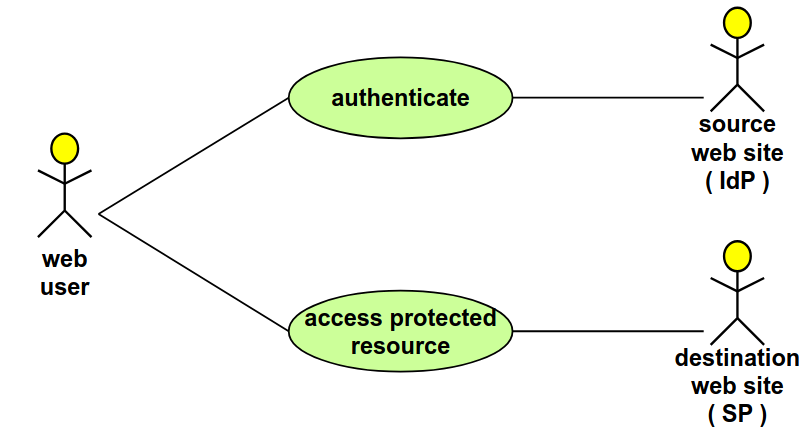
\includegraphics[width=0.9\textwidth]{img/sso use case.png}
    \caption{Web browser SSO use case}
  \end{subfigure}
  \begin{subfigure}{.3\textwidth}
    \centering
    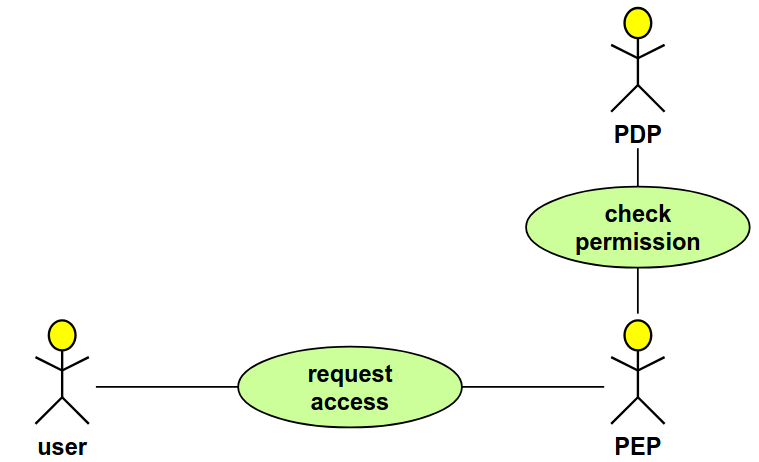
\includegraphics[width=0.9\textwidth]{img/as use case.png}
    \caption{Authorization service use case}
  \end{subfigure}
  \begin{subfigure}{.3\textwidth}
    \centering
    \includegraphics[width=0.9\textwidth]{img/back office use
    case.png}
    \caption{Back office transaction use case}
  \end{subfigure}
  \caption{SAML use cases}
\end{figure}

\subsection{SAML Assertion}

A SAML assertion is a \textbf{declaration of a fact} regarding a
subject, such as the role of a user, made by a specific issuer. There
are three primary types of assertions related to security:

\begin{itemize}
    \item \textbf{Authentication}: confirms the identity of the
      subject. This is the one returned by the Identity Provider (IDF
      – SP)
    \item \textbf{Authorization Decision}: declares whether the
      subject is allowed to access a specific resource. This is for
      the PEP-PDP communication.
    \item \textbf{Attributes}: provides additional information about
      the subject, like roles or permissions.
\end{itemize}

SAML assertions are extensible, allowing for the addition of new
assertion types as needed which can be used in a closed domain.
Additionally, assertions can be digitally signed using XML signature
to ensure authenticity and integrity. Why optionally? Because
assertions can be carried in a secure channel, like an SSL one.

\subsubsection{Information Common to All Assertions}

All SAML assertions contain the following common information:

\begin{itemize}
    \item \textbf{Issuer and Issuance Timestamp} – identifies the
      issuer and the exact time the assertion was issued.
    \item \textbf{Assertion ID} – a unique identifier for each
      assertion.
    \item \textbf{Subject} – includes the subject's name and the
      associated security domain.
    \item \textbf{Conditions} – specifies conditions under which the
      assertion is valid:
    \begin{itemize}
        \item SAML clients must reject assertions with conditions they
          do not understand (just like critical extensions in x.509).
        \item An essential condition is the \textit{assertion validity
          period}, the lifetime of this assertion.
    \end{itemize}
    \item \textbf{Other Useful Information} – may include an
      explanation or proof of the basis on which the assertion was
      constructed.
\end{itemize}

\subsubsection{Authentication Assertion}

An authentication assertion allows an issuer to declare the following
information: \textbf{the Subject S, at time T, was authenticated with
the mechanism M.}

That’s important, because in the previous course we discussed that
there are several authentication mechanisms, and they are not
equivalent: some are strong, some are weak, maybe it is possible to
combine them in a multi-factor authentication, and maybe there are
some Service Providers that will permit access only if strong
authentication has been performed, otherwise will not accept. Since
authentication is outside the control of the SP, because it is
performed by another entity (the IdP), it is needed a way to specify
back to the requestor “Yes, you are authenticated and I tell you that
I used these mechanism”, it is possible to decide if it is strong
enough or not.

\begin{boxH}
  SAML itself \textbf{does not perform the authentication process}
  (such as password requests or challenge-response interactions).
  Instead, it provides a mechanism to link to the results of an
  authentication that has already been completed by an authentication
  agent.
\end{boxH}

Now, take a look at the figure \ref{fig:saml-auth-assertion} to see
how an authentication assertion is structured. As we said, SAML is
just XML, with an opening tag \mintinline{xml}{<saml:Assertion>}. A
version major and minor fields are present, as well as the
AssertionID, which is often in the form of an IP address followed by
the date and time or the serial number. Then there is the Issuer, and
the IssueInstant fields, which will specify the date and time of the
creation (the Z at the end stands for Greenwhich Time). The second
part contains Conditions, for instance, in this case the validity time
frame. Then there is the AuthenticationStatement, which is the of the
authentication. It is made by:
\begin{itemize}
  \item AuthenticationMethod (e.g., password, reusable password, …).
  \item AuthenticationInstant: the date and time in which the user
    interacted with the IdP.
  \item Subject: NameIdentifier + SecurityDomain. Whitin the domain
    polito.it the user with username alioy has been identified.
\end{itemize}
If the issuer is trusted, then it is possible to accept this as a
proof that the user was authenticated. Of course, there are problems
of trust: if that has been manipulated, how it is transmitted, so the
transmission of this SAML token goes back to the discussion of the
previous pages about how to transfer the result of the delegated
authentication.

\begin{figure}[H]
  \centering
  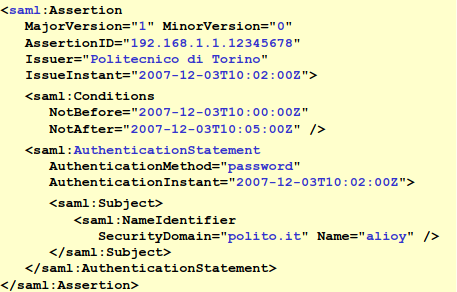
\includegraphics[width=0.6\textwidth]{img/saml auth assertion.png}
  \caption{SAML authentication assertion}
  \label{fig:saml-auth-assertion}
\end{figure}

\subsubsection{Attribute Assertion}

An attribute assertion allows an issuer to declare the following
information: \textbf{the subject S is associated with one or more
  attributes (attributes A, B, C, …) that currently (in this moment)
  have the values “a”, “b”, “c”, … }

\noindent These attributes are typically obtained through an LDAP
query.

\noindent \textbf{Example:} The subject "alioy" within the domain
"polito.it" is associated with the attribute "Department," holding the
value "DAUIN."

Take a look at the figure \ref{fig:saml-attribute-assertion} to see
how an attribute assertion is structured. 
The Initial tag and Conditions are the same as in the previous
example. Then, it is specified that the example is an
AttributeStatement, in which there will be a different content. The
NameIdentifier is the same as before (security domain + name). Then in
the Attribute part there will be the AttributeName “Dipartimento”,
again in the specified namespace (because each namespace may have
different attributes) and the value will be DAUIN. So, if the system
manager is performing Role Based Access Control, it is possible to say
something like “Everybody which belongs to a certain department can
access, for example, the portion of the information system related to
that department”. This is the way in which is possible to know that a
user belongs to that department.

\begin{figure}[H]
  \centering
  \includegraphics[width=0.6\textwidth]{img/saml attribute
  assertion.png}
  \caption{SAML attribute assertion}
  \label{fig:saml-attribute-assertion}
\end{figure}

\subsubsection{Authorization decision assertion}
Finally, to implement the PIP-PDP model, there is the authorization
decision. An issuer declares that \textbf{it has taken a decision
  regarding an access request made by a subject S for an access of
  type T to the resource R based on the evidence E}.

The S, T, R elements are the access request, while the E is important
for taking care of why the permission has been given/denied. For
example, it could as a minimum say “this is based on
polito.it.policy.2.5”, because maybe the policy will change in the
future and by specifying it there will be an evidence that in that
version there was the allowed access to anybody of the DAUIN
department for the resource. The subject can be a person, a program
and a resource can be everything (e.g. a web page, a file, a web
service etc.).

Take a look at the figure \ref{fig:saml-auth-decision-assertion} to
see how an authorization decision assertion is structured. 
The initial tags are the same as before, but in this case there will
be the AuthorizationStatement, in which there will be the decision
field to specify if it is permitted to access the specified resource
(\texttt{http://did.polito.it/m2170.php}) from the person specified in
the Subject (the one corresponding to name alioy in the domain
polito.it). In this case the evidence part is not specified. It means
that the decision has been taken and it is not conveying in the
assertion why the decision has been taken in that way.

\begin{figure}[H]
  \centering
  \includegraphics[width=0.6\textwidth]{img/saml authorization
  decision assertion.png}
  \caption{SAML authorization decision assertion}
  \label{fig:saml-auth-decision-assertion}
\end{figure}

\subsection{SAML producer-consumer model}
These different kinds of assertions are related. By looking at the
last example (authorization decision assertion) it is possible to
notice that the subject is specified, but has the subject
authenticated? If authentication is needed, it means another assertion
is needed.

The assertions can be used individually, but they are quite often used
together, which leads to the general schema presented in figure
\ref{fig:saml produce-consumer model}, in which there are several
entities that at the same time are producing an assertion but also
consuming (receiving) an assertion. 

The schema contains three types of available assertion in the SAML
part. The authentication assertion is from an authentication
authority, the attribute assertion is from an attribute authority but
notice that before deciding which is the attribute it is needed to
know who is the requestor, and the Policy Decision Point is creating
an authorization decision, but this could be based on the identity of
who is requesting and maybe on the attributes (maybe “Lioy” is not
enough, which Lioy? From which department?) and the authorization
decision is used by the \textbf{Policy Enforcement Point}. Each of them (the
authorities) has got a specific policy, for example the
authentication method, and then there is some system entity (which can
be a user, or a program) that performs an application request, the PEP
will block (control) the access to the SP and the system entity in
order to get access must perform authentication (maybe trough a
Credentials Collector or an Authentication Protocol) and then the path
showed in the picture will start.
\begin{figure}[H]
  \centering
  \includegraphics[width=0.6\textwidth]{img/saml produce-consumer
  model.png}
  \caption{SAML producer-consumer model}
  \label{fig:saml produce-consumer model}
\end{figure}

\subsection{SAML: protocol for the assertion}
SAML is not only describing the format of the assertion itself but is
also specifying how the request and the response are created (but not
how they are transported).

The assertion will be contained in a SAML container and will be put in
a Response. The request must be created for that specific type of
assertion, and that is created between the relying party and the
asserting party. It is used “relying party” because it relies upon the
asserting party being a trusted source of information, so it relies on
the assertion created by the asserting party to implement its own
functionality.

\begin{figure}[H]
  \centering
  \includegraphics[width=0.4\textwidth]{img/saml assertion
  protocol.png}
  \caption{SAML assertion protocol}
\end{figure}

\subsubsection{Request of authentication assertion}
The request of authentication assertion is conceptually something of
the kind “please, give me authentication information, regarding this
subject, if you have any”. It is assumed that requestor and the
responder have a trust relation, because they speak about the same
subject and the response is a sort of recommendation letter: “yes, it
is possible to trust this user because I have authenticated it”.

An example of request of authentication assertion is shown in figure 
\ref{fig:saml-auth-assertion-request}.
In the picture the example shows now \mintinline{xml}{<samlp>} where p
stands for protocol. The content will now be an AuthenticationQuery
which asks for information about the specified user. It is something
like: “please tell me if you have authenticated this guy that pretends
to be alioy in the domain polito.it”.

\begin{figure}[H]
  \centering
  \includegraphics[width=0.5\textwidth]{img/saml auth assertion
  request.png}
  \caption{An example of request of authentication assertion}
  \label{fig:saml-auth-assertion-request}
\end{figure}

\subsection{Trust relationship}
The assertion is part of a triangle between to the parties: user, service
provider and the identity provider. 

The one who accepts the assertion must trust the entity that generates
an assertion. The trust relation is established by pushing or direct
pull on a secure channel (e.g., TLS), which may be established with
mutual authentication or at least the asserting party must
authenticate itself. If a TLS channel is not used or if it is wanted
to maintain a proof of the assertion, it is possible to use
XMLsignature over the SAML object using a shared (MAC) or public key
(real digital signature). The last case is a long-term solution while
the TLS channel gives a temporary trust.

\subsection{Binding SAML}
SAML defines \textbf{"what"} to transport, while the binding defines
\textbf{"how"} to transport it, i.e., a network protocol for SAML
requests and responses.

\begin{itemize}
    \item SAML/SOAP(Service oriented architecture protocol)-over-HTTP
      is the original binding in version 1.0.
    \item SAML 2.0 defines other bindings:
    \begin{itemize}
        \item SAML SOAP binding (based on SOAP 1.1)
        \item Reverse SOAP (PAOS) binding
        \item HTTP Redirect (GET) binding
        \item HTTP POST binding
        \item HTTP Artifact binding
        \item SAML URI binding
    \end{itemize}
\end{itemize}

\subsection{SAML Profiles}
A SAML profile is a concrete manifestation of a defined use case using
a particular combination of assertions, protocols, and bindings. 

In practice a profile is like a software pattern (design pattern)
which is a standard way to implement something relative to important
information for a specific use case:
\begin{itemize}
  \item Web browser profile is needed to implement Single Sign On
    (SSO) web
  \item SOAP profile is used for assertion about the SOAP payload – in
    case it is used
\end{itemize}

\subsection{SAML and SOAP}
Typically, we have SAML that contains a SOAP message with the SOAP
header, SOAP body, and the request and response are carried inside
this protocol. So it actually is layered in three protocols: SAML
inside SOAP inside HTTP.

Figure \ref{fig:soap-profile} shows how the SOAP profile is 
structured. 

% 2 subfigure 
\begin{figure}[H]
  \centering
  \begin{subfigure}{.4\textwidth}
    \centering
    \includegraphics[width=0.9\textwidth]{img/soap over http.png}
    \caption{SAML over SOAP over HTTP}
  \end{subfigure}
  \begin{subfigure}{.4\textwidth}
    \centering
    \includegraphics[width=0.9\textwidth]{img/soap assertion.png}
    \caption{SOAP profile}
    \label{fig:soap-profile}
  \end{subfigure}
  \caption{SAML and SOAP}
\end{figure}


\subsection{Web Browser Profiles}

Web browser profiles, which are surely more relevant nowadays, operate
under the following assumptions:
\begin{itemize}
    \item A standard commercial browser and HTTP(S) are used.
    \item The user has authenticated with a local source site.
    \item The assertion’s subject implicitly refers to the user.
\end{itemize}

When a user tries to access a target site:
\begin{itemize}
    \item A small authentication assertion reference is included with
      the request, allowing the real assertion to be dereferenced.
    \item Alternatively, the real assertion is directly POSTed.
\end{itemize}

The choice between these methods is determined by the agreement
between the Service Provider (SP) and Identity Provider (IdP).

\subsection{SSO use case}
\subsubsection{SSO push use case}
The procedure is shown in figure \ref{fig:sso-push-use-case}. The the
client (browser) is trying to connect  to a specific page of a web
server (which is the SP). The resource is protected, so a redirect is
received (HTTP codes that start with 300). The SP has a specific
agreement with an Identity Provider like the case of PoliTo and is
redirecting there with an authentication request, which is hidden
inside the redirect. It means that when the client goes to the
Identity Provider it is automatically transmitting this authentication
request (number 3 in the picture) which is not created by the client,
but it is a consequence of the redirect.

The Identity Provider is implementing some kind of authentication
protocol (username and password, OTP, challenge response etc.) and
will finally create the answer and it must return the answer to the
Service Provider.


Assuming that it is successful, then will create for you a form that,
when you hit the Submit button, will send you to the service provider.
Inside this form, as hidden data, there will be the authentication
result. When the client wants to go back to the Service Provider, it
will automatically (involuntarily) transmit the authentication
response (number 6, again it is not created by the client). This is
the push use case (with reference to the delegated authentication),
because the IdP is pushing the token (which is the SAML assertion) to
the SP. Finally, the SP (if authN was successful) will provide the
requested service to the client.

It is also named front-channel exchange because it directly uses the
channel towards the SP.

\begin{figure}[H]
  \centering
  \includegraphics[width=0.5\textwidth]{img/sso push use case.png}
  \caption{SSO push use case}
  \label{fig:sso-push-use-case}
\end{figure}

\subsubsection{SSO pull use case}
In the SSO push use case all data are transmitted using the same port
(there will not be an alternate port).

In this case, the first stages are the same as before: service
request, redirect to IdP, authentication request (passed as a GET
parameter), authentication protocol and then the difference. The step
number 5 is changed: here there is now a redirect (a GET) with an
artifact, which is a pointer to the result. The client will pass the
artifact to the SP, which will need to open a direct channel to the
IdP and to perform an authentication result request. Then the IdP will
sent the authentication result and if it is positive the SP will
provide to the client the requested service.

This case is named pull because in the response it is passed the
pointer, and the SP needs to go and pull (take) the response from the
IdP. This case could be better than the previous one because, for
example, it does not require any signature. Assuming that the
communication channel between SP and IdP is based on TLS, with TLS
authentication for the IdP, then the SP can be sure of the result even
without a signature of the signature. Of course, if the SP will need
in the future to demonstrate the assertion, that could not be possible
since it is not signed.

This use case is simpler (keys or certificates are not needed) but it
takes a bit more time because it is needed to open a separate network
channel. If a lot of authentications is performed, it is possible to
keep the TLS channel always open, so it is just needed a RTT to
perform the request and get response, but there will not be the
overhead of opening the channel. Finally, there is a problem on the
IdP if there is an incoming firewall. 

It is also named artifact binding or back-channel exchange because
another channel is needed. 

\begin{figure}[H]
  \centering
  \includegraphics[width=0.5\textwidth]{img/sso pull use case.png}
  \caption{SSO pull use case}
\end{figure}

\subsection{SAML SSO for Google Apps}
This kind of architecture is being used by large providers such as
Goggle to implement SSO for Google Apps.

Google Apps are applications that are hosted by Google, but the
authentication and the authorization are managed by the company that
developed the app. The company asks to Google to run applications on
Google but with the possibility to manage the authentication (so the
company does not want to use Google authentication) in order to keep
control on who is accessing”. This can be performed using SAML.

A company, basically a Google Partner, installs its own applications
on Google (which will be just a service provider). The Partner wants
to maintain control of the authentication and authorization part
(basically the company wants to be an Identity Provider). The exchange
is based on SAML-2.0 with XML signature: this is important because
here there are two difference companies and Google wants to be sure
that any mistake about the authentication cannot be on charge of
Google. This is the typical case in which a signature is needed,
typically a digital signature with X.509 certificate, because in case
of any commercial discussion or legal discussion between Google and
the company, Google wants to have a proof of why they permitted access
to the application.

Basically, there is Google with the Application. All the users that
want to use the application are redirected to the company. Then there
will be the SAML assertion sent to Google which must be digitally
signed, since that is the message that gives access to the application
from Google to the user. If an assertion is accepted without any
signature (or with a symmetric signature), then there is no way to
prove that.

\begin{figure}[H]
  \centering
  \includegraphics[width=0.7\textwidth]{img/google sso.png}
  \caption{SAML SSO for Google Apps}
\end{figure}

The partner must provide to Google the URL of the single-sign-on
service that can be also named the IDP, or the Authentication Server,
as you prefer, and the X.509 certificate to verify the signature.
Because the answer is signed with a real public key. Step three
contains, in opaque mode, the URL of the Google service requested by
the user. So the company knows not only, I have to authenticate, they
can also perform authorization. Because this user is trying to use
this service, the SML authentication request. And the URL where to
send the response. And step six, in opaque mode, contains still the
URL of the Google service to avoid a reply.
  
\section{Federated Identity}

So far, we have seen \textbf{Delegated Identity}, which operates
within the same security domain. For example, in the case of PoliTo
(where 100 servers delegate authentication to \texttt{idp.polito.it})
or Google’s delegated authentication model, the authentication is
handled by a specific Identity Provider (IdP) for a specific
application. This setup always involves a one-to-one mapping: one
application corresponds to one IdP. While the same IdP can serve
multiple applications, there is still a 1:1 mapping.

On the other hand, \textbf{Federated Identity} enables multiple IdPs
to interact with the same application service. This is a common
scenario, such as when creating an account on a website where users
can either create a new username and password or authenticate using
Google or Facebook credentials. This federation allows authentication
performed by an external service (outside the security domain) to be
automatically recognized. A key advantage is avoiding
\textit{duplicate authentication}, which can be inconvenient for
users.

Federated Identity extends federated authentication by incorporating
\textbf{identity-related attributes}. SAML is frequently used for
building federated identity systems because it supports both
authentication and attribute assertion. Identity involves more than
just authentication; it includes \textit{authentication + attributes}
(e.g., name, surname, student ID, residence, etc.).

SAML is XML-based. While XML is \textit{simple but heavy}, SAML is
typically suited for PC or server-based environments. However, its
complexity makes it challenging to use in lightweight or mobile
contexts.

There is a juxtaposition between \textbf{SAML} and \textbf{OpenID
Connect}. While SAML works well for server environments, it is less
mobile-friendly. OpenID Connect, on the other hand, provides a similar
architecture involving the client, Service Provider (SP), and IdP, but
it uses \textbf{JSON} instead of XML and relies on the \textbf{REST
protocol}. This makes OpenID Connect more suitable for mobile and web
applications.

\begin{boxH}

\textbf{Beware:} \textit{OpenID 1.0} and \textit{OpenID 2.0} are
\textbf{not} the same as OpenID Connect. The latter is based on
\textbf{OAuth 2.0}, an IETF authorization framework. This distinction
is critical, as the terminology surrounding OpenID can sometimes be
confusing.

\end{boxH}

\subsection{OpenID Connect}
OpenID Connect(OIDC) is a delegated authentication system (the
federated aspect rely in the fact that it support many IdPs).

It uses JSON data and REST protocol(which are native in smartphone
environments), and it is not correlated to OpenID-2.0 but this is an
identity layer put on top of Oauth-2.0 (IETF authorization framework).
It should be the reverse: first authentication then authorization, but
not in this case.

The user agent can be a normal browser o can be a mobile app, beware
of the terms because the client is not the user agent, the client is
the relying party (application server) that wishes to use
OpenID-Connect for authentication.

In this schema the user has its mobile phone, and it is named User-
Agent, which is connecting to an application server, which is the
client, because it is the client of OpenID-connect, connecting to a
server that will provide authentication, authorization, and
attributes. That’s why it is named client because it is the client for
OpenID-connect.

The server S is not a single server, but it is a collection of
servers, or as a minimum a collection of endpoints. It means that when
there is a server with a certain network address, there may be several
different ports or even if everything is on port 80 or port 443, when
performing a GET or POST a path is specified, and that is an endpoint.
There may be \texttt{/authenticate}, \texttt{/authorize},
\texttt{/attributes}: these are different entry points in a REST
application.

Notice that the server, which is the OpenID-Provider (OP), which is
conceptually similar to the IdP, has various endpoints:
\begin{itemize}
  \item Authorization endpoint ($\text{AuthZ}_{EP}$: it is called
    authorization, but it performs authentication (confusing).
  \item Token endpoint ($\text{Token}_{EP}$), something that verifies
    if a certain token generated during the protocol is valid or not.
  \item UserInfo endpoint ($\text{UserInfo}_{EP}$), if the user has
    given the consent, then the client can retrieve information about
    the user.
\end{itemize}

\subsubsection{User authentication}
The login workflow is shown in figure \ref{fig:openid-connect} and is
as follows.

We have the user interacting through a \textbf{user agent}, like a
mobile app or a browser. The \textbf{client} here is the relying party
(RP)—for instance, a web application or a service accessed via the
app. The user begins by choosing to log in using an external IdP, such
as Facebook or Google.

The client generates an \textbf{authentication request} to the IdP.
This request is sent to the IdP’s \textbf{authorization endpoint}, even
though the goal is authentication (this dual-purpose endpoint can
cause some confusion). The request includes details like the client
ID, redirect URI, and requested scopes.

Upon receiving the authentication request, the IdP validates it. This
validation ensures that:

\begin{itemize}
  \item The client (RP) is registered with the IdP (a trusted
    relationship exists).
  \item The request is properly signed and formatted, verifying it
    genuinely comes from the registered client.
\end{itemize}

If the request is valid, the IdP generates an \textbf{authentication
page}. Here, the user enters their credentials (e.g., username and
password). The credentials are submitted back to the IdP’s
\texttt{/authenticate} endpoint, where they are verified.

Once authenticated, the IdP often presents the user with an
\textbf{authorization page}. This page asks the user to consent to the
RP accessing specific data (e.g., profile, email). For example, when
using Google or Facebook login, you might see a message like, "This
app will receive your name, email, and profile picture." 

If the user grants consent, the request is finalized at the
\texttt{/authorize} endpoint. The IdP issues an \textbf{authentication
response}, typically as an ID token (a JSON Web Token, or JWT), which
contains the authenticated user’s information. This token is sent back
to the client via the redirect URI specified earlier.

\subsubsection{Login with token}
The login workflow is shown in figure \ref{fig:openid-connect} and is 
as follows.

It's assumed that the user has already authenticated with the IdP and 
has an active session.
After the redirect from the Authorization Endpoint (AuthZEP), a 
\texttt{GET} request is sent to a \texttt{/callback} endpoint, passing 
the received information. The Authorization Endpoint provided a token 
in response. This token is then handed to the client, which can use it 
at the Token Endpoint (TokenEP) for validation. This demonstrates that 
the user consented to transfer their data to the client. 

The Token Endpoint verifies the token, and if valid, it returns 
\textbf{IDT} (Identity Token) and \textbf{ACCT} (Accessory Information). 
The client verifies the IDT, and if accessory information is present, 
the \textbf{UserInfo Endpoint} (UserInfoEP) may optionally be accessed 
to retrieve additional user details. 

Finally, a successful login occurs, and the client is provided with 
the user's identity and any additional information.

%2 subfigure 
\begin{figure}[H]
  \centering
  \begin{subfigure}{.49\textwidth}
    \centering
    \includegraphics[width=0.9\textwidth]{img/oicd user auth.png}
    \caption{User authentication}
  \end{subfigure}
  \begin{subfigure}{.49\textwidth}
    \centering
    \includegraphics[width=0.9\textwidth]{img/oicd token login.png}
    \caption{Login with token}
  \end{subfigure}
  \caption{OpenID Connect}
  \label{fig:openid-connect}
\end{figure}

\subsubsection{Trust, security and discovery}
All the messages are authenticated with digital signatures, that
requires registration of the public keys among the various actors. All
the messages are protected via secure channel (TLS) but this is not a
real federation, it is just the fact that it is possible to use more
than one. There is a proposed service, WebFinger, to discover the
OpenID Providers but that works only if the provider registered itself
with WebFinger, so it is not much used. But in any case, OpenID
Connect is much used, OIDC providers: Google, Facebook, Salesforce.

\subsubsection{OIDC standard claims}
When additional information about user is requested, it is possible to
ask for:
\begin{itemize}
  \item profile category: subject (ID at the issuer), name (full),
    given\_name, family\_name, middle\_name, nickname,
    preferred\_username, gender, birthdate, zoneinfo, locale, profile
    (URI), picture (URI), website (URI), updated\_at (last update at the
    issuer)
  \item email category: email, email\_verified (Boolean)
  \item phone category: phone\_number, phone\_number\_verified (Boolean)
  \item address category: address
\end{itemize}
When a client is requesting a claim, it may request a single item or a
whole category (e.g., profile category or only family\_name). Apart
from the ones with \_verified=TRUE all the others are self-asserted by
the user and hence unreliable. This is the bad part: the user can be a
fake user. Custom claims can be created, but they have a restricted
audience.

\subsubsection{JWT for claims – example of ID token}
There is: the subject, the issuer (the OpenID connect at PoliTo), the
audience (which client, it can be also www.unito.it because that
server can be a client to accept the user of PoliTo rather than
forcing them to have an account at that website), the nonce, the
authentication time, the authentication context class reference (it is
a way to explain which kind of authentication was performed, of course
some values must be agreed which could be PoliTo, loa stands for level
of assurance and hisec could be high security but there should be a
meaning, a definition behind that), the issued at (at what time the
token was created), the expiration (when it will expire).

\begin{figure}[H]
  \centering
  \includegraphics[width=0.5\textwidth]{img/oicd token.png}
  \caption{Example of ID token}

\end{figure}

\section{eIDAS}

\textbf{eIDAS}, stands for \textit{electronic IDentification, Authentication, 
and trust Services for electronic transactions in the internal
market}, and it's based on the EU regulation 910/2014.

The key point is that in each European country there is a different
identity system (in Italy SPID) but in the same way in which the
identity card, the driving license, the passport is valid also on
abroad, the European Union wanted to allow the use of the electronic
identity when accessing services in a different European country. It
took a lot of years (more then 10 years) and it works and it is used
all over Europe.

Initially, the eIDAS electronic identification (eID) infrastructure was 
voluntary. However, starting from September 2018, it became compulsory for 
EU public services. Adoption by the private sector remains optional but is 
strongly encouraged.

The purpose is to boost confidence and trust towards digital world by
adopting the following principles among others:
\begin{itemize}
  \item Mutual acceptance of national e-ID: all the members of EU are
    trusted
  \item Common framework for secure interaction between citizens,
    companies, and public administration
  \item Technological neutrality of requirements Required to not
    restrict to specific solutions (some countries use smartcards,
    others OTP, etc.). All the solutions are mutually recognized, but
    it is not possible to say all the methods are equivalent.
  \item Level of trust in national electronic identity can be defined
    by a certain e-ID quality level
  \item Country-specific supervision organizations to verify the
    Regulation adoption and interact with the European Commission
    (e.g., for data privacy)
\end{itemize}

There were various implementing acts made by Commission Implementing
\begin{itemize}
  \item 2015/296 (24 February 2015): eID procedural arrangement for
    MS(Member state) cooperation
  \item 2015/1501 (8 September 2015):  interoperability framework
  \item 2015/1502 (8 September 2015): technical specifications for
    assurance levels for electronic identification means
  \item 2015/1984 (3 November 2015):  formats and procedures for
    notification
\end{itemize}

\subsection{Pan-European eID}
Notice once again that identity is not just authentication, it is
\textbf{authentication plus attributes}. The very important point is
the fact that with eIDAS there are certified attributes. In OpenID
Connect there are a lot of information, but only phone number and
email can be trusted, since all the others are self-declared by user.
On the contrary, in eIDAS, since the information is provided by the
government it is trusted. 

So, again in eIDAS there will be e-identity with authentication +
certified attributes
\begin{itemize}
  \item Set of certified European attributes
  \item Lexicon (multilanguage attribute names): it is a problem,
    since all the countries in the EU must agree (due to different
    alphabets and characters).
  \item Syntax (possible values)
  \item Semantics e.g., surname in Italy is just one given by the
    father but in Island there are two surnames, since each person
    keeps both surname of father and mother and they can decide to use
    one or the other. So, it is needed to understand the different
    meaning that even simple things may have in different countries.
\end{itemize}

It is possible to use various authentication credentials such as
reusable password, one-time-password, cellphone, software certificate,
smart-card since the system is technology neutral. The point is that
it is used in a transparent way and with legal value (according to the
citizen’s country).

\subsection{Adaptive security and privacy protection}
Everything is accepted but each authentication method it is assigned
various authentication levels and the authentication level is
attributed through the LOA (Level of Assurance) which means how much
the result (on the authentication method) can be trusted. LOA consists
in three different levels: substantial, medium, high. This is not only
related to the cryptographic strength of the authentication technique,
but also on the strength of the identification process, because e.g.,
a country is using a smart-card with a PKC asymmetric
challenge-response which is the strongest authentication, but how does
the smart-card is given to the citizen? If there is no identification
of the citizen, then it is bad. In the end, the LOA tests both things
in order to give a level to the whole procedure.

When accessing a service there may be a mismatch (e.g., a service is
for transferring money so an High LOA is wanted) if the procedure
provides a Medium LOA but the service requires an High LOA, so
authentication may fail.

For privacy protection and localization, the user talks with its own
country and before transferring attributes abroad, it must provide
explicit consent for the required attributes. The attributes are
managed end-to-end, which means that attributes are transferred from
the government of a country directly to the Service Provider in the
other country: eIDAS infrastructure itself does not store any personal
data. There is minimal disclosure, in the sense that on the contrary
to OpenID Connect in which everything can be requested, in this case
it is applied the Need-To-Know principle, e.g., some services are
reserved to people with age major than 18: in this case the birth date
is not requested, since the service is not interested to that
information but the service will ask to the system if the user is
above 18 or not.

\subsection{eIDAS terminology}
The MS is the Member State. It can be:
\begin{itemize}
  \item Sending MS: it is the MS whose eID scheme is used in the
    authentication process, and sending authenticated ID
  \item Receiving MS: it is the MS where the RP requesting an
    authentication (service that citizen is trying to access) is
    established
\end{itemize}
Then there is an eIDAS-Connector, which is a node requesting a
cross-border authentication and the eIDAS-Service which is a node
providing cross-border authentication. Unfortunately, there are two
implementations.

One big country in Europe did not want to agree with the others, so
99\% of countries implements the eIDAS- Proxy-Service (an eIDAS-Service
operated by the Sending MS and providing personal identification data)
schema, while one country is implementing it using
eIDAS-Middleware-Service (an eIDAS-Service running Middleware provided
by the Sending MS, operated by the Receiving MS, and providing
personal identification data) schema.

\subsection{eIDAS infrastructure}
Imagine to be an Italian citizen with SPID identity that needs to
access a SP in Sweden. The SP will ask to the citizen to choose
between the Swedish identifier or eIDAS for authentication. The
citizen will of course choose eIDAS, so it will be redirected to the
Swedish eIDAS Connector (which connects that country to the rest of
the infrastructure). It will ask to select the country of the citizen
and will then redirect to the Italian eIDAS Service which is
implemented as a proxy. At this point the proxy will provide to the
citizen all the information that Sweden requested (name, surname, date
of birth) and will ask for a preliminary consent (otherwise the
process will stop). Then, since in Italy there are different systems
for identity (SPID, but with many providers such as Poste Italiane and
it could be possible to use the electronic identity card) the citizen
must choose which electronic identifier (e-ID) to use. In this way the
citizen will be redirected to that specific provider, which has got
the identity and the attributes (IDP + AP). At this point, the
authentication will be performed according to the system selected and
there will be a final consent to transfer abroad the specified
information (again name=”Antonio”, surname=”Lioy”, etc.).

\begin{figure}[H]
  \centering
  \includegraphics[width=0.5\textwidth]{img/eidas infrastructure.png}
  \caption{eIDAS infrastructure}
\end{figure}
\subsection{eIDAS technical specifications}
Technical specifications are evolving over the time: Version 1.0
(26/01/2016), 1.1 (16/12/2016), Version 1.2 (27/09/2019). They are all
publicly available on the European website. The protocol is based on
STORK1 and then STORK2, that are developed and tested infrastructure
and finally after STARK2 everything was adopted as the official eIDAS
Infrastructure. It is similar, but not compatible, e.g., in the real
implementation it has been added the encryption of authentication
response to guarantee privacy against network sniffing. It covers, but
only for the international part, i.e., MS-to-MS. Looking the previous
picture, eIDAS in the part 3 (Connector exiting from one country and
the proxy accepting request from the other country). Specification is
only for this part (how SPID works in Italy it is decided by Italian
Government, …). eIDAS is end-to-end conceptually, in the sense that
the response will directly transfer to the SP but as a protocol, it is
only for connecting the end-points at the borders of the various
countries. It covers, only for the international part, the:
\begin{itemize}
  \item Interoperability architecture
  \item SAML message format
  \item SAML attribute profiles
  \item Cryptographic requirements
\end{itemize}
\subsubsection{eIDAS Minimum Data-Set}

The eIDAS regulation specifies a minimum data-set that must be supported by any eIDAS node to enable cross-border authentication. This data-set includes attributes for both natural and legal persons.

For \textbf{natural persons}, the data-set includes:
\begin{itemize}
    \item \textbf{Mandatory Attributes:}
    \begin{itemize}
      \item \texttt{PersonIdentifier}, \texttt{FirstName},
        \texttt{FamilyName}, \texttt{DateOfBirth}
    \end{itemize}
    \item \textbf{Optional Attributes:}
    \begin{itemize}
        \item \texttt{BirthName}, \texttt{PlaceOfBirth},
          \texttt{CurrentAddress}, \texttt{Gender}
    \end{itemize}
\end{itemize}

For \textbf{legal persons}, the data-set includes:
\begin{itemize}
    \item \textbf{Mandatory Attributes:}
    \begin{itemize}
        \item \texttt{LegalName}, \texttt{LegalPersonIdentifier}
    \end{itemize}
    \item \textbf{Optional Attributes:}
    \begin{itemize}
        \item \texttt{LegalAddress} , \texttt{VATRegistration} ,
          \texttt{TaxReference} , \texttt{BusinessCodes} ,
          \texttt{LEI} (Legal Entity Identifier) , \texttt{EORI}
          (Economic Operators Registration and Identification) ,
          \texttt{SEED} (System for Exchange of Excise Data) ,
          \texttt{SIC} (Standard Industrial Classification)
    \end{itemize}
\end{itemize}

\subsubsection{Security Requirements}

\begin{itemize}
    \item \textbf{SAML request} (no personal data) \textbf{MUST} be
      signed with a digital signature, but no encryption is required.
    \item The request may be transmitted via:
    \begin{itemize}
        \item \textbf{HTTP Redirect}: For example, a 302 GET with the
          request in a parameter. This is preferred if the size of the
          request does not exceed the maximum URI length (256
          characters).
        \item \textbf{HTTP POST}: For example, a form with POST and
          the request in a hidden field. This is preferred if the
          request is much larger.
        \item Note: The size of the request can change based on the
          data requested. For instance, authentication requests with
          attributes will make the request larger.
    \end{itemize}
    \item \textbf{SAML response} (containing personal data)
      \textbf{MUST} be signed with a digital signature and must
      include an \texttt{EncryptedAssertion} with:
    \begin{itemize}
        \item One \texttt{AuthenticationStatement}
        \item One \texttt{AttributeStatement}
    \end{itemize}
    The response itself is not encrypted, but portions of it may be
    encrypted as allowed in SAML.
    \item The response is transmitted via \textbf{POST binding} to the
      ACS (\textit{Assertion Consumer Service}) of the connector.
    \item The connector metadata must contain:
    \begin{itemize}
        \item The \textbf{encryption certificate} and \textbf{ACS URI}.
        \item For example, when Italy sends back encrypted data, it
          needs to know the public certificate and the ACS URI to
          perform a redirect after authentication. These details are
          included in the metadata.
    \end{itemize}
\end{itemize}

\textbf{All communication channels must use TLS version $\geq$ 1.2,
with qualified web certificates.} The supported TLS ciphersuites are:
\begin{itemize}
    \item ECDHE+ECDSA or ECDHE+RSA or DHE+DSA (accepted for backward
      compatibility)
    \item AES\_128\_CBC/GCM with SHA256 for encryption
    \item AES\_256\_CBC/GCM with SHA384 for encryption
    \item SHA1 MAY be accepted but only due to restrictions of the
      client browser
\end{itemize}

Other Requirements for TLS:

\begin{itemize}
    \item For \textbf{ECDH keys}, the minimum key size is 256 bits,
      while for \textbf{DH keys} the minimum is 2048 bits.
    \item The \textbf{TLS compression} \textbf{SHOULD NOT} be used.
    \item \textbf{TLS heartbeat} and \textbf{Session Renegotiation}
      \textbf{MUST NOT} be used.
    \item If a \textbf{CBC-based cipher suite} is used, first encrypt
      and then authenticate the data (e.g., use the Enc-then-MAC
      extension).
    \item \textbf{DON'T} use a truncated HMAC (e.g., unsupported that
      extension).
\end{itemize}

Requirements for SAML:

\begin{itemize}
    \item \textbf{Data encryption} only via \texttt{AES-128/256-GCM},
      but \texttt{AES-192-GCM} may also be used.
    \item \textbf{Key encryption} with \texttt{RSA-OAEP-MGF1P} or
      \texttt{RSA-OAEP} (3072 bits minimum key length).
    \item \textbf{Key agreement} via \texttt{ECDH-ES}:
    \begin{itemize}
        \item \texttt{ES} is \textit{Ephemeral-Static mode} (i.e., the
          recipient has static DH parameters while the sender creates
          ephemeral ones). The destination publishes in the metadata
          what its own DH parameters are, while the sender will create
          the ephemerals.
    \end{itemize}
    \item \textbf{Key wrapping} via \texttt{KW-AES-128/256}.
    \item \textbf{Digital Signature} via \texttt{RSAPSS} (3072 bits
      minimum key length) or \texttt{ECDSA} (256 bits minimum key
      length) with \texttt{SHA-256/384/512}.
    \item The trusted EC are: \texttt{BrainPoolP256r1,
      BrainpoolP384r1, BrainpoolP521r1, NIST Curve P-256, NIST Curve
    P-384, NIST Curve P-521}.
\end{itemize}

\subsection{eIDAS 2.0}

eIDAS 2.0 introduces a new schema based on the \textbf{EUDI} (EU
Digital Identity) wallet. It implements the concept of \textbf{SSI}
(Self-Sovereign Identity). The EUDI wallet will provide identification
and authentication, as well as the verifiability of the validity of
the evidence by third parties throughout Europe. It ensures secure
storage and presentation of verified identities and their data, and
enables the generation of qualified electronic signatures.


\section{SPID}
SPID is the Italian Public System for Digital Identity. It's
architecture is based on three main components:
\begin{itemize}
  \item \textbf{Identity Provider (IdP)}: the entity that provides
    digital identity to the user. It is responsible for the
    authentication process and the enrollment of the user.
    It also returns the user identity plus some basic attributes(not
    all of them).
  \item \textbf{Service Provider (SP)}: the entity that performs
    access control based on the identity and attributes. 
  \item \textbf{Attribute Authority (AA)}: the entity that provides
    the user's attributes based on the identity. This is necessary
    there are some attributes that are not controlled by the
    government, for instance the enrollment to the \textit{Ordine
    degli Ingegneri}.
\end{itemize}

\subsection{Protocols and data}
SPID uses SAML version 2 with the web browser SSO profile for data
exchange. The caveat is that each entity prodives its own metadata,
containing:
\begin{itemize}
  \item its X.509 signature certificate, which may be self-signed!
    This is possible because the metadata is public and can be 
    accessed from a goverment controlled website.
  \item its protocol endpoints
  \item various other data (e.g. supported attributes)
\end{itemize}

The metadata are signed by the Agency for Italian Digitalization in
detached form. This means that they will be the target of electronic
signatures. The official metadata registry containing all the service
providers and identity providers can be found at 
\url{https://registry.spid.gov.it/metadata}. The specification in case
of spid are a little bit behind the eIDAS, because the basic signature
algorithm is RSA-2048 with sha-256, while eIDAS requires RSA-3072 
with sha-384.

In case of an HTTP redirect, the SAML request is passed in the query
string of a GET. But this has a limit of 256B for the basic URI, but
typically length of 2kB up to 8kB are supported. Since POST requests
are not to be used, the SAML request is compressed with DEFLATE 
algorithm and not signed with SMLDSIG, but the SigAlg parameter is
used to specify the signature algorithm, in a Base64 url encoded form
of the whole query string. When using HTTP POST, then we permit normal
SAML with normal XML signature.

There are many basic attributes, and each SP may require a specific
attribute set, which groups them. A common example of an attribute set
could be (name, familyName,  fiscalNumber, email).

There are also different authentication levels:
\begin{itemize}
  \item SPID Level 1: the user is authenticated with a password
  \item SPID Level 2: the user is authenticated with a password and OTP
    or password and an app
  \item SPID Level 3: this level requires 2FA with asymmetric authN
    via a secure device, for example a password with an app for remote
    digital signature and a Layer 3 pin
\end{itemize}

\subsection{SPID evolution}
The Attribute Authority is not yet implemented, but it's not for a
technical issue, but an organizational one: the government has not
decided who is authorized to create some attributes.

There's also a requesto make SPID available not only with SAML, but
also with OIDC, to make it more compatible with the rest of the world.
This is compulsory for the IDPs since May 1, 2022. For the service
provider, it is optional to support that.


\section{Q\&A}
\subsection*{Question 1}
what role does the Authentication Server (AS) play?
\begin{itemize}
  \incorrect provides authorization decisions for the RP
  \correct performs authentication on behalf of the Relying Party (RP)
  \incorrect verifies the identity of the RP
  \incorrect issues a session timeout for the RP
\end{itemize}

\subsection*{Question 2}
\begin{itemize}
  \incorrect relaying party is A. the entity that directly authenticates the user 
  \incorrect  the server that stores user credentials
  \correct  the entity that trusts another server to handle authentication
  \incorrect  the client application used by the user
\end{itemize}

\subsection*{Question 3}
the Authentication Server (AS) interacts with the client using
specific protocols to perform authentication. What amongst the
following can be used for the authentication process
\begin{itemize}
  \incorrect HTTP 
  \correct OAuth 
  \incorrect FTP
  \incorrect SMTP 
  \correct SAML 
  \incorrect SOAP
\end{itemize}

\subsection*{Question 4}
how does the Authentication Server (AS) typically
communicate the authentication result to the Relying Party (RP)?
\begin{itemize}
  \incorrect  by issuing an authorization code 
  \incorrect  by sending a cookie
  \correct  by providing a ticket or assertion 
  \incorrect  by creating a session ID
\end{itemize}

\subsection*{Question 5}
Which of the following scenarios best represents a delegated authentication setup in a Single Sign-On (SSO) environment
\begin{itemize}
  \incorrect  the user logs in separately to each application with the same credentials
  \correct the user logs in once, and a central AS authenticates them for multiple RPs
  \incorrect each application has its own AS that verifies the user separately
  \incorrect the user must verify their identity with each RP individually
\end{itemize}

\subsection*{Question 6}
Which format is commonly used to provide assertions in delegated authentication systems like SAML?
\begin{itemize}
  \incorrect  JSON Web Tokens (JWT)
  \incorrect  Hypertext Markup Language (HTML) 
  \correct  Extensible Markup Language (XML) 
  \incorrect  Simple Mail Transfer Protocol (SMTP)
\end{itemize}

\subsection*{Question 7}
Which of the following is a key benefit of using delegated authentication for a Relying Party (RP)?
\begin{itemize}
  \incorrect  reduced dependency on external servers 
  \correct  enhanced data privacy for user credentials 
  \incorrect  increased complexity in user management 
  \incorrect  independent authentication for each RP
\end{itemize}

\subsection*{Question 8}
what does a SAML assertion represent?
\begin{itemize}
  \correct  declaration of a fact about a subject, like user information
  \incorrect  a statement about of how often a user logs in
  \incorrect  a protocol for secure email communication
  \incorrect  a form of encryption used for securing passwords
  \incorrect  a method of encoding data in XML format
  \correct  declaration made by an issuer about a different subject
\end{itemize}

\subsection*{Question 9}
Which of the following is not a standard type of SAML assertion?
\begin{itemize}
  \incorrect  authentication assertion
  \correct  Service type assertion
  \incorrect  authorization decision assertion 
  \correct  public key certificate assertion 
  \incorrect  attribute assertion
  \correct  token assertion
\end{itemize}

\subsection*{Question 10}
When an Identity Provider (IdP) issues a SAML assertion, who is
typically the recipient that relies on this assertion?
\begin{itemize}
  \incorrect user's web browser
  \correct Relying Party (RP)
  \correct Service Provider (SP)
  \incorrect DNS server
  \incorrect certificate authority 
  \incorrect password manager
\end{itemize}

\subsection*{Question 11}
Why does SAML use XML as the standard format for its assertions?
\begin{itemize}
  \correct  XML provides a flexible, readable format for exchanging
  information across systems
  \incorrect  XML is universally adored by data specialists 
  \incorrect  XML is the default because JSON was too complicated
  \correct  XML allows for custom-defined tags, which means SAML can
  extend its structure to include additional fields or attributes as
  needed without breaking compatibility with existing systems
  \incorrect  XML prevents other formats from being easily implemented 
  \incorrect  XML encodes information only in binary for extra security
  \correct  XML allows SAML to be platform-independent and easily
  parsed by different systems 
\end{itemize}

\subsection*{Question 12}
In policy-based access control (PBAC), what is the primary function of
the Policy Enforcement Point (PEP)?
\begin{itemize}
  \correct enforces access to a resource based on the policy decision 
  \incorrect collects user attributes for policy decision-making
  \incorrect decides whether a policy is applicable to a specific
  access request
  \incorrect acts as a backup in case the Policy Decision Point (PDP)
  fails
  \incorrect protects resources by ensuring they're only accessed when
  policies align with user attributes
\end{itemize}

\subsection*{Question 13}
Which of the following best describes the role of the Policy Decision
Point (PDP) in PBAC?
\begin{itemize}
  \incorrect enforces access controls based on predefined policies
  \incorrect collects and provides the necessary policies for the reguested access
  \correct evaluates all information (policy, subject, resource, and access type) to determine if access should be granted
  \incorrect monitors user behavior and access patterns for anomaly detection
  \incorrect checks user permissions, but only on days when its not overloaded
  \incorrect none of the above
\end{itemize}

\subsection*{Question 14}
What is the primary purpose of a SAML binding?
\begin{itemize}
  \correct to specify the underlying protocol used to transport SAML
  reguests and responses
  \incorrect to define how SAML assertions are signed for security purposes
  \incorrect to describe the format of SAML messages exchanged between
  systems
  \incorrect to establish a fallback protocol for non-compliant systems
  \incorrect to ensure SAML messages are transported using the fastest
  possible route
\end{itemize}

\subsection*{Question 15}
Which of the following is not a valid SAML binding?
\begin{itemize}
  \incorrect  SAML SOAP binding
  \incorrect Reverse SOAP (PAOS) binding
  \incorrect  HTTP POST binding
  \correct FTP-over-SAML binding
  \incorrect  HTTP redirect binding
  \correct  SAML-over-TLS binding
\end{itemize}

\subsection*{Question 16}
In the SAML SOAP binding, what role does SOAP play?
\begin{itemize}
  \incorrect  It formats the SAML reguest/response messages in XML for
  transmission
  \incorrect  It determines the security of the SAML assertion being
  transported
  \correct  It wraps SAML messages inside a SOAP envelope over HTTP
  \incorrect  It acts as an intermediary to deliver SAML assertions
  across different servers
  \incorrect  It ensures messages are "clean and shiny" before they'Tre
  sent
\end{itemize}

\chapter{Secure (signed) Electronic Documents}

Let's start, as always with some definitions.
\begin{boxH}
  An \textbf{electronic document} is any \textbf{electronic
  representation} of a \textbf{document}, while a \textbf{digital
  document} is a \textbf{digital representation} of a document.
\end{boxH}

Secure electronic documents must satisfy the following properties:
\begin{itemize}
    \item \textbf{Security:} Ensure data integrity and authenticity
      using a digital signature.
    \item \textbf{Readability:} Use an open format for content and
      signature interpretation. This is crucial for long-term 
      archival: for example, we are having issue reading the data of
      the first Apollo mission.
    \item \textbf{Long-term Archival:} Ensure readability and
      verifiability over decades.
\end{itemize}

\section{Formats of Signed Documents}
Signed documents can take different formats:
\begin{itemize}
    \item \textbf{Enveloped Signature:} The signature is embedded
      within the document in a specific location (e.g., PDF).
    \item \textbf{Enveloping Signature(another case):} The document is
      embedded within the signature structure (e.g., PKCS\#7).
    \item \textbf{Detached Signature:} The signature is separate from
      the document (e.g., PKCS\#7). In this case the correlation
      between the signature of the document(for instance, using a
      pointer).
\end{itemize}

\begin{figure}[H]
  \centering
  \includegraphics[width=0.5\textwidth]{img/signed documents
  format.png}
  \caption{Different formats of signed documents.}
\end{figure}

\section{Multiple signatures}
In most case, multiple signatures are needed, for example in an office
there is typically a specific document workflow: an purchase order 
may need to be validated and approved by different people, each of 
which will sign the document in sequence(see figure \ref{fig:parrallel signatures}). 

In those scenarios, the signatures can be either parallel or
sequential. In case of independent signature, each signature is applied
to the original document, meaning that the order of the signature is
irrelevant since each signature is indipendend from one another, while
in case of sequential signature, each signature is applied to the
previous signed document.
\begin{figure}[H]
  \centering
  \begin{subfigure}[b]{0.45\textwidth}
    \includegraphics[width=\textwidth]{img/paralledl signatures.png}
    \label{fig:parrallel signatures}
    \caption{Parallel signatures in a single document.}
  \end{subfigure}
  \hfill
  \begin{subfigure}[b]{0.45\textwidth}
    \includegraphics[width=\textwidth]{img/sequential signatures.png}
    \label{fig:sequential signatures}
    \caption{Sequential signatures in a single document.}
  \end{subfigure}
\end{figure}

\section{Digital Signatures in PDF Files}

When a PDF needs to be signed, it is at first converted in a byte
stream, while also reserving a specific place for the signature.
This allows to embed any kind of file format (even a movie) in a pdf 
file.

The data to be signed is identified by two intervals:
\begin{verbatim}
/ByteRange[ offset1, length1, offset2, length2 ]
\end{verbatim}
This divides the document in two parts, both of which are for the data
to allow the document to seem \textit{contiguous}.

Then, a digest of the data(signature excluded) is compute, for example
using sha-256, which is afterward encrypted with the signed private
key, via RSA-2048 for instance.

The signature value is encoded as a PKCS\#7 detached signature, and
the hex encoded signature value is inserted in the reserved space,
along with the necessary padding(made up of zeroes). This means that
even if technically the signature is detached from the document, in 
reality it is enveloped in the document.

If there's any leftover space in the reserved space, it is filled with 
zeroes.

\begin{figure}[H]
  \includegraphics[width=.6\textwidth]{img/pdf digital signature.png}
  \caption{Digital signature in a pdf file}
  \label{fig:pdf digital signature}
\end{figure}


\section{Adobe Acrobat Signature Formats}
Adobe Acrobat supports the following signature formats:
\begin{itemize}
    \item \texttt{adbe.pkcs7.detached} (default).
    \item \texttt{adbe.pkcs7.sha1}.
    \item \texttt{adbe.x509.rsa.sha1}.
    \item \texttt{ETSI.CAdES.detached} (since Acrobat 10.x).
\end{itemize}
but also supports custom signature handlers, while retaining the same
structural format.

\subsection{Adobe Acrobat signature algorithms}
Adobe Acrobat provides support for various signature algorithms, which
evolve based on the Acrobat and PDF version. The details of supported
message digest algorithms and encryption or signature methods are as
follows:

\begin{itemize}
    \item \textbf{4.x–5.x} / PDF 1.3: MD5, SHA1
    \item \textbf{6.x} / PDF 1.3: MD5, SHA1
    \item \textbf{7.x} / PDF 1.6: MD5, SHA1, SHA256
    \item \textbf{8.x–9.0} / PDF 1.7: MD5, SHA1, SHA256, SHA384,
      SHA512, RIPEMD160
    \item \textbf{9.1–9.x} / PDF 1.7: MD5, SHA1, SHA256, SHA384,
      SHA512, RIPEMD160
    \item \textbf{10.x and later} / PDF 1.7: MD5, SHA1, SHA256,
      SHA384, SHA512, RIPEMD160
\end{itemize}

\subsection*{Encryption or Signature Algorithms}
\begin{itemize}
    \item \textbf{4.x–5.x} / PDF 1.3: RSA up to 1024-bit
    \item \textbf{6.x} / PDF 1.5: RSA up to 4096-bit
    \item \textbf{7.x} / PDF 1.6: RSA and DSA up to 4096-bit
    \item \textbf{8.x–10.x} / PDF 1.7: RSA and DSA up to 4096-bit
    \item \textbf{11.x and later} / PDF 1.7:
    \begin{itemize}
        \item RSA and DSA up to 4096-bit
        \item ECDSA P256-SHA256, P384-SHA384, or P512-SHA512
          (available only with \texttt{adbe.pkcs7.detached} and
          \texttt{ETSI.CAdES.detached})
    \end{itemize}
\end{itemize}

DSA supports only SHA1 (by design) and can only be used in
\texttt{adbe.pkcs7.detached}.

\subsection{Adobe Acrobat multiple signatures}
Since embedding another signature in the same document would require
overwriting the existing signature, Adobe Acrobat supports multiple
signature by associating them with incremental updates. This is
intewresting because a PDF usually keeps a history of the changes made 
to the document.

\begin{wrapfigure}{r}{0.4\textwidth}
  \centering
  \includegraphics[width=0.4\textwidth]{img/adobe multiple
  signatures.png}

  % \caption{CT System Configuration}
\end{wrapfigure}

\section{Electronic Signature (ES) and Advanced Electronic Signature
(AES)}
Electronic signatures are so important nowadays that the EU has
decided to standardize their format(not how they are created).
An ES is defined as:
\begin{boxH}
    Data in electronic form, attached to or logically associated with
    other electronic data, serving as a method of authentication.
\end{boxH}
This definition is quite broad to allow for different implementations 
and technologies.

On the other hand, an AES satisfies additional requirements:
\begin{itemize}
    \item Uniquely linked to the signatory, typically achieved by a
      asymmetric key pair.
    \item Capable of identifying the signatory, by using a public key
      certificate.
    \item Created under the signatory's sole control, by using a
      device in possession of the signatory, like a smart card.
    \item Detects any subsequent changes to the signed data, achieved
      by hashing the data.
\end{itemize}

\section{Qualified Certificate (QC)}
A Qualified Certificate (QC) is a PKC that certifies the identity of a
person. It includes specific attributes and information to ensure its
applicability for intended purposes. The main components of a QC are:

\begin{itemize}
    \item An explicit indication that it was issued as a Qualified
      Certificate.
    \item The name of the signatory or a pseudonym, clearly identified
      as such.
    \item Provision for specific attributes of the signatory, relevant
      to the certificate's intended purpose.
    \item Any limitations on the scope of the certificate, if
      applicable.
    \item Limits on the value of transactions, if applicable.
\end{itemize}

The QC is defined and profiled in \texttt{RFC-3739} under the
IETF-PKIX framework.

\subsection{Qualified Electronic Signature (QES)}
A QES is:
\begin{itemize}
    \item An AES based on a Qualified Certificate (QC).
    \item Created by a secure signature creation device.
    \item Legally equivalent to a handwritten signature.
\end{itemize}

Furthermore, notice that a QES is surely an AES, but the opposite is 
not necessarily true.

\begin{figure}[H]
  \centering
  \includegraphics[width=0.4\textwidth]{img/es-aes-qus.png}
  \caption{Electronic Signature (ES), Advanced Electronic Signature
  (AES), and Qualified Electronic Signature (QES).}
\end{figure}

\section{Legal effects}
Member States shall ensure that an electronic signature is not denied
legal effectiveness and admissibility as evidence in legal proceedings
solely on the grounds that it is:
\begin{itemize}
  \item in electronic form, or
  \item not based upon a qualified certificate, or
  \item not based upon a qualified certificate issued by an accredited
    certification-service-provider, or
  \item not created by a secure signature-creation device
\end{itemize}

\section{ETSI Standards for electronic signature}
The European Union created the definitions for what is legally valid,
and then entrusted the ETSI to create the technical standards for the
implementation of those definitions.

ETSI standards for electronic signatures include:
\begin{itemize}
    \item \textbf{CAdES:} CMS Advanced Electronic
      Signatures(originally CMS was for PKCS\#7).
    \item \textbf{XAdES:} XML Advanced Electronic Signatures.
    \item \textbf{PAdES:} PDF Advanced Electronic Signatures.
    \item \textbf{ASiC:} Associated Signature Containers for detached signatures.
\end{itemize}

\subsection{CAdES Formats}
CAdES is a raw signature format, being also a enveloping signature
one. The basic CAdES format is usually for electronic signature, even
though, as you can see for figure \ref{fig:cades format}, in the
example is actually shown a digital one, because the signature
envelops the policy identifier, used to specify the purpose of the 
signature.

Other elements that are also present are:
\begin{itemize}
  \item a \textbf{secure timestamp}, generated by timestamping
    authority, over the digital signature. This is important, because
    in case the certificate is revoked, then we know that this
    signature was created before revocation
  \item a \textbf{certificate chain}, which is the chain of the
    certificates as well as the fill revocation reference(ie: a simple
    pointer), needed for long term archival.

\end{itemize}

\begin{figure}[H]
  \centering
  \includegraphics[width=0.4\textwidth]{img/cades format.png}
  \label{fig:cades format}
  \caption{CAdES Formats.}
\end{figure}

\subsection{Extended ES(ES-X)}

The Extended Electronic Signature (ES-X) formats are recommended in
scenarios where CA certificates may be compromised. These formats
provide additional timestamping mechanisms to enhance trust:

\begin{itemize}
    \item \textbf{ES-X-Timestamp (type 1)}: 
    Extends ES-C by adding a timestamp (TS) over the entire ES-C
    structure. This format is particularly useful when the OCSP is
    employed. This is quite useful because if the reference for
    revocation is an OCSP signature, one also need verification of the 
    OCSP signature.

    \item \textbf{ES-X-Timestamp (type 2)}: 
    Extends ES-C by adding a timestamp over only the references to the
    certificates and revocation information. This format is better
    suited for cases where CRLs are used.
\end{itemize}

\subsection{TSL (Trust Service Status List)}

The Trust Service Status List (TSL) provides a structured and signed
list of Trust-Service Providers (TSPs) and their associated services.
Key aspects of the TSL include:

\begin{itemize}
    \item \textbf{Content:}
    \begin{itemize}
        \item References to national TSLs.
        \item A list of TSPs and their services, such as certification, revocation, and time-stamping.
    \end{itemize}

    \item \textbf{State of TSPs:}
    \begin{itemize}
        \item Information on the status of each TSP, such as supervised, suspended, or revoked.
        \item A history of the state of each TSP.
    \end{itemize}

    \item \textbf{Additional Information:}
    \begin{itemize}
        \item Details about the schema and the schema operator.
        \item Distinction between accredited and non-accredited TSPs.
    \end{itemize}
\end{itemize}

Relevant tools include the TSL browser available at
\url{http://tlbrowser.tsl.website/tools/index.jsp} and the EU's signed
TSL at \url{https://ec.europa.eu/tools/lotl/eu-lotl.xml}.

\subsection{Other ETSI ES Formats}

The ETSI defines several advanced electronic signature formats
tailored to specific use cases and technologies. These formats
include:

\textbf{XML Advanced Electronic Signatures (XAdES):}
\begin{itemize}
    \item Based on \texttt{XML-dsig}.
    \item Standardized under ETSI TS 101 903.
    \item Profiles for XAdES are detailed in ETSI TS 102 904.
\end{itemize}

\textbf{PDF Advanced Electronic Signature Profiles (PAdES):}
\begin{itemize}
    \item Specifically designed for the ISO-32000 format (PDF).
    \item ETSI TS 102 778 series provides comprehensive
      specifications:
    \begin{itemize}
        \item \textbf{TS 102 778-1:} Overview of PAdES.
        \item \textbf{TS 102 778-2:} Basic PAdES features.
        \item \textbf{TS 102 778-3:} Enhanced PAdES (BES, EPES).
        \item \textbf{TS 102 778-4:} Long-Term Validation (LTV)
          support.
        \item \textbf{TS 102 778-5:} XML content integration.
    \end{itemize}
\end{itemize}

\subsection{ETSI ES: detached formats}

The ETSI defines the \textbf{Associated Signature Containers (ASiC)}
format for managing detached electronic signatures. This format
enables the association of e-documents with their corresponding
detached signatures or timestamps in a single container.

\textbf{ASiC Overview:}
\begin{itemize}
    \item Based on the \texttt{ZIP} format.
    \item Designed to associate electronic documents with detached
      signatures (e.g., CAdES or XAdES) and/or timestamps.
\end{itemize}

\textbf{Standards:}
\begin{itemize}
    \item \textbf{ETSI TS 119 162-1:} Defines the building blocks and
      baseline containers for ASiC.
    \item \textbf{ETSI TS 119 162-2:} Specifies additional ASiC
      containers with extended functionalities.
\end{itemize}

\section{The "macro" problem}
As previously explained, the content of the PDF to be signed is
converted in a bytestream, and then signed. So if the bytecode is some
javascript, the code itself will be signed, and not the result of the
execution. This means that the signature will be valid even if the 
code is malicious. An this is a problem, because in some case the
macro will be evaluated and the macro code will be removed.

For exaple the Politecnico thesis archive requires a PDF/A format,
which is vulnerable to this kind of attack.

\section{WYSIWYS}
\textbf{What You See Is What You Sign (WYSIWYS)} ensures that the
displayed document content is what is actually signed. 
Think about very small clauses, or even the ones written with the same
color of the background. In this situations, this is an highly
desirable property, and it's not intrinsic to the digital signature 
itself.

Since this is not technically achievable by a digital signature alone,
from a legal standpoint, the signature may be considered invalid.

\section{The magic of Poste Italiane}
In the end, we use software to create a digital signatures, which is
usually buggy as a result of the complexity of the task. 

For example, in 2003, Postecom, which is the branch of Poste Italiane
that is managing certificates and the signature tool, which at the
time was \textit{Firma\&Cifra 1.0}, had a bug which accepted a root
certificate that was inside the PKCS\#7 document, with no check about
the root CA trustworthiness. This behaviour allowed for the creation
of a valid certificate for \textit{Arsene Lupin}, by even using a fake
root certificate for Poste Italiane, but at the time that
didn't have a CRL available so the signature was valid but the
verification was not.

\chapter{Raw and XML digital signature and encryption}
On the previous chapter we have seen digital documents, which biggest
security part is the signature. For that, PDFs are using the PKCS\#7 
standard, and XMLs are using the XML-DSig standard. In this chapter we 
will see how these standards work.
\section{PKCS\#7 and CMS}
PKCS\#7 is the original standard from RSA, since RSA was the owner of
the RSA algorithm, they wanted also to define standards about the
usage of the algorithm, and they had a series of standards named PKCS.

PKCS\#7 was a standard for secure enveloping (secure is a generic
term, it means authentication, integrity, confidentiality and so on),
at some point in v1.5, the work was shared with IETF and later RSA
stopped the development of PKCS\#7 and the rest was developed directly
by IETF which renamed it in CMS (Cryptographic Message Syntax).

\begin{boxH}
  CMS is a \textbf{secure envelop} that allows data authentication,
  integrity and, optionally, privacy, with symmetric or asymmetric
  algorithms, depending on the kind of application.
\end{boxH}

It also supports multiple signatures (hierarchical or parallel) on the
same object, and it can include the certificates (and can include also
revocation info) to verify the signature to be a self contained
object, where the signature envelops the data and the certificate 
needed to verify the signature.

PKCS\#7 and CMS are raw format, in the sense that they consider
generic data that are just binary blob/stream (sequence of bit), and
this sequence of bits is encapsulated in a secure container. It is
very important because it is the only standard that permits to sign
and encrypt any kind of data, and it is a recursive format, which is
important because there is not one format which is providing signature
and encryption, but it is possible to achieve that by making first
encryption, then that object becomes a generic data which is inserted
in another container which is providing the signature.

PKCS\#7 and CMS are defined using ASN.1 (Abstract Syntax Notation 1)
with different encoding rules (Basic Encoding Rule, BER, for most of
the standard and the Distinguished Encoding Rule, DER, only for the
signed attributes and authenticated attributes).

Initially, it was defined by RSA and then it evolved over the time:
\begin{itemize}
  \item RFC-2630 (Jun ‘99): fully compatible PKCS\#7 1.5 but with
    key-agreement (DH algorithm) and pre- shared keys
  \item RFC-3369 (Aug ‘02): adds password-based keys and an extension
    schema for generic key management and it splits the document into
    two RFCs (one for the basic structure of secure envelop and the
    other for the algorithms, so that they can evolve independently
    for the secure container)
  \item RFC-3852 (Jul ‘04): it is just a generalization, an extension
    that supports generic certificates (not very frequent to use
    something different from X.509 is used)
  \item RFC-5652 (Sep ‘09): clarifications about multiple signatures
\end{itemize}

\subsection{Algorithms for CMS}
The allowed algorithms are documented in RFC-3370:
\begin{itemize}
  \item Digest MD5, SHA-1: quite old
  \item Signature RSA, DSA (insecure without elliptic curve)
  \item Key management:
    \begin{itemize}
      \item DH for key agreement
      \item RSA for transport
      \item For symmetric wrapping 3DES and RC2
      \item Derivation PBKDF2
    \end{itemize}
  \item For encryption: 3DES-CBC, RC2-CBC
  \item For MAC: HMAC-SHA1
\end{itemize}
These algorithms were very basic and quite old, but with new RFCs the
situation improved:
\begin{itemize}
  \item For encryption: CAST-128, IDEA, AES, Camellia, SEED
  \item For digital signature RSASSA-PSS, so a better schema is used
    (more resistant to attacks)
  \item For encryption and digest: GOST (the one used in Russia)
  \item AES-CCM and AES-GCM for authenticated encryption (be aware: it
    does not provide nonrepudiation since it is not digital signature)
  \item Boneh-Franklin and Boneh-Boyen for Identity-Based Encryption,
    it is a new kind of encryption in which the key is based on the
    identity of the actors (e.g., IP address)
  \item ECC and SHA-2 family is supported
  \item RSA-KEM and RSAES-OAEP for key transport
\end{itemize}

\subsection{CMS structure}
The CMS structure is shown in figure \ref{fig:cms structure}, and
basically one CMS component, the \textbf{contentInfo}, which contains
inside the contentType and the content itself.

This allows for encapsulation, because the content can be another CMS 
object(contentInfo) allowing for a recursive structure. 

\begin{figure}[H]
  \centering
  \includegraphics[width=0.4\textwidth]{img/cms structure.png}
  \caption{CMS structure}
  \label{fig:cms structure}
\end{figure}

\subsection{CMS content type}

There are different contentType available:

\begin{itemize}
  \item \textbf{data}: A generic sequence of bytes, serving as the
    base content.
  \item \textbf{signedData}: The data accompanied by one or more
    digital signatures (1..N), allowing parallel signing. In this
    case, all the signatures are computed over the same data,
    without any particular order.
  \item \textbf{envelopedData}: The data encrypted using a symmetric
    algorithm, with the symmetric key encrypted for the intended
    recipient(s). This means that the symmetric key is present in
    the data, but only the intended recipient(s) can decrypt it,
    because it is encrypted with their public key.
  \item \textbf{authenticatedData}: The data, a Message
    Authentication Code (MAC), and an encrypted key for
    recipient(s). Same drill as with envelopedData, the key is
    present and encrypted with the public key of the intended 
    recipient(s).
  \item \textbf{digestedData}: The data along with its cryptographic
    digest for integrity verification.
  \item \textbf{encryptedData}: The data encrypted using a symmetric
    algorithm, providing confidentiality.
\end{itemize}

\subsection{CMS signed data}
It is used to implement digital signature, so the content type is
signedData, while the actual content has:
\begin{itemize}
  \item \textbf{version}: the version of the object, not the version
    of the CMS standard.
  \item \textbf{digestAlgorithms}: this is a list: since the signed data
    can be signed by different people, they may be using different
    algorithms to sign the data. The algorithms must be listed before
    the signature to make them known to the verifier before the data is
    actually read. This allows to compute the digest in parallel while 
    the data is being read.
  \item \textbf{encapContentInfo}: the informations about the content
    that is being encapsulated.

  \item \textbf{certificates}: this is optional, these are all the certificates
    of the signers, and typically all the certificate chain for each
    signer.
  \item \textbf{crls}: this is optional, it is used to verify that
    each certificate was valid at the moment of the signature. 
  \item \textbf{signerInfo}: a block for each signer and each block is
    composed by a version number, the distinguish name of the issuer
    of the certificate (so the CA) + the Serial Number of the
    certificate related to this specific signature (because a generic
    signer could have more than one certificate), finally you have the
    digest encrypted with the private key corresponding with this
    public key.
\end{itemize}

\begin{figure}[H]
  \centering
  \includegraphics[width=0.4\textwidth]{img/cms signed data.png}
  \caption{CMS signed data}
\end{figure}

\subsection{CMS enveloped data}
The enveloped data, on the contrary, provides encryption.
\begin{itemize}
  \item \textbf{version}: to know which kind of object we are
    considering.
  \item \textbf{encryptedContentInfo}: which is a block composed of a
    contentType (contains the type of content you will find after the
    decryption), the description of the algorithm used for the
    encryption, and finally the encrypted content. Notice that only
    one algorithms can be specified, meaning that one can sign with
    different algorithms but can encrypt with only one.
  \item \textbf{recipientInfo}: this is the list of possible
    recipients (or people that are authorized to perform the
    decryption), because for each possible recipient there is one
    block that contains the version, the issuer + the serial number of
    the certificate (as in the previous case), the encryption
    algorithm used to encrypt the symmetric key (e.g. RSA), and
    finally the encrypted key.
\end{itemize}

\begin{figure}[H]
  \centering
  \includegraphics[width=0.5\textwidth]{img/cms enveloped data.png}
  \caption{CMS enveloped data}
\end{figure}

\section{XML digital signature}

XML signature is important because there are several practical systems
that make use of XML to represent generic data.

XML signature is a standard promoted not by IETF but the W3C with the
cooperation by IETF but since most of the XML standardization is done
in W3C they were the initiator. Even if the standard is named XML
signature note that it covers not only digital signature but also a
MAC. One standard here covers both things. With respect to the signed
data, it provides authentication, integrity, and non-repudiation
(optional, only if the signature is performed with asymmetric crypto
and associated to an X.509 certificate).

Another desirable feature that the XML signature provides is the 
independence from the transport layer or any storage technique.

\subsection{XML Signature – Standard}

\textbf{1st Edition (Recommendation):}
\begin{itemize}
  \item Initial version:
    \url{www.w3.org/TR/2002/REC-xmldsig-core-20020212/}
  \item RFC-3275 specifies its use.
  \item Latest version of v1 available at:
    \url{http://www.w3.org/TR/xmldsig-core/} (currently v1.1, dated
    11-Apr-2013).
\end{itemize}

\textbf{2nd Edition:}
\begin{itemize}
  \item Available at: \url{https://www.w3.org/TR/xmldsig-core2/}.
  \item Latest version published on 23-Jul-2015.
\end{itemize}

\subsection{XML Digital Signature – Namespace}
To identify the elements that are present in the standard, there is
the need of specific identifiers. In XML terminology it is
namespace. Specific identifiers are can be found at
\url{http://www.w3.org/2000/09/xmldsig#}. 
An example of the namespace is shown in figure \ref{fig:xml
signature namespace}. It is named \texttt{dsig}, which is providing
entries to the defined url.

It is common, sing XML is very verbose, to define an abbreviation,
by using the ENTITY command. It means that after that is possible to
use the abbreviation with the \texttt{\&} in the front, so that is
not necessary to repeat that long string.


\begin{figure}[H]
  \centering
  \includegraphics[width=0.5\textwidth]{img/xmldsig namespace.png}
  \caption{XML Signature Namespace}
  \label{fig:xml signature namespace}
\end{figure}

\subsection{General Characteristics of XMLdsig}

The XML Signature framework offers versatile signing capabilities for
XML and non-XML objects.

The signed object may be:
\begin{itemize}
  \item Internal (contained within the signature) or external
    (only referenced via a URI).
  \item XML (native object) or non-XML (encapsulated object with an
    XML signature).
\end{itemize}

It supports different signature levels for the same content, with
flexible semantics:
The main difference with reference to a CMS signature is the
flexibility of the semantics, in fact the XML signature can be:
\begin{itemize}
  \item Signed.
  \item Co-signed.
  \item Witnessed.
  \item Notarized.
\end{itemize}

However, XMLdsig does not address key creation or certification,
focusing solely on signing and integrity verification.

\subsection{Signature types}
The different formas have been already briefly discussed in section 
\ref{sec:formats of signed documents}, and are basically the same in
XML. With an enveloping signature, the XML object in stored inside a
XML signature object, while with an enveloped signature the XML object 
reserve some space to store the signature. A detached signature in XML
is basically and URI which points to the signature.
\begin{figure}[H]
  \centering
  \includegraphics[width=0.4\textwidth]{img/xml signature types.png}
  \caption{XML Signature Types}
\end{figure}

\subsection{Canonicalization}
When dealing with XML, there's a problem that have to be dealt with: 
there are many equivalent forms for the same data. Take a look at this
example:
\begin{listing}[H]
  \centering
  \begin{minted}{xml}
 <person id="12345" name="Antonio"/>
 <person name="Antonio" id="12345"/>
 <person name="Antonio" id="12345"></person>
  \end{minted}
  \caption{Equivalent XML}
\end{listing}
All the three forms are equivalent, but if you compute the hash of
each of them, you will get different results, due to the different 
format. Another example could be empty spaces, which are not relevant 
for the XML parser, but they are relevant for the hash computation,
and so on.

In those case logical equivalence should be the same as actual one in
terms of signature.

\subsubsection{Canonicalization algorithms}

Canonicalization algorithms are used to transform the XML document in 
a canonical form, so that the signature is always the same, no matter 
the format of the XML document.  This is done by creating a physical 
representation of the XML document, by representing the XPath node set 
as an octet sequence.

The algorithms changed over the time, the default being canonical XML
1.0 which follows that specification, eventually with comments (if
comments are appropriate or not inside the XML document) but the
preferred version is the most recent one called canonical XML 1.1:
the comments should be deleted when computing the signature or should
be included in the computation of the signature? There are two
different canonicalization ways according to the fact that comments
are included or not.

\subsubsection{Canonicalization process}
The canonicalization process is specified at
\url{http://www.w3.org/TR/xml-c14n.html} and is as follows:
\begin{enumerate}
  \item encode the document in UTF-8
  \item normalize line breaks to \#xA(10), before parsing, after all some
    use line feed, some use carriage return, some use both
  \item normalize attribute values, as if by a validating processor,
    for example remove the leading zeroes in the numbers
  \item replace character and parsed entity references(replace
    references with the actual content)
  \item replace CDATA sections with their character content
  \item remove XML declaration and DTD
  \item convert empty elements to start-end tag pairs
  \item normalize whitespace outside of the document element and
    within start and end tags
  \item retain all whitespace in character content (but characters
    removed during line feed normalization), meaning that spaces in
    strings are retained
  \item set attribute value delimiters to quotation marks(single
    quotes became double quotes)
  \item replace special characters in attribute values and character
    content by character references
  \item remove superfluous namespace declarations from each element
  \item add default attributes to each element
  \item impose lexicographic order on the namespace declarations and
    attributes of each element
\end{enumerate}

\subsection{Structure of XML signature}
The general structure of an XML signature is shown in figure 
\ref{fig:xml signature structure}, and as you can see can have an
optional identifier. Keep in mind that SignatureValue is computed over
the SignedInfo.

\begin{figure}[H]
  \centering
  \includegraphics[width=0.5\textwidth]{img/xml signature structure.png}
  \caption{XML Signature Structure}
  \label{fig:xml signature structure}
\end{figure}

\subsubsection{SignedInfo}

The \texttt{SignedInfo} element is a crucial component of an XML
signature and always appears as the first element. Its main components
include:

\begin{itemize}
  \item \textbf{CanonicalizationMethod:} A data normalization
    technique applied before generating the signature.
  \item \textbf{SignatureMethod:} Specifies the algorithm used for
    signature generation, such as RSA+SHA1.
  \item \textbf{Reference [URI]:} A pointer to the actual data that
    has been signed. The 1:N cardinality means that one can have
    just one signature for n objects or n references when you want
    to sign a group of documents.
    \begin{itemize}
      \item \textbf{Transforms (optional):} Data transformations
        applied before signing, such as selecting elements via
        XPath.
      \item \textbf{DigestMethod:} The hash algorithm employed,
        e.g., SHA1.
      \item \textbf{DigestValue:} The computed hash value of the
        referenced data.
    \end{itemize}
\end{itemize}

\subsubsection{Reference URI}

The \texttt{Reference URI} is a pointer to an element that has been
signed. Its usage depends on the context and signature type:

\begin{itemize}
  \item \textbf{Omission:} The \texttt{URI} may be omitted for at
    most one \texttt{Reference} or \texttt{Manifest} component if
    the signed element is unambiguously determined by the context
    (e.g., an application-level message signature).
  \item \textbf{Null URI (URI=""):} Used to generate an enveloped
    signature.
  \item \textbf{Self URI (URI="\#id"):} Used to generate an
    enveloping signature.
  \item \textbf{External URI (e.g., URI="http://..."):} Used to
    generate a detached signature.
    \begin{itemize}
      \item When an external URI is specified, follow any redirects
        (status 3xx) until reaching the body of a positive response
        (status 200).
    \end{itemize}
\end{itemize}

\subsubsection{Reference Type}

A reference can point to various element types, each serving a
specific purpose:

\begin{itemize}
  \item \textbf{Object:} Refers to a generic object.
  \item \textbf{SignatureProperty:} Points to a signature attribute,
    such as date and time or the HSM identifier. The type is
    specified as \texttt{Type="\&dsig;SignatureProperties"}.
  \item \textbf{Manifest:} Represents a set of references, useful
    for grouping related elements. The type is specified as
    \texttt{Type="\&dsig;Manifest"}.
\end{itemize}

\subsubsection{Manifest}
It is a list of references external to SignedInfo but pointed to by
the same. Basically the manifest is somewhere in the XML tree and is
pointed to by the SignedInfo, as you can also see from figure 
\ref{fig:xml manifest}.

There is a conceptual difference to understand why there is a manifest
rather than having the pointer to the object directly inside
signedInfo.
Each reference in SignedInfo is subject to the validation procedure;
it means that if anyone is invalid (e.g., inaccessible URI, wrong
DigestValue) then the whole signature is invalid. If the object is put
inside SignedInfo and validation fails, the whole signature must be
rejected. On the other hand, any reference in the manifest is not
individually validated since the procedure considers only the Manifest
as a whole. This means that it is possible to check that the signature
is the correct digest of the manifest but not where the manifest is
pointing because the manifest is here, it is signed but then the
manifest is pointing, for example, to three external documents,
beacuse it out of scope checking the integrity of the linked
documents, as it's the application's responsibility to do so.

It is possible to notice that in the SignedInfo there is a reference
to a URI which is towards an object, and the type is “signature of a
manifest”. Then, at some point there is an object which has the same
identifier (\textbf{myManifest}) as the reference, saying “this is the
thing that was signed”, and inside the manifest there are several
references. So the digestValue in the Reference is the digest of the
list contained in the manifest. So, we are only checking that the SHA1
is correct, but then each of these references contains a method and a
value. So, if you want you can verify also if those objects have
changed or not. But this is not what is done by XML signature.

This approach provides flexibility but also introduces risks. If you
rely on XML signatures without careful implementation, you might
assume that having a digital signature guarantees protection. However,
if your implementation references objects indirectly through a
manifest instead of directly, someone could potentially alter values
within the references without detection. The automatic XML signature
process only verifies that the SHA1 hash in the \texttt{DigestValue} field
matches the overall manifest. It does not follow the links to validate
individual elements. 


\begin{figure}[H]
  \centering
  \includegraphics[width=0.5\textwidth]{img/xml manifest.png}
  \caption{XML Signature Manifest}
  \label{fig:xml manifest}
\end{figure}


\subsubsection{Transforms}
The transforms may contain one or more \mintinline{xml}{<Transform>}
tags to be applied sequentially before computing the digest. That’s
important otherwise you risk computing the wrong digest. Possible
transformations are:
\begin{itemize}
  \item EnvelopedSignature: the one which is compulsory and may be
    implemented via Xpath
  \item XPath transform: compulsory
  \item XSTL (X Stylesheet) transform optional
  \item Other transformations may be used but they are quite
    deprecated because they are not native in XML
\end{itemize}

XPath plays a crucial role by allowing you to specify which parts of
an XML object should be included in the signature. This flexibility is
important depending on what you are signing—whether every part is
relevant or if certain elements are variable and not meaningful. 

For example, imagine signing a file that includes an access control
section recording when the file was last accessed. This timestamp is
likely to change over time and isn’t relevant to verifying the file’s
integrity. What matters is ensuring that the file’s content remains
unchanged. Including such auxiliary information in the signature
computation would require re-signing the file every time it’s
accessed. 

Using XPath, you can define precisely which parts of the object should
be included in the digest computation, enabling efficient and
meaningful signatures.

\subsubsection{DigestMethod and DigestValue}

The \texttt{DigestMethod} specifies the cryptographic hash algorithm
used to generate the input for the signature process. One compulsory
algorithm is \texttt{SHA1}, which is identified by the URI
\texttt{http://www.w3.org/2000/09/xmldsig\#sha1}. This algorithm
operates on a byte stream as input.

The handling of input depends on the output of the URI dereference and
any \texttt{Transforms} applied:
\begin{itemize}
  \item If the result is a set of XPath nodes, the byte stream is
    generated using Canonical XML (\texttt{XML-C14N}).
  \item If the result is already a byte stream, the digest is
    computed directly.
\end{itemize}

The \texttt{DigestValue} represents the value obtained after applying
the \texttt{DigestMethod}. This value is encoded using Base64 for
inclusion in the XML signature structure.

\subsubsection{SignatureMethod}

The \texttt{SignatureMethod} specifies the algorithm used to generate
the digital signature. A complete list of supported algorithms is
available at
\url{https://www.w3.org/TR/xmldsig-core2/\#sec-SignatureMethod}.

Mandatory algorithms include:
\begin{itemize}
  \item For digest operations: \texttt{SHA-256} (recommended) and
    \texttt{SHA1} (discouraged).
  \item For MAC operations: \texttt{HMAC-SHA-256} (recommended) and
    \texttt{HMAC-SHA1} (discouraged), with an optional parameter to
    specify the truncation length.
  \item For digital signatures: \texttt{RSAwithSHA256},
    \texttt{ECDSAwithSHA256}, and \texttt{DSAwithSHA1} (supported
    for verification only).
\end{itemize}

The signature value is the value base64 encoded. This is not computed
directly over the referenced data, but on their digest (because we
compute the signature of SignedInfo).

\begin{figure}[H]
  \centering
  \includegraphics[width=0.6\textwidth]{img/xml signature value.png}
  \caption{XML Signature Method}
\end{figure}

\subsection{Security requirements}
XML security mechanisms address several key requirements:

\textbf{Confidentiality} is provided by TLS and XML Encryption but not
directly by XML Signature.

\textbf{Message Authentication} ensures message integrity and verifies
the creator using MAC or digital signatures. However, it does not
confirm the sender's identity.

\textbf{Sender/Receiver Authentication} verifies the identities of
both parties, achieved through TLS client authentication. This does
not ensure the authenticity of the message creator.

To guarantee that the signer is also the sender, we may use
the same X.509 certificate as in SOAP-DSIG or SOAP-TLS
( in this case, the \mintinline{xml}{<ds:KeyInfo>} element may be
omitted)

\subsection{Weaknesses}

XML Signature implementations have some potential vulnerabilities:

A \textbf{malicious receiver} could falsely claim to have received a
message multiple times, even if it was sent only once. To counter
this, a nonce, such as a timestamp, should be added to the message.

A \textbf{malicious receiver} might forward the signed message to a
third party, who could then falsely claim to have received it directly
from the sender. Including the intended receiver's identity within the
signed message can mitigate this risk.

Possible countermeasures involve adding both a timestamp and receiver
identity to the signed body of the message.

\subsection{Example of a (detached) XML signature}

An example of a detached XML signature is shown in listing
\ref{lst:xml signature example}. The signature algorithm is DSA with 
SHA-1, and the canonicalization algorithm is XML-C14N, as specified by
the transform algorithm. The signature is deatached because the URI 
points to an external document.

\begin{listing}[H]
  \centering
  \begin{minted}{xml}
  <Signature Id=“Lioy_dsig_081026173907” xmlns=“http://www.w3.org/2000/09/xmldsig#”>
    <SignedInfo>
      <CanonicalizationMethod Algorithm= "http://www.w3.org/TR/2001/REC-xml-c14n-20010315"/>
      <SignatureMethod Algorithm= "http://www.w3.org/2000/09/xmldsig#dsa-sha1"/>
      <Reference URI="http://www.sito.it/doc.xml"/>
        <Transforms>
          <Transform Algorithm= "http://www.w3.org/TR/2001/REC-xml-c14n-20010315"/>
        </Transforms>
        <DigestMethod Algorithm= "http://www.w3.org/2000/09/xmldsig#sha1"/>
        <DigestValue>j61wx3rvEPO...</DigestValue>
      </Reference>
    </SignedInfo>
    <SignatureValue>JK34s...</SignatureValue>
    <KeyInfo>
      <X509Data>
        <X509Certificate>
          MII...AABvi
        </X509Certificate>
      </X509Data>
    </KeyInfo>
  </Signature>
  \end{minted}
  \caption{XML Signature Example}
  \label{lst:xml signature example}
\end{listing}

\section{XML Encryption}
XML encryption is a standard to represent encrypted data while also
specifying the encryption and decryption process. It is a W3C 
standard with different versions, the first one being the 1.0, and the 
latest, and recommended, one being the 1.1.

There are 4 different possible encryption scopes:
\begin{itemize}
  \item a XML element
  \item the content of an XML element
  \item a whole XML document
  \item just a portion: an EncryptedData or EncryptedKey element (this
    is named super-encryption)
\end{itemize}
The result of any of these operations is always an XML encryption
element, which may contain the encrypted data. So, in this case, there
is a detached encryption. It means that the encrypted content is in
some place, and in XML encryption there is everything needed to
decrypt that content.
\subsection{Syntax}

The syntax of XML Encryption (\texttt{XMLenc}) includes the following
components:

\begin{itemize}
    \item \textbf{EncryptedType}: This is the abstract type used for
      both \texttt{EncryptedData} and \texttt{EncryptedKey}.
    
    \item \textbf{EncryptionMethod}: Specifies the algorithm employed
      for encryption.
    
    \item \texttt{ds:KeyInfo}: Contains details about the key used in
      the encryption process.
    
    \item \textbf{CipherData}: This includes either:
    \begin{itemize}
        \item \texttt{CipherValue}: Base64-encoded encrypted data.
        \item \texttt{CipherReference}: A pointer to the encrypted data.
    \end{itemize}
    
    \item \textbf{EncryptionProperties}: Provides supplementary
      information about the generation of the encrypted data.
    
    \item \texttt{Id} (optional): A unique document identifier.
    
    \item \texttt{Type} (optional): Specifies the type of document,
      such as an element or content.
    
    \item \texttt{MimeType} (optional): Indicates the MIME type of the
      encrypted data.
\end{itemize}

\subsection{XML Encryption: Required Algorithms}

In version 1.0 of XML Encryption, the following algorithms were used:

\begin{itemize}
    \item \textbf{Encryption}: 3DES-CBC (for backward compatibility), but also AES-128/256-CBC.
    \item \textbf{Key Transport}: RSA-v1.5, RSA-OAEP (RSA Optimal Encapsulation, preferred). Used to give the encrypted content to the recipient.
    \item \textbf{Symmetric Key Wrap}: 3DES (for backward compatibility, should never be used), AES-128, or AES-256 KeyWrap.
    \item \textbf{Digest}: SHA1, SHA256 (recommended). The digest is not a signature but is useful.
    \item \textbf{Authentication}: XMLdsig.
\end{itemize}

In version 1.1, additional algorithms were introduced, including support for authenticated encryption:

\begin{itemize}
    \item \textbf{Encryption}: 3DES-CBC, AES-128/256-CBC, AES128-GCM.
    \item \textbf{Key Derivation}: ConcatKDF. In the previous versions, PKDF2 or HKDF were used, but XMLenc uses ConcatKDF.
    \item \textbf{Key Transport/Key Agreement}: RSA-OAEP, ECDH.
    \item \textbf{Symmetric Key Wrap}: 3DES, AES-128, or AES-256 KeyWrap.
    \item \textbf{Digest}: SHA1 (discouraged), SHA256.
\end{itemize}

\subsection{Examples of XML Encryption}
Let's now look at some examples of XML encryption. We will take as
reference listing \ref{lst:xml payment info}, which is an XML document 
containing payment information of a user.

\begin{listing}[H]
  \centering
  \begin{minted}{xml}
  <?xml version='1.0'?>
  <PaymentInfo xmlns='http://cards.org/payment'>
    <Name>Gianni Pautasso</Name>
    <CreditCard Limit='1,500' Currency='EUR'>
      <Number>4091 2450 0288 5657</Number>
      <Issuer>MyBank/Issuer>
      <Expiration>06/10</Expiration>
    </CreditCard>
  </PaymentInfo>
  \end{minted}
  \caption{XML Payment Info}
  \label{lst:xml payment info}
\end{listing}

One possibility, if we want to protect sensitive data, is to encrypt
the whole \texttt{CreditCard} XML tag, as well as its content, as
shown in figure \ref{fig:xml enc ex 1}. In this case, the encryption
algorithm is not specified, its not compulsory after all, which means
that the knowledge of which algorithm to use is delegated to the 
application that will decrypt the data, as well as the key agreement.

Another possibility is to leave most of the \texttt{CreditCard} data
in clear, and encrypt only the credit card number, as shown in figure
\ref{fig:xml enc ex 2}. 

A third possibility is to encrypt the whole XML document, as shown in 
figure \ref{fig:xml enc ex 3}. In this case, it is necessary to
specify the MIME type of the encrypted data explicitly, unlike the
previous example where the encrypted part was basically just data. 

Until now, the encryption algorithms were not specified, but it is 
possible to do so, as shown in figure \ref{fig:xml enc ex 4}, which is
basically the previous example with the addition of the encryption 
algorithm. A key must also be specified. In this case, the standard
from XMLdsig is used to give a name to this key, "Alice-Bob" in this
case, which is just something meaningful to the two parties involved.

\begin{figure}[H]
  \centering
  \subfloat[XML Encryption Example 1]{\includegraphics[width=0.48\textwidth]{img/xml encryption ex 1.png}\label{fig:xml enc ex 1}}
  \hfill
  \subfloat[XML Encryption Example 2]{\includegraphics[width=0.48\textwidth]{img/xml encryption ex 2.png}\label{fig:xml enc ex 2}}
  \hfill
  \subfloat[XML Encryption Example 3]{\includegraphics[width=0.48\textwidth]{img/xml encryption ex 3.png}\label{fig:xml enc ex 3}}
  \hfill
  \subfloat[XML Encryption Example 4]{\includegraphics[width=0.48\textwidth]{img/xml encryption ex 4.png}\label{fig:xml enc ex 4}}
  \caption{XML Encryption Examples}
  \label{fig:xml enc ex}
\end{figure}

\part{Security Pills}
\chapter{AMD SEV}

\section{History and Iterations}
\begin{itemize}
    \item \textbf{SEV:} Called vanilla SEV or SCV, it was introduced with AMD EPYC NAPLES (7001) ~2016 and provide VM memory encryption (guest isolation from one to one another)
    \item \textbf{SEV-ES:} Introduced with AMD EPYC ROME (7002) ~2019, it provides encryption state and the protection for register stats
    \item \textbf{SEV-SNP:} Introduced with AMD EPYC MILAN (7003) ~2021, it provides secure nested paging and a strongest memory integrity protection
\end{itemize}

All the three version are based on AMD-V virtualization extension and AMD-PSP introduced back in 2013.

\section{SEV: Architecture}

SEV, briefly, provide isolation between one guest and another. \\
It assigne an \textbf{ACID} (Address Space IDentifier) to each guest for tags all the memory accesses of a guest. (It's also put it to the TLB and cache as extra tag). \\
Each guest virtual machine (VM) in the Secure Encrypted Virtualization (SEV) architecture is assigned its own unique encryption key: Virtual Machine Encryption Key (VEK). 
The encryption of guest memory is performed by the Unified Memory Controller (UMC) using AES-128-XEX or AES-256-XTS. The VEKs are both generated and securely stored within the AMD Secure Processor (PSP). 
The VEK remains valid for the entire lifetime of the guest VM, or if the VM is migrated to a different platform, a new VEK is generated in the remote platform. This process guarantees the gust VM memory confidentiality but not the integrity.

\begin{figure}[h]
    \centering
    \includegraphics[width=0.8\textwidth]{img/sev-arch.png}
    \caption{SEV Architecture Overview}
    \label{fig:sev_architecture}
\end{figure}

\section{SEV-ES: Architecture}

SEV-ES extends the capabilities of the original SEV architecture by introducing protections for register states, 
ensuring their security even when a virtual machine (VM) stops running. 
The threat model remains consistent with the original SEV design, assuming a benign but vulnerable hypervisor. 
In the earlier SEV implementation, when a VM halts, its register states are stored in the Virtual Machine Control Block (VMCB), which resides in the hypervisor's memory. 
This arrangement leaves the register states susceptible to unauthorized extraction or tampering. SEV-ES addresses this vulnerability by safeguarding the contents of the VMCB. 
The VMCB contains critical information and data required to properly resume the guest VM after it has been paused, making its protection essential for maintaining the security and integrity of virtualized environments. \bigskip

So, In SEV-ES the VMCB (Virtual Machine Control Block) is divided in VMSA and VMCA:
\begin{itemize}
    \item \textbf{VMSA:} is stored in the encrypted memory area (the hypervisor can't access it)
    \item \textbf{VMCA:} is unencrypted as it's needed to the hypervisor for managing the guest VM
\end{itemize}

SEV-ES also introduce the \textbf{GHCB} (Guest-Hypervisor Communication Block) to share date between the guest and the hypervisor and it's used for ACPI virtualization.

\subsection{VM Lifecycle Management}

For stop a VM is used the \textbf{VMGEXIT} instruction that save all the register states in the VMSA that is is the encrypted memory area. 
Then Computes the hash of the register states and stores it in a protected memory region for guarantee the integrity of the VM at resume. \bigskip

For resume a VM is used the \textbf{VMRUN} that as first thing check the integrity of the VM by computing the hash of the VMSA's content, compared to the hash to the previous one stored.
Then the VMSA registers content is restored and the VM is resumed. 

The change of a VM from running to stopped is called \textbf{World Switch}.
\begin{figure}[h]
    \centering
    \includegraphics[width=0.8\textwidth]{img/world-switch-es.png}
    \caption{SEV-ES World Switch}
    \label{fig:world_switch_es}
\end{figure}

\section{SEV-SNP: Architecture}
\begin{boxH}
    Change in the Threat Model: Nothing is trusted, apart from AMD hardware and firmware.
\end{boxH}

Some feature are direclty built from SEV-ES and SEV, like the Memory encrypted with inline AES and the register state encrypted and atomically swapped. \bigskip

There are some new feature as the VM memory integrity protection from:
\begin{itemize}
    \item VM memory replacement with old copy
    \item VM memory corruption
    \item Aliasing: assignment of two guest pages to same DRAM page
    \item Remapping: Switch DRAM page mapped to a guest page
\end{itemize}

After that follows the provided protection from cold boot attacks (but does not provides protection from DoS attacks from the hypervisor)

\begin{figure}[h]
    \centering
    \includegraphics[width=0.8\textwidth]{img/SEV-comp.png}
    \caption{Table of SEV, SEV-ES and SEV-SNP comparison}
    \label{fig:sev_comp}
\end{figure}

\subsection{ Integrity enforcement}

SEV-SNP enforces memory integrity through a specialized data structure known as the Reverse Map Table (\textbf{RMP}). 
This table is created during the system's boot process, with one RMP table allocated per system. Each entry in the RMP corresponds to a \textbf{4KB} block of assignable memory and is indexed by the System Physical Address (\textbf{SPA}).
These entries store crucial information about the ownership of each memory page, along with additional metadata, which collectively determine whether the page is writable. 
Specific restrictions are enforced to ensure memory security: pages allocated for the hypervisor cannot be repurposed as encrypted pages, and pages reserved for AMD firmware are strictly read-only, preventing any unauthorized modifications. 
This robust mechanism helps maintain the integrity and isolation of guest memory in virtualized environments.

\subsubsection{RMP checks}
The Reverse Map Table (RMP) checks ensure that memory operations are properly validated depending on the context and mode of access. \\
The RMP table is checked in the following scenarios: 
    \begin{itemize} 
        \item During writes in all modes. 
        \item During reads initiated by SEV-SNP guests. 
    \end{itemize} 
It is not checked during reads performed in hypervisor (HV) mode, as the memory in this mode is encrypted and deemed secure by design. 


Key terminology for understanding RMP checks includes: 
\begin{itemize} 
    \item \textbf{GPA (Guest Physical Address)}: The memory address as perceived by the guest VM. 
    \item \textbf{GVA (Guest Virtual Address)}: The virtual memory address used within the guest VM. 
    \item \textbf{GR3 (Guest Register 3)}: A register that contains the physical address of the base of the host's page table hierarchy.
    \item \textbf{gGR3}: The guest-specific version of GR3, relevant within the guest's context. 
\end{itemize}

\begin{figure}[h]
    \centering
    \includegraphics[width=0.8\textwidth]{img/RMP-tablewalk.png}
    \caption{RMP Table Walk}
    \label{fig:rmp_tablewalk}
\end{figure}

\subsection{Page Validation: Page Remapping}

Page validation in SEV-SNP is a critical mechanism designed to protect against memory remapping attacks by ensuring that each Guest Physical Address (\textbf{GPA}) maps to only one valid System Physical Address (\textbf{SPA}) at any given time. 
The process begins with the hypervisor assigning a page to the guest using the RMPUPDATE command, which creates a new entry in the Reverse Map Table (RMP). 
Initially, the page is set to an invalid state, rendering it unusable by either the guest or the hypervisor. 
To finalize the assignment, the guest invokes the PVALIDATE operation to accept and validate the page. (Guest validate the GPA only once)

\subsection{SEV-SNP: Attestation}

SNP offers launch and runnign attestation, but we only see the launch attestation. \\
The measurements for the launch attestation of the guest and the platform are done by the PSP that will collect all the measurements and create the attestation report, 
that is verified by the guest owner by compare the attestation report data against the golden values.

\begin{figure}[h]
    \centering
    \includegraphics[width=0.8\textwidth]{img/SNP-Attestation-schema.png}
    \caption{SEV-SNP Attestation Schema}
    \label{fig:snp_attestation}
\end{figure}

\subsubsection{Attestation Component}

\begin{multicols}{2}
    \begin{itemize}[itemsep=0pt]
        \item \textbf{Platform measurements}
        \begin{itemize}[itemsep=0pt]
            \item Platform versioning
            \item Platform runtime configuration
            \item Chip Identification
        \end{itemize}
        \item \textbf{Guest measurements}
        \begin{itemize}[itemsep=0pt]
            \item Owner identification
            \item Guest image identification
            \item Initialization of image measurement
            \item SNP guest policies
            \item Migration agents
        \end{itemize}
        \item \textbf{Subsequent actions:}
        \begin{itemize}[itemsep=0pt]
            \item Check the authenticity of the report
            \item Retrieval of the attestation report
            \item Binding of the guest credentials to the report
        \end{itemize}
    \end{itemize}
\end{multicols}

\subsubsection{Attestation guest measurement}

$$ LD = hash( LD || Page || Metadata) $$

From the information we have is described more like a PCR extend then a real running hash


\subsection{Att. Report Authenticity}

The authenticity of the attestation report in the SEV-SNP architecture is ensured through the use of the Versioned Chip Endorsement Key (VCEK), and a new one is derived for each TCB SVN bump. \\

The VCEK is derived from a mix of the TCB versioning and the Chip Unique Secret that is embedded in fuses in the PSP, and then signed by the AMD certificate chain (\textbf{KDS}). 
To be more precise, VCEK is certificate by the AMD SEC VA, that at the same time is certificate by the AMD Root CA.

\subsection{Att. Report Authenticity}

graph.

\section{WeSee: Ahoi Attacks on SEV-SNP}

\subsection{Overview}
The WeSee attack, targets the AMD SEV-SNP architecture by exploiting vulnerabilities related to Virtualization Exception (\#VC) interrupts. These interrupts are maliciously injected by the hypervisor to compromise the guest virtual machine's (VM) integrity.

\subsection{Attack Method}
The attack method revolves around the hypervisor's ability to inject \#VC interrupts into the guest VM. The key mechanism behind the attack is as follows:
\begin{itemize}
    \item The injected interrupts alter the VM's control flow, causing the VM to halt and consume the exception.
    \item This interruption of the VM's normal flow is leveraged by attackers to inject arbitrary code, enabling unauthorized actions inside the guest VM.
\end{itemize}

\subsection{Impact}
The impact of the WeSee attack is significant:
\begin{itemize}
    \item The attack demonstrated the ability to bypass authentication mechanisms in SEV-SNP.
    \item The hypervisor (HV) can exploit SEV-SNP vulnerabilities to gain root shell access inside the guest VM, compromising the VM's security and potentially allowing further attacks.
\end{itemize}

\subsection{Known CVEs and Mitigation}
The vulnerabilities exploited by the WeSee attack are tracked under the following CVE identifiers:
\begin{itemize}
    \item \textbf{CVE-2024-25743}
    \item \textbf{CVE-2024-25744}
\end{itemize}
AMD has addressed these vulnerabilities by releasing a hotfix in the Linux kernel to mitigate the issue.

\subsection{Further Information}
For more details on the attack and its mitigation, visit the official website: \href{https://ahoi-attacks.github.io/wesee/}{WeSee}




\end{document}
